\documentclass[conference]{IEEEtran}

\IEEEoverridecommandlockouts
% The preceding line is only needed to identify funding in the first footnote. If that is unneeded, please comment it out.
\usepackage{multirow}
\usepackage{cite}
\usepackage{amsmath,amssymb,amsfonts}
\usepackage{algorithmic}
\usepackage{graphicx}
\usepackage{textcomp}
\usepackage{xcolor}
\usepackage[hidelinks]{hyperref}
\usepackage{float}
\usepackage[normalem]{ulem}
\usepackage{pdfpages}
\usepackage{pdflscape}
\usepackage{rotating}



\usepackage{color}
\usepackage{tabularray}
\definecolor{Cornflower}{rgb}{0.552,0.705,0.882}
\definecolor{Spindle}{rgb}{0.772,0.85,0.941}
\definecolor{FairPink}{rgb}{1,0.917,0.917}
\definecolor{HintofGreen}{rgb}{0.925,1,0.956}
\definecolor{Cream}{rgb}{1,0.992,0.807}
\definecolor{BabyBlue}{rgb}{0.87,1,1}
\definecolor{codegray}{gray}{0.9}
\usepackage{colortbl}



\def\BibTeX{{\rm B\kern-.05em{\sc i\kern-.025em b}\kern-.08em
    T\kern-.1667em\lower.7ex\hbox{E}\kern-.125emX}}
\begin{document}



\title{Spacecraft Propulsion and Design Challenge \\ Phobos Orbiter Mission Design: MomenTUM}

\author{\IEEEauthorblockN{1\textsuperscript{st} Beatriz Mas Sanz}
\IEEEauthorblockA{\textit{Chair of Space Propulsion and Mobility } \\
\textit{Technical University of Munich}\\
Munich, Germany \\
ge86san@mytum.de}
\and
\IEEEauthorblockN{2\textsuperscript{nd} Marta Pelivan}
\IEEEauthorblockA{\textit{Chair of Space Propulsion and Mobility } \\
\textit{Technical University of Munich}\\
Munich, Germany \\
marta.pelivan@tum.de}
\and
\IEEEauthorblockN{3\textsuperscript{rd} Julian Schmid}
\IEEEauthorblockA{\textit{Chair of Space Propulsion and Mobility } \\
\textit{Technical University of Munich}\\
Munich, Germany \\
juli.schmid@tum.de}
\and
\IEEEauthorblockN{4\textsuperscript{th} Sven J. Steinert}
\IEEEauthorblockA{\textit{Chair of Space Propulsion and Mobility } \\
\textit{Technical University of Munich}\\
Munich, Germany \\
\href{https://orcid.org/0000-0003-4424-670X}{0000-0003-4424-670X}}

}

\maketitle

\thispagestyle{plain}
\pagestyle{plain}

\begin{abstract}
The target of this design challenge is, to develop a propulsion system concept that can provide the sufficient performance to send a spacecraft to Phobos with an Ariane 62 rocket as its launch system. For this, different concepts are compared in a variety of trade-offs. Finally, a system that uses a bipropellant as well as an electric propulsion system is chosen and worked out in detail to prove, that this concept can satisfy the given requirements of the launcher, the mission and the propulsion system itself. 

\end{abstract}

\begin{IEEEkeywords}
Mars, Phobos, quasi-satellite orbit, bipropellant, chemical propulsion, electrical propulsion
\end{IEEEkeywords}

\section{Introduction}
The study presented in this report focuses on the preliminary design of the propulsion system for a proposed mission to Phobos, one of the moons of Mars. The primary objective of this mission is to study the origin, together with the physical and chemical composition of Phobos, through the deployment of a surface probe.

The feasibility of the mission will be ensured by designing a propulsion system that can safely and efficiently transport the spacecraft to Phobos, maintain a Quasi-Satellite Orbit (QSO) around the moon for a minimum of two years, and provide sufficient power and propulsion for the surface probe to conduct its scientific experiments. The spacecraft is planned to be launched on a dedicated Ariane 62 rocket from Kourou between 2026-2029, and it will be de-orbited into the Martian atmosphere at the end of its mission.

The report will begin by describing the trajectory to reach Phobos. This will be followed by the presentation of the proposed concept for the propulsion system, along with a detailed explanation of the trade-offs leading to the final concept, its components and how it addresses the challenges of the mission.

Overall, the study performed in this report aims to present a feasible preliminary design that can help ensure the success of the mission.
\newpage

\section{Workflow} 



In this section, the workflow design process of the spacecraft and specifically the spacecraft propulsion system is introduced. This is shown in Figure \ref{fig:flow-work}. In it, a continuous iteration process is presented to ensure, that an optimized spacecraft configuration can be reached. The main mechanism in this process is a closed loop between the mission analysis software General Mission Analysis Tool (GMAT) and the self-developed MATLAB (The Mathworks, Inc.) scripts  \href{https://github.com/Sven-J-Steinert/MomenTUM/blob/main/MATLAB/dV_calc.m}{\colorbox{codegray}{dV\_calc.m}}, \href{https://github.com/Sven-J-Steinert/MomenTUM/blob/main/MATLAB/mass_design.m}{\colorbox{codegray}{mass\_design.py}} and \href{https://github.com/Sven-J-Steinert/MomenTUM/blob/main/MATLAB/pressure_temp_sim.m}{\colorbox{codegray}{pressure\_temp\_sim.m}}. Results, such as a propulsion subsystem schematic, technical drawings of the system and different budgets for mass, propellant and delta v can be drawn from this process.


\begin{figure*}[h]
  \centering
  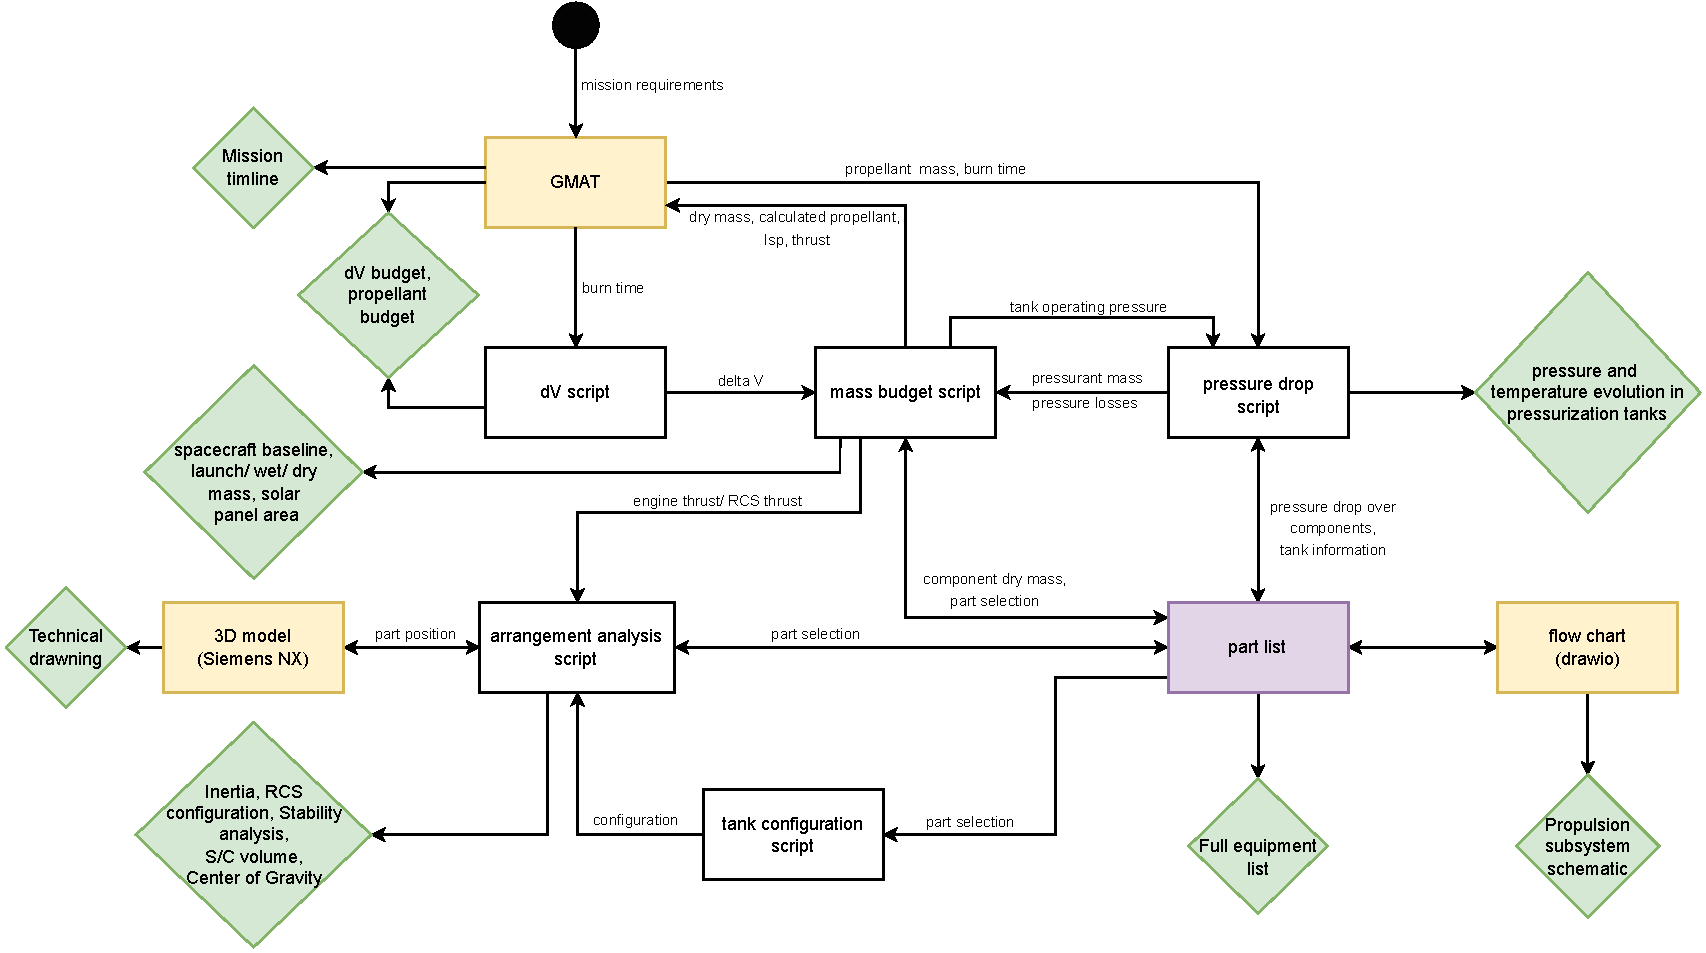
\includegraphics[width=0.8\textwidth]{img/work_flow.pdf}
  \caption{Flowchart of workflow}
  \label{fig:flow-work}
\end{figure*}

\subsection{GMAT}

The General Mission Analysis Tool (GMAT) is used to compute the trajectory and simulate the mission in space and time.
Hereby the mission was first implemented impulsive, then with finite chemical burns and ultimately with additional  finite electric burns in \href{https://github.com/Sven-J-Steinert/MomenTUM/blob/main/GMAT/MomenTUM_finite.script}{\colorbox{codegray}{MomenTUM\_finite.script}}.
As an output of this simulation, a result file \href{https://github.com/Sven-J-Steinert/MomenTUM/blob/main/GMAT/result/result.txt}{\colorbox{codegray}{result.txt}} is created, holding certain events by their timestamp and fuel level as well as burn-times and key-variables of the mission. This rather long file is shortened to the most important lines by a small script \href{https://github.com/Sven-J-Steinert/MomenTUM/blob/main/GMAT/cleaning.py}{\colorbox{codegray}{cleaning.py}} into \href{https://github.com/Sven-J-Steinert/MomenTUM/blob/main/GMAT/result/result_clean.txt}{\colorbox{codegray}{result\_clean.txt}}. Additionally the distance to Phobos is outputted by GMAT and plotted by 
\href{https://github.com/Sven-J-Steinert/MomenTUM/blob/main/GMAT/plot.py}{\colorbox{codegray}{plot.py}}.


\subsection{dv Script}

The delta v script \href{https://github.com/Sven-J-Steinert/MomenTUM/blob/main/MATLAB/dV_calc.m}{\colorbox{codegray}{dV\_calc.m}} is a program written in MATLAB. It's function is to take a given spacecraft dry mass, as well as the thrust and ISP of the engine used in the maneuvers, together with the dedicated burn-times from GMAT per maneuver. These values are then transformed into the respective delta v and propellant mass of each maneuver via the Tsiolkovsky rocket equation \cite{Walter.2018}.

\subsection{Mass Budget Script}
\label{script:mass-design}

To compute the launch mass of the spacecraft as well as the solar array size and the engine performance data, a mass budget script \href{https://github.com/Sven-J-Steinert/MomenTUM/blob/main/MATLAB/mass_design.m}{\colorbox{codegray}{mass\_design.py}}, written in MATLAB, is used. Here, the delta v's and the pressurant mass are needed as an input, while especially the spacecraft dry mass and engine performance is inserted back into GMAT as an output of this script. In this script, the ESA margin philosophy \cite{ESA.2012} is respected.

\subsection{Pressure Script}

The amount of pressurant required for the mission is calculated using the MATLAB pressure script \href{https://github.com/Sven-J-Steinert/MomenTUM/blob/main/MATLAB/pressure_temp_sim.m}{\colorbox{codegray}{pressure\_temp\_sim.m}}. The required inputs for the tool are the \href{https://github.com/Sven-J-Steinert/MomenTUM/blob/main/GMAT/result/result_clean.txt}{\colorbox{codegray}{result\_clean.txt}} file coming from GMAT transformed to a \href{https://github.com/Sven-J-Steinert/MomenTUM/blob/main/MATLAB/GMAT_values_20.xlsx}{\colorbox{codegray}{.xlsx}} file, as well as the pressurant and propellant tank characteristics (volumes and mean operating pressures). The outputs of this script are:
\begin{itemize}
    \item the total helium mass within the whole system at the beginning of operation, which is fed back to GMAT.
    \item the amount of helium within both pressurant and propellant tanks throughout the maneuvers.
    \item the pressure and temperature changes of helium within the pressurant and propellant tanks during the maneuvering time.
\end{itemize}


\subsection{Arrangement Analysis Script}

The spacecraft's configuration is determined by the arrangement analysis script \href{https://github.com/Sven-J-Steinert/MomenTUM/blob/main/MATLAB/arrangement_analysis.m}{\colorbox{codegray}{arrangement\_analysis.m}}, written in MATLAB. In this script, the orbital stability criteria for the spacecraft are matched with the spacecrafts geometrical layout and placement of the individual internal parts. This then results in a shape which directly influences the placement of the reaction control system (RCS). By the correct placement of the RCS thrusters, a combined main-engine placement offset and misalignment can be compensated, resulting in a resilient spacecraft design. A 3D model can then be derived from this configuration and fed back to indicate if the internal parts fit within the restricted volume. The spacecraft's volume, the shifting center of gravity (CoG) and the moments of inertia are an output of this analysis which can then be compared to the requirements of the launch vehicle \cite{Arianspace.2016}. 

\section{Mission Analysis and Overall Spacecraft}
\subsection{Mission Requirements}

The mission requirements form the baseline of the design process and are directly given in the design challenge \cite{Manfletti.2022}.

\begin{table}[H]
\centering
\caption{Mission Requirements \cite{Manfletti.2022}}
\label{tab:mis-req}
\begin{tblr}{
  row{1} = {Cornflower},
  row{2} = {Spindle},
  hlines,
  vline{1,3} = {1}{},
  vline{-} = {2-8}{},
}
                 & \textbf{Mission Requirements}                                                                                                                                                                     \\
\textbf{Req. ID} & \textbf{Statement}                                                                                                                                                                                \\
MIS.001          & {The system shall send a satellite to Phobos which will \\release a surface probe to Phobos ,one of the moons \\of Mars, to study its origin as well as its physical and \\chemical composition.} \\
MIS.002          & {The satellite shall be launched by a dedicated \\Ariane 62}                                                                                                                                      \\
MIS.003          & The total system mass shall not exceed 2600 kg.                                                                                                                                                   \\
MIS.004          & The launch date shall lay between 2026 and 2029.                                                                                                                                                  \\
MIS.005          & {The system shall reach an orbit around Phobos \\(Quasi-Satellite Orbit (QSO)) for a minimum of \\2 years to study Phobos from space and to serve \\as a relay for the surface probe.}            \\
MIS.006          & {At end of life (EOL) the spacecraft shall be \\de-orbited into the martian atmosphere (40km \\altitude at periapsis).}                                                                           
\end{tblr}
\end{table}

\subsection{Basic Mission Trajectory}
For a transit to Mars, multiple launch windows are possible within the required launch frame of 2026 to 2029 (MIS.004). The most interesting opportunities are the energy minima Type 2 transfers in 2026 \cite{Burke.2010} where the required characteristic energy (C3) and arrival excess speed are particularly low. In order to offer a safety margin in case of any delays, the second most optimal window, starting at 31.10.2026 was chosen which takes place before the most optimal one at 6.11.2026. So in a case of emergency the launch date can be prospered while still being able to fly the mission with the same hardware.

The trajectory starts by its carrier, an Ariane 62 (MIS.002) and its ejection on its outgoing asymptote. However, the mission launch opportunity requires 9.144 km²/s² of C3 where the Ariane 62 can only supply a infinity velocity of 2.5 km/s (6.25 km²/s² C3). Therefore the first maneuver is performed to match the required C3, when the spacecraft is leaving the influence of earth. Next, a trajectory correction maneuver (TCM) is performed to target the arrival at Mars precisely. When arriving at Mars, a Mars orbit insertion (MOI) is performed to reduce the spacecraft access velocity to a high elliptical orbital velocity. When crossing Phobos orbital plane, an inclination change is done near to the spacecrafts apoapsis followed by a raise of its periapsis to intersect with Phobos orbit. To match the point in time where Phobos and the spacecraft align, a parking orbit is created where after one round-trip, Phobos is matched with a deceleration burn where now its orbital parameters are similar to achieve a quasi satellite orbit. For the required delta v to perform orbital maintenance, literature values for this case have been used as $\frac{1.16}{8.23}$ m/s delta v per day \cite{Chen2020} and the mission duration MIS.005 plus margin. Ultimately as MIS.006 requires, the spacecraft is deorbited into the martian atmosphere through a deceleration burn at its apoapsis. The full set of delta v magnitudes for this impulsive trajectory and its V,N,B vector components are listed in table \ref{tab:man-dv-imp} corresponding to \href{https://github.com/Sven-J-Steinert/MomenTUM/blob/main/GMAT/MomenTUM_impulsive.script}{\colorbox{codegray}{MomenTUM\_impulsive.script}}.

\begin{table}[H]
\centering
\caption{Required DeltaV for Impulsive Maneuvers}
\label{tab:man-dv-imp}
\begin{tblr}{
  column{3} = {r},
  cell{1}{2} = {Cornflower,c},
  cell{1}{3} = {Cornflower,c},
  cell{1}{5} = {Cornflower,c},
  cell{1}{6} = {Cornflower},
  cell{1}{7} = {Cornflower},
  cell{2}{1} = {Cream},
  cell{2}{5} = {c},
  cell{2}{6} = {c},
  cell{2}{7} = {c},
  cell{3}{1} = {Cream},
  cell{3}{5} = {c},
  cell{3}{6} = {c},
  cell{3}{7} = {c},
  cell{4}{1} = {Cream},
  cell{4}{5} = {c},
  cell{4}{6} = {c},
  cell{4}{7} = {c},
  cell{5}{1} = {Cream},
  cell{5}{5} = {c},
  cell{5}{6} = {c},
  cell{5}{7} = {c},
  cell{6}{1} = {BabyBlue},
  cell{6}{5} = {c},
  cell{6}{6} = {c},
  cell{6}{7} = {c},
  cell{7}{1} = {BabyBlue},
  cell{7}{5} = {c},
  cell{7}{6} = {c},
  cell{7}{7} = {c},
  cell{8}{1} = {BabyBlue},
  cell{8}{5} = {c},
  cell{8}{6} = {c},
  cell{8}{7} = {c},
  cell{9}{1} = {BabyBlue},
  cell{9}{4} = {r},
  cell{9}{5} = {c},
  cell{9}{6} = {c},
  cell{9}{7} = {c},
  cell{10}{1} = {BabyBlue},
  cell{10}{5} = {c},
  cell{10}{6} = {c},
  cell{10}{7} = {c},
  cell{11}{2} = {Spindle},
  cell{11}{3} = {Spindle},
  vline{2-8} = {1}{},
  vline{-} = {2-10}{},
  vline{2-4} = {11}{},
  hline{1} = {2-3,5-7}{},
  hline{2-11} = {1-3,5-7}{},
  hline{12} = {2-3}{},
}
  & \textbf{Maneuver Name} & \textbf{ Magn. [m/s]} &  & \textbf{V} & \textbf{N} & \textbf{B} \\
C & Match C3               & 509.350               &  & x          &            &            \\
C & TCM                    & 34.553                &  & x          & x          & x          \\
C & MOI                    & 751.782               &  & x          &            &            \\
C & Match INC              & 13.153                &  &            & x          &            \\
E & Raise Peri             & 35.660                &  & x          &            &            \\
E & Parking Insertion      & 197.507               &  & x          &            &            \\
E & Match Phobos           & 640.000               &  & x          &            &            \\
E & Orbital Maintenance    & 104.950               &  & x          & x          & x          \\
E & EOL                    & 561.664               &  & x          &            &            \\
  & \textbf{Total}         & \textbf{2848.619}     &  &            &            &            
\end{tblr}
\end{table}

\subsection{Propulsion System Trade-off}
\label{subsection:PropSysTradeOff}

To analyze which propulsion system combination shall be used for this mission, the following trade-off, depicted in Table \ref{tab:prop-tradeoff} is conducted. The objective is to select the configuration with the minimum launch mass, which is calculated by the mass budget script. The mission delta v used in this comparison originates from a finite chemical implementation of the impulsive trajectory \href{https://github.com/Sven-J-Steinert/MomenTUM/blob/main/GMAT/MomenTUM_biprop_only.script}{\colorbox{codegray}{MomenTUM\_biprop\_only.script}}. The maneuvers Raise Peri to EOL are considered done electrically in a mixed system. In this analysis, if a maneuver is performed with an electric engine, the delta v is doubled because of the high uncertainty in regard to the continuous thrust maneuvers. In this simplified case, only the biprop-electric and the biprop propulsion system fulfil MIS.003 and stay below the 2600 kg capability of the launcher \cite{Arianspace.2016}. Since the biprop-electric system has the lowest launch mass and the doubling of the delta V for the electrical maneuvers is assumed conservatively high, the lightest propulsion system is expected to be the combination of a bipropellant and electric propulsion. A more detailed comparison between the bipropellant only and the biprop-electric system can be found in the Appendix \ref{Appendix}.

\begin{table}[H]
\caption{Propulsion System Trade-off}
\label{tab:prop-tradeoff}
\resizebox{\linewidth}{!}{%
\begin{tblr}{
  row{1} = {Cornflower,c},
  row{2} = {c},
  cell{1}{1} = {c=6}{},
  cell{3}{2} = {r},
  cell{3}{3} = {r},
  cell{3}{4} = {r},
  cell{3}{5} = {r},
  cell{3}{6} = {r},
  cell{4}{2} = {r},
  cell{4}{3} = {r},
  cell{4}{4} = {r},
  cell{4}{5} = {r},
  cell{4}{6} = {r},
  hlines,
  vlines,
}
\textbf{Propulsion System Trade-off} &                    &        &          &                      &          \\
Propulsion   System                  & {Biprop\\Electric} & Biprop & Electric & {Monoprop\\Electric} & Monoprop \\
Total Mission dV [m/s]               & 4698.2             & 3277.5 & 6555.0   & 4698.2               & 3277.5   \\
Launch Mass [kg]                     & 2124.4             & 2128.3 & 2878.3   & 3022.8               & 6949.7   
\end{tblr}}
\end{table}



\subsection{Advanced Mission Trajectory}
To apply the selected bipropellant and electric system, the trajectory has to be adapted. For the bipropellant section, the general approach of maneuvers can be kept, since their burn-times are comparably short. Besides the C3 maneuver, which has no time constrains, only the MOI critically spreads over a longer range of space and time as seen in Figure \ref{fig:chem-overview}.

\begin{figure}[H]
  \centering
  \includegraphics[width=\linewidth]{img/chem_overview.png}
  \caption{Chemical maneuvers: MOI, Match INC, Raise Peri min}
  \label{fig:chem-overview}
\end{figure}

After the inclination change and raising the periapsis to a minimum, the maneuvers are carried out by the electric propulsion in a different approach. The first electric section is the circularization of the orbit through a loop of burns by true anomaly which can be seen in figure \ref{fig:circularization} where yellow sections represent thrust arcs. The over-raise in periapsis comes for the benefit of drastically reduced flight-time and the over-raising is therefore a compromise of minimal delta v and flight-time.

\begin{figure}[H]
  \centering
  \includegraphics[width=\linewidth]{img/el_circularization.png}
  \caption{Electric maneuver: Circularization}
  \label{fig:circularization}
\end{figure}

From there on, the electric thruster continuously fires to spiral down and approach Phobos. The very low eccentricity of Phobos is capitalized on here, so that a matching can be achieved from a circular spiral. To match the intersection with Phobos correctly in time, the spiraling is paused (displayed green in Figure \ref{fig:spiral}) before its spiraling achieves a semi major axis of 9378.8 km and therefore a matching orbital period.

\begin{figure}[H]
  \centering
  \includegraphics[width=\linewidth]{img/el_sprial.png}
  \caption{Electric maneuver: Spiral Down Match}
  \label{fig:spiral}
\end{figure}

The Orbital Maintenance is assumed as in the impulsive section and its corresponding fuel mass is deducted. The EOL maneuver is also a loop of thrust arcs that decelerate the spacecrafts around its apoapsis, marked by true anomaly which can be seen in Figure \ref{fig:eol}. Hereby the assumption of 10 times the thrust equals to $\frac{1}{10}$ of the nominal burn-time was made to reduce computation time. This concludes the finite simulation of the selected bipropellant electrical system carried out in the GMAT script \href{https://github.com/Sven-J-Steinert/MomenTUM/blob/main/GMAT/MomenTUM_finite.script}{\colorbox{codegray}{MomenTUM\_finite.script}}.

\begin{figure}[H]
  \centering
  \includegraphics[width=\linewidth]{img/el_eol.png}
  \caption{Electric maneuver: EOL}
  \label{fig:eol}
\end{figure}

\subsection{deltaV Budget}

As a result of the now fully specified trajectory and its finite simulation, the maneuver delta vs and burn times are given precisely in Table \ref{tab:budget-dv} below.

\begin{table}[H]
\centering
\caption{DeltaV Budget}
\label{tab:budget-dv}
\resizebox{\linewidth}{!}{%
\begin{tblr}{
  row{1} = {Cornflower},
  row{2} = {Spindle},
  row{8} = {Spindle},
  row{13} = {Spindle},
  row{14} = {Cornflower},
  column{even} = {c},
  column{3} = {r},
  cell{1}{3} = {c},
  cell{2}{3} = {c},
  cell{3}{4} = {r},
  cell{4}{4} = {r},
  cell{5}{4} = {r},
  cell{6}{4} = {r},
  cell{7}{4} = {r},
  cell{8}{4} = {r},
  cell{9}{4} = {r},
  cell{10}{4} = {r},
  cell{11}{4} = {r},
  cell{12}{4} = {r},
  cell{13}{4} = {r},
  cell{14}{4} = {r},
  hlines,
  vlines,
}
                       &                    & {[}m/s]           & {[}s]               \\
\textbf{Maneuver Name} & \textbf{Type}      & \textbf{Delta v}  & \textbf{Duration}   \\
C3                     & finite             & 516.868           & 2155.85             \\
TCM                    & finite             & 1.395             & 5.35                \\
MOI                    & finite             & 850.981           & 2858.31             \\
Match INC              & finite             & 14.550            & 42.44               \\
Raise Peri min         & finite             & 4.515             & 13.13               \\
Total Chemical         &                    & 1388.308          & 5075.07             \\
Circularize            & finite             & 713.753           & 10164236.2          \\
Spiral Down Match      & finite             & 831.526           & 11334710.2          \\
Orbital Maintenance    & stochastic         & 104.950           &                     \\
EOL                    & finite, assumption & 708.395           & 9035872.4           \\
Total Electric         &                    & 2358.624          & 30534818.8          \\
\textbf{Total}         &                    & \textbf{3746.932} & \textbf{30539893.9} 
\end{tblr}
}
\end{table}

An more in depth overview of the mission is put together in the mission timeline in Table \ref{tab:mis-timeline} that marks all states by a timestamp and their associated spacecraft values.


\subsection{Mass Budget}
The mass budget of the final spacecraft is depicted in Table \ref{tab:mas-bud}. It is generated by the mass budget script and lists all subsystems and propellants with their respective masses and margins. These margins are based on the ESA margin philosophy \cite{ESA.2012}. While most subsystem masses are already fixed for the mission, the STR and PWR subsystem need to be calculated via to following equations \cite{Manfletti.2022}. Regarding the STR subsystem, Equation \ref{eq:STR} is used, while for the PWR subsystem, Equation \ref{eq:PWR} shall be applied. In case of the CPROP and EPROP subsystem, commercial parts are chosen to form the subsystems total mass. For the launch adapter, the PLA6 1194 is used which can be found in the user's manual of the Ariane 62 \cite{Arianspace.2016}. In this budget, the dry mass is stated with the integrated Phobos surface probe, which is dropped in a later mission phase. This is because the harness and structural mass has to be sized for the probe as well, which then needs to be included. As a result, the dry mass is not a constant value over the whole mission.

\begin{equation}
m_{STR} = 0.0224 \cdot m_{wet} + 27.823
\label{eq:STR}
\end{equation}

\begin{equation}
m_{PWR} = 0.0758 \cdot P_{Earth} + 37.741
\label{eq:PWR}
\end{equation}

\begin{table}[H]
\centering
\caption{Mass Budget}
\label{tab:mas-bud}
\resizebox{\linewidth}{!}{%
\begin{tabular}{|lrr|}
\hline
\rowcolor[HTML]{8DB4E1} 
\multicolumn{3}{|l|}{\cellcolor[HTML]{8DB4E1}\textbf{SC Mass Budget}}                                         \\ \hline
\textbf{System}                                  & \textbf{Margin}                   & \textbf{Mass {[}kg{]}} \\ \hline
AOGNC                                            &                                   & 40.0                   \\ \hline
COM                                              &                                   & 25.0                   \\ \hline
CDH                                              &                                   & 15.0                   \\ \hline
CPROP                                            &                                   & 126.9                  \\ \hline
EPROP                                            &                                   & 45.4                   \\ \hline
INS                                              &                                   & 50.0                   \\ \hline
MEC                                              &                                   & 55.0                   \\ \hline
PWR                                              &                                   & 398.6                  \\ \hline
STR                                              &                                   & 73.9                   \\ \hline
TC                                               &                                   & 15.0                   \\ \hline
Probe                                            &                                   & 20.0                   \\ \hline
Harness                                          & 10\%                              & 86.6                   \\ \hline
\rowcolor[HTML]{C5D9F0} 
\textbf{Dry Mass}                                & \textbf{}                         & \textbf{951.3}         \\ \hline
System Margin                                    & 20\%                              &                        \\ \hline
\rowcolor[HTML]{C5D9F0} 
\multicolumn{2}{|l}{\cellcolor[HTML]{C5D9F0}\textbf{Dry Mass incl.   System Margin}} & \textbf{1141.6}        \\ \hline
CPROP Fuel   Mass                                &                                   & 736.0                  \\ \hline
CPROP Fuel   Margin                              & 2\%                               & 15.0                   \\ \hline
CPROP   Pressurant Mass                          &                                   & 3.5                    \\ \hline
CPROP   Pressurant Mass Margin                   & 2\%                               & 0.1                    \\ \hline
EPROP Fuel   Mass                                &                                   & 162.7                  \\ \hline
EPROP Fuel   Mass Margin                         & 2\%                               & 3.3                    \\ \hline
\rowcolor[HTML]{C5D9F0} 
\textbf{Total Wet   Mass}                        & \textbf{}                         & \textbf{2062.4}        \\ \hline
Launch   Adapter                                 &                                   & 85.0                   \\ \hline
\rowcolor[HTML]{C5D9F0} 
\textbf{Total Launch   Mass}                     & \textbf{}                         & \textbf{2147.4}        \\ \hline
\end{tabular}}
\end{table}

\subsection{Spacecraft Baseline}

As a result of the mass budget, the spacecraft baseline design can be derived, which is shown in Table \ref{tab:sc-bas}. In it, the chosen main components of the individual subsystems are displayed together with some key data. While the mass and the propulsion components, together with the heating system, are a direct optimized result of the iteration process between GMAT, the delta v budget, mass budget and pressure drop script, some other components are chosen on the basis of the Ice Giants mission from ESA \cite{ESA.2019}. The Phobos surface probe as a payload can be traced back to MIS.001 in Table \ref{tab:mis-req}. Especially the space frame design is chosen to keep the placement of the propulsion system components flexible.

\begin{table}[H]
\centering
\caption{Spacecraft Baseline}
\label{tab:sc-bas}
\resizebox{\linewidth}{!}{%
\begin{tblr}{
  row{1} = {Cornflower,c},
  cell{1}{1} = {c=2}{},
  hlines,
  vlines,
}
\textbf{Spacecraft Baseline Design} &                                                                                                                                                                                                                         \\
{Mass \\(incl. 20\% sys. margin)}   & {Dry mass: 1141.6 kg \\ Chemical propellant mass (excl. margin): 751.3 kg\\ Electrical propellant mass (excl. margin): 166.0 kg\\ Wet mass: 2062.4 kg}                                                                  \\
Payload                             & {Phobos surface probe\\ Phobos imager}                                                                                                                                                                                  \\
Propulsion                          & {1x main bipropellant thruster (450 N)\\ 12x RCS thruster (12 N)\\ 2x pressurant tank (40 l)\\ 1x bipropellant tank (331 l)\\ 2x bipropellant tank (198 l)\\ 1x electric thruster (0.090 N)\\ 2x noble gas tank (60 l)} \\
AOGNC                               & {1x coarse rate sensor\\ 2x navigation cameras\\ 2x IMUs\\ 2x star trackers\\ 4x reaction wheels\\ (+ RCS thrusters)}                                                                                                   \\
Communications                      & {X-band uplink/downlink\\ Ka-band downlink}                                                                                                                                                                             \\
Power                               & {2x solar array (2m x 7.5m)\\ Power Processing Unit (PPU) + internal batteries}                                                                                                                                         \\
Data Handling                       & {Redundant On-Board Computing (OBC)\\capability + storage}                                                                                                                                                              \\
Structures                          & Space frame design                                                                                                                                                                                                      \\
Thermal                             & {MLI insulation blankets\\ Heating system within the pressurant tanks}                                                                                                                                                  
\end{tblr}
}
\end{table}

%\vspace*{\fill}

\section{Chemical Propulsion System}
    
    
\subsection{Chemical Propulsion System Requirements}
The chemical propulsion system requirements in Table \ref{tab:sys-req} are derived from the mission requirements in Table \ref{tab:mis-req}.

\begin{table}[H]
\centering
\caption{Propulsion System Requirements}
\label{tab:sys-req}
\scalebox{0.9}{
\begin{tblr}{
  row{1} = {Cornflower},
  row{2} = {Spindle},
  hlines,
  vline{-} = {1-10}{},
}
                 & \textbf{Propulsion System Requirements}                                                                                                                                                                                                                   \\
\textbf{Req. ID} & \textbf{Statement}                                                                                                                                                                                                                                        \\
CPROP.001         & {The propulsion system shall provide the necessary \\thrust and delta v, required to perform \\the foreseen mission manoeuvers.}                                                                                                                      \\
CPROP.002         & {The propulsion system shall provide torques to \\compensate the main engine misalignments and \\for all other attitude and orbit control maneuvers, \\including safe-mode operation and reaction wheel \\off loading, as required by mission planning.} \\
CPROP.003         & {The subsystem shall have inhibits against critical \\failures leading to personnel hazard (e.g. while \\handling the spacecraft)}                                                                                                                        \\
CPROP.004         & {The propulsion system shall include single failure \\tolerant measurement of the propellant pressure.}                                                                                                                                              \\
CPROP.005         & {The propulsion system shall provide means to \\isolate potential external leakages and/or failures \\of thruster flow control valves.~~}                                                                                                                 \\
CPROP.006         & {The propulsion system shall include access \\points (valves) for filling and draining the \\propulsion system on ground.}                                                                                                                          \\
CPROP.007         & {All components within the propulsion system \\shall be TRL9.}     
                                                            \\
CPROP.008         & {As many components as possible  within the \\ chemical propulsion system shall be of european\\ origin.}  

\end{tblr}
}
\end{table}

\subsection{Assumptions}
For the chemical propulsion system design the assumptions listed in Table \ref{tab:prop-assumptions} were used for the calculations.
\begin{table}[H]
\centering
\caption{Assumptions}
\label{tab:prop-assumptions}
\resizebox{\linewidth}{!}{%
\begin{tblr}{
  row{1} = {Cornflower},
  vline{1,3} = {1,3}{},
  vline{1,3} = {2-4}{},
  hline{1,3-5} = {-}{},
}
  & \textbf{Assumptions}                                                                                                                                                                                                             \\
1 & {The overall ISP for
the
bipropellant engine is
assumed to
\\be
an average between the
main engine
and RCS thrusters \\weighed by
their
thrust
} \\
2 & {The power required at Mars was scaled with
respect to
\\the
power requirement in Earth using
the
inverse \\square law.}                       
\end{tblr}
}
\end{table}

\subsection{Chemical System Trade-offs}
\label{subsection:ChemSysTradeOff}

The initial system trade-offs in Section \ref{subsection:PropSysTradeOff} resulted in the selection of a bipropellant chemical subsystem over monopropellant. The application of this subsystem as part of an upper stage engine with low thrust range ($<$ 40 kN) leads to the selection of a pressure fed cycle \cite{Manfletti.2022}.
A dual-mode bipropellant system was disregarded since the bipropellant engine is relevant during the initial high-thrust phase of the mission, and the flexibility of switching to low-thrust, high-specific impulse propulsion is already provided by the electric propulsion subsystem.

Two main trade-off's were conducted for the bipropellant chemical subsystem design: the thruster selection process and the tank configuration. 

The thruster selection was driven by requirements derived from the mission analysis calculations, which define a required thrust higher than 400 N, and a longest burn time of around 3000 s. The following thrusters were considered: Ariane S400-12, Ariane S400-15, NAMMO LEROS 2b and Aerojet Rocketdyne R-4D-15 HiPAT™. All these options fit the mission analysis requirements regarding thrust range, ISP, and oxidizer to fuel ratio. The Aerojet thruster was dismissed due to its US origin (CPROP.008). With the remaining European thrusters, the driver of the trade-off was the launch mass, which resulted the lower for the selected thruster: Ariane S400-15, as shown in Table \ref{tab:thruster-tradeoff} \cite{Ariane.2023}. 
\begin{table} [H]
\centering
\caption{Bipropellant Main Thruster Trade-off}
\label{tab:thruster-tradeoff}
\resizebox{\linewidth}{!}{%
\begin{tabular}{|l|r|l|r|r|} 
\hline
\rowcolor[rgb]{0.553,0.706,0.882} \multicolumn{1}{|c|}{\textbf{Thruster}}            & \multicolumn{1}{c|}{\textbf{Launch mass [kg]}}        & \multicolumn{1}{c|}{Thrust [N ]}                     & \multicolumn{1}{c|}{Burn Time [s]~}      & \multicolumn{1}{c|}{ISP [s]}                 \\ 
\hline
Ariane~\textcolor[rgb]{0.122,0.122,0.122}{S400-12}                                   & \textcolor[rgb]{0.122,0.122,0.122}{1584.494}          & \textcolor[rgb]{0.122,0.122,0.122}{340 to 440 [420]} & \textcolor[rgb]{0.122,0.122,0.122}{3960} & \textcolor[rgb]{0.122,0.122,0.122}{318.000}  \\ 
\hline
\rowcolor[rgb]{0.992,0.863,0.506} \textcolor[rgb]{0.122,0.122,0.122}{Ariane S400-15} & \textcolor[rgb]{0.122,0.122,0.122}{\textbf{1578.371}} & \textcolor[rgb]{0.122,0.122,0.122}{342 to 440 [425]} & 6600                                     & \textcolor[rgb]{0.122,0.122,0.122}{321.000}  \\ 
\hline
\textcolor[rgb]{0.122,0.122,0.122}{NAMMO LEROS 2b}                                   & \textcolor[rgb]{0.122,0.122,0.122}{1584.663}          & \textcolor[rgb]{0.122,0.122,0.122}{367 to 456 [420]} & 6600                                     & \textcolor[rgb]{0.122,0.122,0.122}{319.500}  \\ 
\hline
\multicolumn{1}{l}{Nominal values in []}                                             & \multicolumn{1}{r}{}                                  & \multicolumn{1}{l}{}                                 & \multicolumn{1}{r}{}                     & \multicolumn{1}{r}{}                        
\end{tabular}
}
\end{table}
The selected propellant combination is Monomethylhydrazine (MMH) and mixed oxides of nitrogen (MON-3). The fuel is defined by the thruster specification. With respect to the oxidizer, the thruster enabled using Nitrogen Tetroxide (NTO), MON-1 or MON-3. MON was selected over NTO due to its lower sensitivity to temperature fluctuations and the higher availability of European tanks with demonstrated compatibility. MON-3 was chosen over MON-1 because it has a lower vapor pressure, making it easier to handle and safely store before and during the mission. %include source

A further trade-off determined number of propellant tanks required. Figure \ref{fig:biprop-tank-config} shows the options considered, whereby the propellant tanks are from Ariane Group and the pressurant tanks from MT Aerospace (CPROP.007 and CPROP.008).
\begin{figure} [H]
    \centering
    \includegraphics[width=\linewidth]{img/BipropConfig.png}
    \caption{Bipropellant Tanks Configuration Trade-off}
    \label{fig:biprop-tank-config}
\end{figure}
The lightest option is configuration 4, however later stability analysis explained in Section \ref{subsection:sc-stab-anal} proved it unsuitable. Therefore, the next lightest and thus selected configuration includes one 331 l MMH tank, two 198 l MON tanks and 2 40 l helium tanks. 

The rest of the subsystem is developed around the selected thruster and tank configuration. It will be described in detail in the following sections.


\subsection{Chemical Propulsion System Architecture}

In this chapter the architecture overview of the whole bipropellant subsystem will be given and technical decisions derived from the system requirements will be justified.
The Chemical propulsion subsystem was developed to fulfill specific system requirements, stated in Table \ref{tab:sys-req}, and assumptions depicted in the Table \ref{tab:mis-assumptions} and it is unique technical solution. The flow chart of the chemical subsystem with all the relevant details is shown in Figure \ref{fig:flow-biprop} in the Appendix \ref{Appendix}. From the mission design it is derived that the first five maneuvers are performed using chemical propulsion including MOI which is the most demanding one concerning the overall propulsion subsystem. The main engine S400-15 from ArianeGroup shall provide the necessary thrust for this orbit insertion maneuver, the trajectory correction maneuver and remaining maneuvers while twelve ArianeGroup RCS thrusters S10-26 shall provide the thrust for a 3-axis attitude control once arrived in orbit around Phobos for at least two years. These two off the shelf bipropellant thrusters meet the requirements of this mission and are chosen also considering economic reasons and heritage of around 40 completed missions for the S400-12 and S400-15 engines. Both selected thrusters are helium pressurized and use monomethyl-hydrazine (MMH) as fuel and  mixed oxides of nitrogen MON-3 as oxidizer. From the flow chart it is visible that two 40 liter tanks are used for pressurized helium. To fill the tanks and access the fluid, fill and drain valves are placed after every tank. Helium is leaving the pressurant tanks with 310 bar and goes through a dual mechanical pressure regulator which lowers the pressure to 20 bar. Normally closed pyro valves are placed before and after pressure was regulated to isolate it in case of any leakage. Redundant check valves are ensuring that the flow is going only in the direction of the propellant tanks and safety relief valves are placed in case of any kind of over pressurisation of helium before entering the pressurization tanks. To secure that propellants are not going upstream and mixing with helium, normally closed pyro valves are placed before the propellant tanks. In the feed line of the main engine, pyro ladders are introduced and are chosen due to their redundancy and minimum leakage. Furthermore, the mission is designed in a way that the main engine is passivated in between the second and third maneuver due to long waiting time as well as after fifth (last chemical) maneuver which leads to a possible leakage of propellants. The pyro ladder will isolate main engine during these periods and ensures redundant access to the main engine. Upstream the RCS thrusters latch valve is placed to control the propellant flow for attitude control. The latch valves are used because of their ability to open and close numerous times which is advantageous in the case of attitude control. The S10-26 are dual seat thursters meaning they have two flow control valves serially connected which allow a more precise attitude control and the shutdown of a thruster in case of a failure or malfunction.


\subsection{Chemical Propulsion System Mass Budget}

To compute the dry mass of the chemical subsystem, the component selection is iterated throughout the development process to ensure a failure free mission by choosing off the shelf equipment while taking into account heritage from already completed missions. The current baseline consists of the equipment listed in the Table \ref{tab:equ-lis}. One of the assumptions of this mission is to have an all European component design, but at this point of development some of the selected components are outside of Europe and are marked in orange. In future development steps, this should be replaced with European components to fulfill the CPROP.008 requirement and reduce cost. Taking into account the ESA margin philosophy \cite{ESA.2012}, a margin of 20\% is applied on pipes and 5\% for off the shelf components.

\vspace*{\fill}

\begin{table}
\centering
\caption{Bipropellant Part List}
\label{tab:equ-lis}
\resizebox{\linewidth}{!}{%
\begin{tabular}{|l|l|r|r|r|r|} 
\hline
\rowcolor[rgb]{0.553,0.706,0.882} Description                & Type/Manufacturer                                 & Amount               & \begin{tabular}[c]{@{}>{\cellcolor[rgb]{0.553,0.706,0.882}}r@{}}Mass per~\\unit [kg]\end{tabular} & Margin               & \begin{tabular}[c]{@{}>{\cellcolor[rgb]{0.553,0.706,0.882}}r@{}}Mass inc.\\margin\end{tabular}  \\ 
\hline
Pipes                                                        & Pipes                                             & 1                    & 2.540                                                                                             & 0.2                  & 3.048                                                                                           \\ 
\hline
Main Engine                                                  & S400-15                                           & 1                    & 5.200                                                                                             & 0.05                 & 5.460                                                                                           \\ 
\hline
RCS Thruster                                                 & S10-26                                            & 12                   & 1.800                                                                                             & 0.05                 & 8.190                                                                                           \\ 
\hline
Helium Tank                                                  & PVG Family 40l                                    & 2                    & 8.500                                                                                             & 0.05                 & 18.700                                                                                          \\ 
\hline
Fuel Tank                                                    & OST 25/0                                          & 1                    & 21.000                                                                                            & 0.05                 & 22.050                                                                                          \\ 
\hline
Oxide Tank                                                   & OST 25/0                                          & 2                    & 21.000                                                                                            & 0.05                 & 44.100                                                                                          \\ 
\hline
Fill  Vent Valve                                             & ArianeGroup                                       & 3                    & 0.060                                                                                             & 0.05                 & 0.315                                                                                           \\ 
\hline
Latch Valve                                                  & ArianeGroup                                       & 4                    & 0.545                                                                                             & 0.05                 & 2.289                                                                                           \\ 
\hline
Pyro Isolation Valve                                         & ArianeGroup                                       & 16                   & 0.160                                                                                             & 0.05                 & 2.688                                                                                           \\ 
\hline
Safety Relief Valve                                          & Safran                                            & 2                    & 0.700                                                                                             & 0.05                 & 1.470                                                                                           \\ 
\hline
Check Valve                                                  & {\cellcolor[rgb]{1,0.831,0.541}}Vacco             & 4                    & 0.020                                                                                             & 0.05                 & 0.084                                                                                           \\ 
\hline
Filter                                                       & {\cellcolor[rgb]{1,0.831,0.541}}Vacco             & 8                    & 1.500                                                                                             & 0.05                 & 12.600                                                                                          \\ 
\hline
Dual Pressure Regulator                                      & {\cellcolor[rgb]{1,0.831,0.541}}Stanford Mu       & 1                    & 1.130                                                                                             & 0.05                 & 1.187                                                                                           \\ 
\hline
Pressure Transducer                                          & {\cellcolor[rgb]{1,0.831,0.541}}Bradford Space    & 5                    & 0.230                                                                                             & 0.05                 & 1.207                                                                                           \\ 
\hline
Thermocouples                                                & {\cellcolor[rgb]{1,0.831,0.541}}Collins Aerospace & 12                   & 0.350                                                                                             & 0.05                 & 4.410                                                                                           \\ 
\hline
\rowcolor[rgb]{0.773,0.851,0.941} \multicolumn{1}{|l}{Total} & \multicolumn{1}{l}{}                              & \multicolumn{1}{r}{} & \multicolumn{1}{r}{}                                                                              &                      & 126.948                                                                                         \\ 
\hline
\multicolumn{1}{l}{}                                         & \multicolumn{1}{l}{}                              & \multicolumn{1}{r}{} & \multicolumn{1}{r}{}                                                                              & \multicolumn{1}{r}{} & \multicolumn{1}{r}{}                                                                            \\
\multicolumn{1}{l}{}                                         & \multicolumn{1}{l}{}                              & \multicolumn{1}{r}{} & \multicolumn{1}{r}{}                                                                              & \multicolumn{1}{r}{} & \multicolumn{1}{r}{}                                                                           
\end{tabular}
}
\end{table}

\subsection{Chemical Propellant Budget}

\begin{table}[H]
\centering
\caption{Chemical Propellant Budget}
\label{tab:budget-prop-chem}
\resizebox{0.65\linewidth}{!}{%
\begin{tblr}{
  row{1} = {Cornflower},
  row{2} = {Spindle},
  row{8} = {Spindle},
  row{12} = {Spindle},
  row{13} = {Cornflower},
  column{2} = {r},
  column{3} = {r},
  cell{1}{2} = {c},
  cell{1}{3} = {c},
  cell{2}{2} = {c},
  cell{2}{3} = {c},
  hlines,
  vlines,
}
                       & {[}kg]           & {[}kg]           \\
\textbf{Maneuver Name} & \textbf{MMH}     & \textbf{MMO}     \\
C3                     & 116.714          & 192.578          \\
TCM                    & 0.290            & 0.478            \\
MOI                    & 155.285          & 256.221          \\
Match INC              & 2.298            & 3.791            \\
Raise Peri min         & 0.169            & 0.280            \\
Total Chemical         & 274.756          & 453.348          \\
Margin 1\% AOGNC       & 2.748            & 4.533            \\
Margin 2\%             & 5.495            & 9.067            \\
Margin Sum             & 8.243            & 13.600           \\
Leftover               & 8.744            & 14.427           \\
\textbf{Total}         & \textbf{283.500} & \textbf{467.775} 
\end{tblr}
}
\end{table}

\subsection{Helium Fill Level, Pressure and Temperature in Pressurant and Propellant Tanks}
\label{subsection:PressCalc}

The feeding system for the propellant tanks is pressure regulated to enable for consistent and predictable performance and to optimize fuel efficiency, which is important for a long-duration mission. A pressure regulated system requires the pressurant gas to be stored in additional tanks. In the presented bipropellant system, the propellant tanks are pressurized with Helium stored in two 40-liter tanks from MT Aerospace \cite{MTTankka92:online}. 

The options considered as a pressurant gas were helium and nitrogen, which were determined by the selected propellant tanks. Helium is used as a pressurant gas due to the following advantages over nitrogen: 
\begin{itemize}
    \item its lower density, which means it can provide the same pressure at lower mass or volume 
    \item a lower viscosity, useful for precise flow control and better flow over small orifices and valves
    \item it is non-reactive even at high temperatures and pressures, making it ideal for use in a pressurized system where contamination or chemical reactions can be a concern
\end{itemize}
However, there are also some disadvantages to using helium over nitrogen. For example, helium is more expensive and less widely available than nitrogen, which can make it less cost-effective. Nonetheless, its low density and thus reduction of the launch mass is the deciding factor in favour of helium.

To guarantee the required operation of the bipropellant chemical thrusters, thereby contributing to requirement CPROP.001, a thorough analysis of the Helium fluidic conditions throughout the bipropellant engine operation is performed. This analysis is based on the assumptions listed on Table \ref{tab:press-assumptions}.
\begin{table} [H]
\centering
\caption{Assumptions Pressurant Tank Sizing}
\label{tab:press-assumptions}
\resizebox{\linewidth}{!}{%
\begin{tblr}{
  row{1} = {Cornflower},
  vline{1,3} = {-}{},
  hline{1,3-7} = {-}{},
}
  & \textbf{Assumptions}                                                                                                                                                                                    \\
1 & {The initial ullage volume in the propellant tanks is filled with Helium before the \\start of operation.}                                                                                              \\
2 & {The temperature of Helium in the propellant tanks is calculated as the equilibrium \\temperature between the Helium in the tank and the incoming Helium from the \\pressure regulator.}                \\
3 & {The temperature increase of Helium over the pressure regulator due to the \\Joule-Thomson effect is averaged over the maneuvre time with the conditions \\at the beginning and end of the maneuvre.} \\
4 & {Heat transfer in Helium within the propellant tanks at the liquid-vapour interface \\and at the tank walls is neglected.}  \\ 
5 & {The required combustion chamber inlet pressure is 18.5 bars and the pressure drop \\between the propellant tanks and the thruster is 1.5 bars,\\leading to a required propellant tank pressure of 20 bars} 
\end{tblr}
}
\end{table}
For the propulsion system design, one of the most relevant parameters is the amount of helium required in the system since it influences the launch mass, both directly as additional wet mass and indirectly as it affects dry mass of the required pressurant tanks. In order to maintain the required engine operation, the pressurization system shall contain enough helium for all foreseen maneuvers and at least an additional ullage mass of 20 \%. Table \ref{tab:press-tank-mar} shows the fulfillment of these conditions. 
\begin{table}[H]
\centering
\caption{Pressurant Tank Margin}
\label{tab:press-tank-mar}
\resizebox{0.8\linewidth}{!}{%
\begin{tblr}{
  row{4} = {Spindle},
  row{5} = {Spindle},
  cell{1}{2} = {r},
  cell{2}{2} = {r},
  cell{3}{2} = {r},
  cell{4}{1} = {Spindle},
  cell{4}{2} = {r},
  hlines,
  vlines,
}
Initial Helium Mass in Pressurant Tank [kg] & 3.266  \\
Total Helium Mass maneuvers [kg]            & 1.961  \\
Leftover Helium in pressurant tank [kg]     & 1.305  \\
\textbf{Pressurant Mass Margin [\%]}       & 40.000 \\
Required Pressurant Mass Margin [\%]        & $\g$20.000 
\end{tblr}
}
\end{table}

Regarding the selection of the pressurant tanks, two suppliers were considered: Northrop Grumman and MT Aerospace. Despite the higher range of volumes offered by the Northrop Grumman \cite{Pressura17:online}, it was not selected because of its US origin (CPROP.008). The high-pressure helium tanks offered by MT aerospace have a Mean Operating Pressure (MEOP) of 310 bars, which results in a total volume of helium of 48 liters required for maneuvers. Considering an ullage volume of 20 \%, the volume of helium shall be at 57.6 $(m^3)$ \cite{Manfletti.2022}. Nevertheless, the sizing of the helium tanks is not only dependent on the required volume, but also on the helium pressure and temperature conditions, both in the propellant and in the helium tanks. 
For this reason, a fluidic simulation was performed with the following objectives:
\begin{itemize}
    \item guaranteeing safe propellant conditions;
    \item maintaining the pressure of helium within the pressurant tanks above the 20 bars required in the propellant tanks; 
    \item keeping the helium temperature within the pressurant tank between - 30 and + 60ºC as specified by the tank supplier (Table \ref{tab:pre-tan});
\end{itemize}
The calculated pressure and temperature conditions of helium within the pressurant tanks throughout the maneuvering time are depicted in figures \ref{fig:HeTempHeTank} and \ref{fig:HePressureHeTank}. For this calculation, only the first five maneuvers are considered, since the remaining maneuvers are not performed with the chemical engine. 
As observed in figure \ref{fig:HePressureHeTank}, the helium pressure is still above 100 bars after the last chemical maneuver, leaving more than enough margin for the RCS thruster operation. The temperature of helium within the pressurant tank remains between - 20 and + 50ºC, as depicted in figure \ref{fig:HePressureHeTank} fulfilling the aforementioned tank temperature constraint. In order to keep the temperature in this range, a heater is added to the pressurant tank. This heater is active in between maneuvers, as well as during the biggest maneuvers, which coincide with the biggest pressure and temperature drops in the charts: the first and third maneuver, namely C3 and MOI respectively.
\begin{figure}[H]
  \centering
  \includegraphics[width=0.8\linewidth]{img/HelliumPressureHeTank.png}
  \caption{Helium Pressure in Pressurant Tanks}
  \label{fig:HePressureHeTank}
\end{figure}
\begin{figure}[H]
  \centering
  \includegraphics[width=0.8\linewidth]{img/HeliumTempHeTank.png}
  \caption{Helium Temperature in Pressurant Tanks}
  \label{fig:HeTempHeTank}
\end{figure}
Table \ref{tab:press-tank-siz} displays the exact pressure and temperature values at the beginning and end of each chemical maneuver, as well as the heating power required. The pressurant tank is warmed up to 50 ºC before the beginning of operation and between the second and third maneuvers; and to 20 ºC before the last two chemical maneuvers. The maximum heater power required is 200 W during the MOI maneuver, which can be easily provided by the power system since at this point of operation, the electric engine is still not in use.
\begin{table}[H]
\centering
\caption{Pressurant Tank Sizing}
\label{tab:press-tank-siz}
\resizebox{\linewidth}{!}{%
\begin{tblr}{
  row{1} = {Cornflower},
  row{2} = {Spindle},
  row{4} = {r},
  row{6} = {r},
  row{9} = {r},
  row{12} = {r},
  row{14} = {r},
  row{15} = {Spindle},
  row{18} = {Spindle},
  column{2} = {r},
  column{3} = {r},
  cell{1}{2} = {c},
  cell{1}{3} = {c},
  cell{1}{4} = {c},
  cell{1}{5} = {c},
  cell{1}{6} = {Cornflower,c},
  cell{2}{2} = {c},
  cell{2}{3} = {c},
  cell{2}{4} = {c},
  cell{2}{5} = {c},
  cell{2}{6} = {Spindle,c},
  cell{3}{1} = {r=2}{},
  cell{3}{2} = {r=2}{},
  cell{3}{3} = {r=2}{},
  cell{3}{4} = {r},
  cell{3}{5} = {r},
  cell{3}{6} = {r=2}{r},
  cell{5}{1} = {r=2}{},
  cell{5}{2} = {r=2}{},
  cell{5}{3} = {r=2}{},
  cell{5}{4} = {r},
  cell{5}{5} = {r},
  cell{5}{6} = {r=2}{r},
  cell{7}{1} = {c=3}{},
  cell{7}{4} = {r},
  cell{7}{5} = {r},
  cell{7}{6} = {r},
  cell{8}{1} = {r=2}{},
  cell{8}{2} = {r=2}{},
  cell{8}{3} = {r=2}{},
  cell{8}{4} = {r},
  cell{8}{5} = {r},
  cell{8}{6} = {r=2}{r},
  cell{10}{1} = {c=3}{},
  cell{10}{4} = {r},
  cell{10}{5} = {r},
  cell{10}{6} = {r},
  cell{11}{1} = {r=2}{},
  cell{11}{2} = {r=2}{},
  cell{11}{3} = {r=2}{},
  cell{11}{4} = {r},
  cell{11}{5} = {r},
  cell{11}{6} = {r=2}{r},
  cell{13}{1} = {r=2}{},
  cell{13}{2} = {r=2}{},
  cell{13}{3} = {r=2}{},
  cell{13}{4} = {r},
  cell{13}{5} = {r},
  cell{13}{6} = {r=2}{r},
  cell{15}{1} = {c=2}{Spindle},
  cell{15}{3} = {Spindle},
  cell{16}{1} = {c=2}{},
  cell{17}{1} = {c=2}{},
  cell{18}{1} = {c=2}{Spindle},
  cell{18}{3} = {Spindle},
  vline{-} = {1-14}{},
  vline{5-6} = {4,6,9,12,14}{},
  vline{1-2,5-7} = {7,10}{},
  vline{1-2,7} = {15-18}{},
  hline{1-3,5,7-8,10-11,13,15-19} = {-}{},
}
                                        & {[}m/s]          & {[}kg]                   & {[}bar]           & {[}ºC]               & {[}W]           \\
\textbf{Maneuver Name}                 & \textbf{Delta v} & \textbf{Helium required} & \textbf{Pressure} & \textbf{Temperature} & \textbf{Heater} \\
C3                                      & 509.350          & 0.836                   & 310.000           & 50.000               & 50              \\
                                        &                  &                          & 177.175           & -17.479              &                 \\
TCM                                     & 34.553            & 0.002                    & 177.175           & -17.479             & OFF             \\
                                        &                  &                          & 176.903           & -17.635              &                 \\
Waiting time                            &                  &                          & 223.156           & 50.000               & $\leq$50              \\
MOI                                     & 751.782          & 1.105                    & 223.156           & 50.000               & 200             \\
                                        &                  &                          & 96.268            & -6.683              &                 \\
Waiting time                            &                  &                          & 105.854            & 20.000               & $\leq$50              \\
Match INC                               & 13.153           & 0.017                    & 105.854            & 20.000               & OFF             \\
                                        &                  &                          & 103.498            & 17.369               &                 \\
Raise Peri min                          & 35.660            & 0.001                    & 103.498            & 17.369               & OFF             \\
                                        &                  &                          & 103.332            & 17.184               &                 \\
Total Helium Mass maneuvers [kg]       &                  & 1.961                    &                   &                      &                 \\
Ullage Helium in propellant tanks [kg]  &                  & 0.259                    &                   &                      &                 \\
Leftover Helium in pressurant tank [kg] &                  & 1.305                    &                   &                      &                 \\
\textbf{Total Helium Mass [kg] }        &                  & 3.525                    &                   &                      &                 
\end{tblr}
}
\end{table}
As shown in the last four rows of the table, the total amount of helium required in the system is 3.525 kg, accounting for the helium within the pressurant tanks and the initial helium within the propellant tanks filling their ullage volume. The mass distribution of helium within the bipropellant feeding system throughout the maneuvering time is depicted in Figure \ref{fig:HeMass}.
\begin{figure}[H]
  \centering
  \includegraphics[width=0.8\linewidth]{img/HeliumMass.png}
  \caption{Helium Mass in Tanks}
  \label{fig:HeMass}
\end{figure}
With respect to guaranteeing safe propellant operation, the relevant parameter is the helium temperature within the propellant tanks. It is critical to prevent the freezing of the propellants during operation. The freezing temperature of MMH is - 52 ºC \cite{MONMMH42:online} and -15 ºC for MON-3 \cite{Basicsof18:online} at a pressure of 20 bars. The upper temperature limit is defined by the boiling temperatures at this pressure condition, which are approximately 87 ºC for MMH and 56 ºC for MON-3 \cite{2019003356:online}. Figure \ref{fig:HeTempProp} shows that the temperature of helium within the propellant tanks stays between 20 and 36 ºC throughout operation, within the propellants' safe temperature range.
\begin{figure}[H]
  \centering
  \includegraphics[width=0.8\linewidth]{img/HeliumTempPropellantTanks.png}
  \caption{Helium Temperature in Propellant Tanks}
  \label{fig:HeTempProp}
\end{figure}

\subsection{Reaction Control System (RCS)}

The RCS system is based on the CPROP.002 requirement, shown in Table \ref{tab:sys-req}. To design this RCS system, an allowable engine offset and misalignment is needed. In this case, the engine offset can be interpreted as an offset of the center of gravity from the main axis as well. An allowable offset of 60 mm is given for the launch phase as a static unbalance for a three-axis stabilized spacecraft in the launchers user's manual \cite{Arianspace.2016}. For the design of this RCS system, a similar offset shall be chosen. In this case, the static offset shall not be traced back to the misplacement of the engine as the only source. For the engine misalignment, the Ice Giants mission is used as a reference \cite{ESA.2019}. The resulting allowable combined engine errors are depicted in \ref{tab:eng-mis}. Because the RCS system is not only needed for the compensation of the main engine moments in the thrust phases, but also for the AOGNC maneuvers, namely the desaturation of the reaction wheels while in the station keeping phase around Phobos, the RCS system shall be placed at the location where it's needed for the longest time duration. This then leads to a positioning in the center of gravity plane at the station keeping phase. For the positioning of the RCS thrusters, the configuration displayed in Figure \ref{fig:rcs} is selected. This configuration of 12 thrusters each, shows an overall good static and dynamic tracking error as well as a redundancy of two thrusters and is also portrayed as the best out of 14 different configurations \cite{Pasand.2017}. More thrusters would increase the redundancy but also lead to a higher system mass and more complex system because the piping needs to be considered as well. Therefore, this configuration is chosen. In it, each bipropellant RCS-engine has a thrust of 10.25 N for the given pressure of the propellant, which also feeds the main bipropellant engine.

\begin{table}[H]
\caption{Allowable engine misalignment}
\label{tab:eng-mis}
\centering
\scalebox{1}{
\begin{tabular}{|lr|}
\hline
\multicolumn{2}{|c|}{\cellcolor[HTML]{8DB4E1}\textbf{Allowable combined engine errors}} \\ \hline
\multicolumn{1}{|l|}{Maximum offset {[}mm{]}}                      & 50.0               \\ \hline
\multicolumn{1}{|l|}{Maximum misalignment {[}deg{]}}               & 1.0                \\ \hline
\end{tabular}}
\end{table}

\begin{figure}[H]
  \centering
  \includegraphics[scale=0.70]{img/RCS-config.jpg}
  \caption{RCS Thruster Configuration}
  \label{fig:rcs}
\end{figure}


\section{Electrical Propulsion System}

\subsection{Electrical Propulsion System Requirements}

\begin{table}[H]
\centering
\caption{Electric Propulsion System Requirements}
\label{tab:elec-req}
\resizebox{0.85\linewidth}{!}{%
\begin{tblr}{
  row{1} = {Cornflower},
  row{2} = {Spindle},
  hlines,
  vlines,
}
                 & \textbf{Electric Propulsion System Requirements}                                     \\
\textbf{Req. ID} & \textbf{Statement}                                                                   \\
EPROP.001        & {The total mass of the electric subsystem shall be\\as low as possible.}              \\
EPROP.002        & {The additional power demand shall be\\as low as possible.}                           \\
EPROP.003        & {The thruster shall have a burntime of under\\one year to achieve the required deltaV.} \\
EPROP.004        & {All parts shall be originated from\\european manufacturers.}                         \\
EPROP.005        & {The thruster shall be capable to perform \\orbital maintenance}                         \\
EPROP.006        & {All components within the electric propulsion\\system shall be TRL9.}               
\end{tblr}
}
\end{table}

\subsection{Electrical Propulsion System Trade-off's}
The electrical propulsion system is completely build around its key component, its thruster.
In the thruster selection its specified thrust, power demand and specific impulse all together ultimately have driven the selection.
Following EPROP.001, the lowest total mass is the target value to optimise for.
The complete mass of the electrical propulsion system contains not only hardware and fuel mass but also the mass associated to meet the additional power demands.
In compliance with EPROP.004 all to us available european electric thrusters have been collected and are evaluated in Table \ref{tab:el-thruster}.
To ensure EPROP.005, a minimal thrust of approximately 5 mN is required (discarded marked red).
Using the impulsive delta v values by an uncertainty factor of 2, for the sections planned to be performed electrically, burn times can be computed.
In order to set a limit in flight time and feature realistic operational times, EPROP.003 was created and applied.
This additional requirement narrowed down the options significantly (discarded marked red).
As EPROP.003 being an indirect requirement on thrust at roughly 80 mN, EPROP.005 is passively contained.
From there, the fuel mass was calculated over delta v and specific impulse as well as the additional solar mass was derived from the linear part of the power mass Equation \ref{eq:m-pwr}. The minimal sum of which leaded to the selection of the Safran PPS 1350 Hall Effect Thruster, which was additionally refined by trying out all narrowed down options in the mass\_design.m script and comparing its launch masses. Both approaches concluded the same choice.

\subsection{Electrical Propulsion System Architecture}
To complete the system architecture, additional components have been selected suiting the Safran PPS 1350 Thruster.
As suggested in the Safran Portfolio \cite{Safran.porfolio}, the complete propulsion system for the SMART-1 lunar probe was presented as setup for this thruster.
Conveniently almost all of the components can be transferred to this mission which lead to the copy of the system architecture of SMART-1 for this mission.
Only the xenon tank did not suit the required fuel mass and had to be replaced as shown in Table \ref{tab:parts-elec}. This was additionally convenient since the xenon tank was the only part being manufactured outside of Europe and by this change EPROP.004 can remain fulfilled.
Since only the subsystem drymass of SMART-1 was reported, the tank mass of the Lincoln Composites xenon Tank was estimated and deducted from the SMART-1 subsystem drymass.
The adapted flowchart of the electrical propulsion system and connection of components can be seen in Figure \ref{fig:flow-elec} and the hardware in Figure \ref{fig:elec-hardware}.

\vspace*{\fill}

\subsection{Electrical Propulsion System Mass Budget}


\begin{table}[H]
\centering
\caption{Electric Partlist}
\label{tab:parts-elec}
\resizebox{\linewidth}{!}{%

\begin{tblr}{
  row{1} = {Cornflower},
  row{2} = {Spindle,c},
  row{6} = {FairPink},
  row{10} = {Spindle},
  row{12} = {Spindle},
  cell{1}{1} = {c},
  cell{1}{2} = {c},
  cell{1}{4} = {c},
  cell{1}{5} = {c},
  cell{1}{6} = {c},
  cell{3}{2} = {c},
  cell{3}{3} = {c},
  cell{3}{4} = {r},
  cell{3}{5} = {r},
  cell{3}{6} = {r},
  cell{4}{2} = {c},
  cell{4}{3} = {c},
  cell{4}{4} = {r},
  cell{4}{5} = {r},
  cell{4}{6} = {r},
  cell{5}{2} = {c},
  cell{5}{3} = {c},
  cell{5}{4} = {r},
  cell{5}{5} = {r},
  cell{5}{6} = {r},
  cell{6}{2} = {c},
  cell{6}{3} = {c},
  cell{6}{4} = {r},
  cell{6}{5} = {r},
  cell{6}{6} = {r},
  cell{7}{2} = {c},
  cell{7}{3} = {c},
  cell{7}{4} = {r},
  cell{7}{5} = {r},
  cell{7}{6} = {r},
  cell{8}{2} = {c},
  cell{8}{3} = {c},
  cell{8}{4} = {r},
  cell{8}{5} = {r},
  cell{8}{6} = {r},
  cell{9}{2} = {c},
  cell{9}{3} = {c},
  cell{9}{4} = {r},
  cell{9}{5} = {r},
  cell{9}{6} = {r},
  cell{10}{2} = {c},
  cell{10}{3} = {c},
  cell{10}{4} = {r},
  cell{10}{5} = {r},
  cell{10}{6} = {r},
  cell{11}{2} = {c},
  cell{11}{3} = {c},
  cell{11}{4} = {r},
  cell{11}{5} = {r},
  cell{11}{6} = {r},
  cell{12}{2} = {c},
  cell{12}{3} = {c},
  cell{12}{5} = {r},
  cell{12}{6} = {r},
  hlines,
  vlines,
}
                                              & \textbf{}                   &              & {[}kg]                             & {[}kg]          & {[}kg]                           \\
\textbf{Description}                          & \textbf{Manufacturer}       & \textbf{Qt.} & {\textbf{Mass}\\\textbf{per Unit}} & \textbf{Marg.} & {\textbf{Total }\\\textbf{Mass}} \\
{Hall Effect Thruster\\PPS  1350}             & {Safran\\(France)}          & 1            &                                    &                 &                                  \\
xenon Flow Controller                         & {Safran\\(France)}          & 2            &                                    &                 &                                  \\
{Bang-Bang \\Pressure Regulation Unit}        & {Safran\\(France)}          & 1            &                                    &                 &                                  \\
\sout{xenon Tank 49 liter}                    & {\sout{Lincoln Comp.}\\\sout{(USA)}} & 1       & $>$ 5.000                          &                 &                                  \\
{Power Processing Unit\\Thruster Switch Unit} & {ETCA\\(Belgium)}           & 1            &                                    &                 &                                  \\
{Pressure Regulation\\Electronic Card}        & {Atermes\\(France)}         & 1            &                                    &                 &                                  \\
{SMART-1 subsys. drymass }                      &                             & 1            & 29.000                             &                 &                                  \\
{SMART-1 subsys. drymass\\without Xe tank}    &                             & 1            & 24.000                             & 0.05            & 25.200                           \\
{xenon Tank\\ S-XTA / 120l   }                    & {MT Aerospace\\(Germany)}   & 1            & 16.800                             & 0.20            & 20.160                           \\
\textbf{Total}                                &                             &              &                                    &                 & \textbf{45.360}                  
\end{tblr}
}
\end{table}

\subsection{Power Budget and Solar Panel Sizing}
\label{sec:solar}
Due to a very high efficiency of the Power Supply Unit (PPU), the total power demand of the electrical system is set equal to the power usage of the Hall Effect Thruster itself.
Therefore, the power demand of the electrical system of 1500W is added to the base power usage of 550W which together is converted via the provided power system mass formula directly as seen in Equation \ref{eq:m-pwr} below.
To transfer power requirements from Mars to Earth, the inverse-square law is used as in Equation \ref{eq:pwr}.
The additional power demand of the electric propulsion is consequentially scaling the power mass linearly by a factor of $0.0758 \cdot 1.524^2$ kg per Watt.
The power system mass $m_{\mathrm{PWR}}$ (Equation \ref{eq:m-pwr}) is including the mass of the solar arrays as well as the power conditioning hardware.

\begin{equation}
    P_{\mathrm{Earth}} = P_{\mathrm{Mars}} \cdot 1.524^2 = 2050W \cdot 1.524^2 = 4761.3 W
    \label{eq:pwr}
\end{equation}
\begin{equation}
    m_{\mathrm{PWR}} = 0.0758 \frac{kg}{W} \cdot P_{\mathrm{Earth}}  + 37.741 kg = 398.65 kg 
    \label{eq:m-pwr}
\end{equation}

The surface area of the solar panels is directly derived by the solar constant at Mars $E_{\mathrm{Mars}}$ and an assumed solar cell efficiency of $\eta=0.29$.

\begin{equation}
    A_{\mathrm{Solar}} = \frac{P_{\mathrm{Mars}}}{\eta \cdot E_{\mathrm{Mars}}} = \frac{2050W}{0.29 \cdot \frac{1361}{1.524^2}\frac{W}{m^2}} =  12.06 m^2
    \label{eq:solarA}
\end{equation}

In order to fit a modular size for the solar panels, the solar array area is rounded up to $A_{\mathrm{Solar}}=13 \mathrm{m^2}$ into two symmetrical 6.5 m x 1 m sections.

\subsection{Electrical Propellant Budget}

\begin{table}[H]
\centering
\caption{Electrical Propellant Budget}
\label{tab:budget-prop-el}
\resizebox{0.45\linewidth}{!}{%
\begin{tblr}{
  row{1} = {Cornflower},
  row{2} = {Spindle},
  row{7} = {Spindle},
  row{9} = {Spindle},
  row{10} = {Cornflower},
  column{2} = {r},
  cell{1}{2} = {c},
  cell{2}{2} = {c},
  hlines,
  vlines,
}
                       & {[}kg]           \\
\textbf{Maneuver Name} & \textbf{Xe}      \\
Circularize            & 51.805           \\
Spiral Down Match      & 56.065           \\
Orbital Maintenance    & 6.982            \\
EOL                    & 47.725           \\
Total Electric         & 162.578          \\
Margin 2\%             & 3.252            \\
Leftover               & 3.422            \\
\textbf{Total}         & \textbf{166.000} 
\end{tblr}
}
\end{table}

\subsection{Technology Needs}
Besides all other components being flight proven and align with EPROP.006, the selected xenon Tank from the S-XTA family of MT Aerospace is still under development and is therefore a technological need.


\section{Spacecraft Architecture}

\subsection{Spacecraft Orientation}

The orientation of the spacecraft in the quasi-satellite orbit around Phobos in respect to Phobos is chosen in a way, that the instruments always face Phobos, as displayed in Figure \ref{fig:SC-XY}. To achieve such an orientation in the main axis frame of the spacecraft, a constant rotation around the Z-axis is needed. The rotation speed has to match one orbital period around Mars. In this case, a rotational period of 27576.2 seconds is needed. In this orientation, the AOGNC system shall provide the required torques to counter the induced orbital perturbations. For station-keeping, the electrical engine is used. The RCS thrusters enable reaction wheel desaturation of the AOGNC system by locking the spacecraft in place. While the chemical and electrical thrusters are placed alongside the X-axis of the spacecraft, the solar arrays are located alongside to Y-axis, where they can rotate freely around the axis without changing the spacecrafts attitude. This orientation is chosen to ensure sun-tracking of the solar arrays. As presented in Figure  \ref{fig:SC-YZ}, the instrument and communication subsystem are located on the Z-axis to ensure, that the field of view is always in the direction of Phobos and undisturbed by the other parts of the spacecraft. In case of the transmission of data to Earth or the Mars Relay Network via i.e. NASA’s Mars Reconnaissance Orbiter (MRO) or the Mars Atmospheric and Volatile EvolutioN (MAVEN) orbiter, the spacecraft can interrupt its constant rotation around the Z-axis to then point itself in the dedicated direction \cite{NASA.2016}. This capability is also needed for the orbital station-keeping maneuvers to point the X-axis, and therefore the thrust vector, respectively. 

\begin{figure}[H]
  \centering  \includegraphics[width=1\linewidth]{img/Phobos XY.jpg}
  \caption{Spacecraft orientation in XY-plane}
  \label{fig:SC-XY}
\end{figure}

\begin{figure}[H]
  \centering
  \includegraphics[width=0.9\linewidth]{img/Phobos YZ.jpg}
  \caption{Spacecraft orientation in YZ-plane}
  \label{fig:SC-YZ}
\end{figure}

\subsection{Spacecraft Stability Analysis}
\label{subsection:sc-stab-anal}

To ensure that a flat spin is not occurring during the mission phase around Phobos where a constant rotational speed is present, the following relation for the moments of inertia in the main axis system, shown in Equation \ref{eq:SC-stab}, needs to be fulfilled \cite{Walter.2018}.

\begin{equation}
I_z \ge I_y \ge I_x
\label{eq:SC-stab}
\end{equation}

While the components of the spacecraft that account for the dry mass, except the Phobos surface probe, are stationary in respect to the internal spacecraft frame, the propellants are not. Therefore the center of gravity (CoG) shifts over the mission as displayed in Table \ref{tab:cog}. Since the CoG is the reference point for the calculation of the moments of inertia, these change as well over the duration of the mission, presented in Table \ref{tab:inertia}. In all instances, the criteria set in Equation \ref{eq:SC-stab} is fulfilled. To further validate this stability analysis, the CoG can be moved away from the X-axis by 60 mm in the Y- and Z-direction, which is the maximum tolerable limit given by the Ariane 6 user's manual for the static unbalance of a three-axis stabilized spacecraft \cite{Arianspace.2016}. With this offset, the moments of inertia, displayed in Table \ref{tab:offinertia} result. In this case, the stability criteria is still valid, therefore the chosen configuration is feasible.

\begin{table}[H]
\caption{Center of Gravity}
\label{tab:cog}
\resizebox{\linewidth}{!}{%
\begin{tabular}{|lccccc|}
\hline
\multicolumn{6}{|c|}{\cellcolor[HTML]{8DB4E1}\textbf{Center of gravity over time}}                                                                                    \\ \hline
\multicolumn{1}{|l|}{Point in time}  & \multicolumn{1}{c|}{1}      & \multicolumn{1}{c|}{2}      & \multicolumn{1}{c|}{3}      & \multicolumn{1}{c|}{4}      & 5      \\ \hline
\multicolumn{1}{|l|}{$CoG_x$ {[}m{]}} & \multicolumn{1}{c|}{1.6966} & \multicolumn{1}{c|}{1.7322} & \multicolumn{1}{c|}{1.7324} & \multicolumn{1}{c|}{1.9146} & 1.9192  \\ \hline
\multicolumn{1}{|l|}{$CoG_y$ {[}m{]}} & \multicolumn{1}{c|}{0.0000}      & \multicolumn{1}{c|}{0.0000}      & \multicolumn{1}{c|}{0.0000}      & \multicolumn{1}{c|}{0.0000}      & 0.0000      \\ \hline
\multicolumn{1}{|l|}{$CoG_z$ {[}m{]}} & \multicolumn{1}{c|}{0.0000}      & \multicolumn{1}{c|}{0.0000}      & \multicolumn{1}{c|}{0.0000}      & \multicolumn{1}{c|}{0.0000}      & 0.0000      \\ \hline
\multicolumn{1}{|l|}{Point in time}  & \multicolumn{1}{c|}{6}      & \multicolumn{1}{c|}{7}      & \multicolumn{1}{c|}{8}      & \multicolumn{1}{c|}{9}      & 10     \\ \hline
\multicolumn{1}{|l|}{$CoG_x$ {[}m{]}} & \multicolumn{1}{c|}{1.9196} & \multicolumn{1}{c|}{1.8928}  & \multicolumn{1}{c|}{1.8613} & \multicolumn{1}{c|}{1.8571} & 1.8276 \\ \hline
\multicolumn{1}{|l|}{$CoG_y$ {[}m{]}} & \multicolumn{1}{c|}{0.0000}      & \multicolumn{1}{c|}{0.0000}      & \multicolumn{1}{c|}{0.0000}      & \multicolumn{1}{c|}{0.0000}      & 0.0000      \\ \hline
\multicolumn{1}{|l|}{$CoG_z$ {[}m{]}} & \multicolumn{1}{c|}{0.0000}      & \multicolumn{1}{c|}{0.0000}      & \multicolumn{1}{c|}{0.0000}      & \multicolumn{1}{c|}{0.0000}      & 0.0000      \\ \hline
\end{tabular}}
\end{table}

\begin{table}[H]
\caption{Moments of Inertia}
\label{tab:inertia}
\resizebox{\linewidth}{!}{%
\begin{tabular}{|lccccc|}
\hline
\multicolumn{6}{|c|}{\cellcolor[HTML]{8DB4E1}\textbf{Moment of inertia over time}}                                                                                                     \\ \hline
\multicolumn{1}{|l|}{Point in time}                   & \multicolumn{1}{c|}{1}      & \multicolumn{1}{c|}{2}      & \multicolumn{1}{c|}{3}      & \multicolumn{1}{c|}{4}      & 5      \\ \hline
\multicolumn{1}{|l|}{Ix {[}$kgm^{2}${]}} & \multicolumn{1}{c|}{3008.1} & \multicolumn{1}{c|}{2885.0} & \multicolumn{1}{c|}{2884.7} & \multicolumn{1}{c|}{2720.8} & 2718.3 \\ \hline
\multicolumn{1}{|l|}{Iy {[}$kgm^{2}${]}} & \multicolumn{1}{c|}{5626.6} & \multicolumn{1}{c|}{5571.0} & \multicolumn{1}{c|}{5570.8} & \multicolumn{1}{c|}{5496.9} & 5495.8 \\ \hline
\multicolumn{1}{|l|}{Iz {[}$kgm^{2}${]}} & \multicolumn{1}{c|}{7416.7} & \multicolumn{1}{c|}{7238.0} & \multicolumn{1}{c|}{7237.6} & \multicolumn{1}{c|}{6999.8} & 6996.1 \\ \hline
\multicolumn{1}{|l|}{Point in time}                   & \multicolumn{1}{c|}{6}      & \multicolumn{1}{c|}{7}      & \multicolumn{1}{c|}{8}      & \multicolumn{1}{c|}{9}      & 10     \\ \hline
\multicolumn{1}{|l|}{Ix {[}$kgm^{2}${]}} & \multicolumn{1}{c|}{2718.1} & \multicolumn{1}{c|}{2718.1} & \multicolumn{1}{c|}{2718.1} & \multicolumn{1}{c|}{2718.1} & 2718.1 \\ \hline
\multicolumn{1}{|l|}{Iy {[}$kgm^{2}${]}} & \multicolumn{1}{c|}{5495.7} & \multicolumn{1}{c|}{5455.0} & \multicolumn{1}{c|}{5411.0} & \multicolumn{1}{c|}{5405.5} & 5368.1 \\ \hline
\multicolumn{1}{|l|}{Iz {[}$kgm^{2}${]}} & \multicolumn{1}{c|}{6995.8} & \multicolumn{1}{c|}{6955.2} & \multicolumn{1}{c|}{6911.2} & \multicolumn{1}{c|}{6905.7} & 6868.3 \\ \hline
\end{tabular}}
\end{table}

\begin{table}[H]
\caption{Moments of Inertia with an off-center CoG by 60 mm in Y- and Z-direction}
\label{tab:offinertia}
\resizebox{\linewidth}{!}{%
\begin{tabular}{|lccccc|}
\hline
\multicolumn{6}{|c|}{\cellcolor[HTML]{8DB4E1}\textbf{Moment of inertia over time}}                                                                                                     \\ \hline
\multicolumn{1}{|l|}{Point in time}                   & \multicolumn{1}{c|}{1}      & \multicolumn{1}{c|}{2}      & \multicolumn{1}{c|}{3}      & \multicolumn{1}{c|}{4}      & 5      \\ \hline
\multicolumn{1}{|l|}{Ix {[}$kgm^{2}${]}} & \multicolumn{1}{c|}{2967.7} & \multicolumn{1}{c|}{2860.8} & \multicolumn{1}{c|}{2860.5} & \multicolumn{1}{c|}{2718.3} & 2716.0 \\ \hline
\multicolumn{1}{|l|}{Iy {[}$kgm^{2}${]}} & \multicolumn{1}{c|}{5631.4} & \multicolumn{1}{c|}{5574.7} & \multicolumn{1}{c|}{5574.6} & \multicolumn{1}{c|}{5499.1} & 5498.0 \\ \hline
\multicolumn{1}{|l|}{Iz {[}$kgm^{2}${]}} & \multicolumn{1}{c|}{7372.4} & \multicolumn{1}{c|}{7211.0} & \multicolumn{1}{c|}{7210.6} & \multicolumn{1}{c|}{6995.9} & 6992.6 \\ \hline
\multicolumn{1}{|l|}{Point in time}                   & \multicolumn{1}{c|}{6}      & \multicolumn{1}{c|}{7}      & \multicolumn{1}{c|}{8}      & \multicolumn{1}{c|}{9}      & 10     \\ \hline
\multicolumn{1}{|l|}{Ix {[}$kgm^{2}${]}} & \multicolumn{1}{c|}{2715.9} & \multicolumn{1}{c|}{2715.5} & \multicolumn{1}{c|}{2715.1} & \multicolumn{1}{c|}{2715.1} & 2714.7 \\ \hline
\multicolumn{1}{|l|}{Iy {[}$kgm^{2}${]}} & \multicolumn{1}{c|}{5497.9} & \multicolumn{1}{c|}{5457.1} & \multicolumn{1}{c|}{5412.9} & \multicolumn{1}{c|}{5407.3} & 5369.7 \\ \hline
\multicolumn{1}{|l|}{Iz {[}$kgm^{2}${]}} & \multicolumn{1}{c|}{6992.3} & \multicolumn{1}{c|}{6951.5} & \multicolumn{1}{c|}{6907.3} & \multicolumn{1}{c|}{6901.8} & 6864.2 \\ \hline
\end{tabular}}
\end{table}

\newpage

\subsection{Spacecraft Launcher Compatibility}

In this section it shall be analyzed, if the spacecraft complies with the requirements of the Ariane 62 launch vehicle, depicted in Table \ref{tab:launch}. Here, the CoG envelope is a result from the given equations with the inserted spacecraft wet mass, which is presented in Table \ref{tab:mas-bud} for a spacecraft with a wet mass bellow 4 tons. By comparing these values with the spacecrafts characteristics in Table \ref{tab:sc-launch} it can be demonstrated, that the requirements of the launch vehicle are fulfilled, even with a margin of 10 \%. Also the moments of inertia in the transverse and rolling directing are within the given boundaries. Consequently, the spacecraft is suited for a launch with the Ariane 62 launch vehicle.

\begin{table}[H]
\caption{Ariane 62 launch vehicle requirements \cite{Arianspace.2016}}
\label{tab:launch}
\resizebox{\linewidth}{!}{%
\begin{tabular}{|lc|}
\hline
\multicolumn{2}{|c|}{\cellcolor[HTML]{8DB4E1}\textbf{Ariane 62 launch requirements}}                                                \\ \hline
\multicolumn{1}{|l|}{Launch weight requirement {[}kg{]}}                                  & \textless 2600.0                        \\ \hline
\multicolumn{1}{|l|}{Diameter {[}m{]}}                                                    & \textless 4.600                         \\ \hline
\multicolumn{1}{|l|}{CoG requirement in X {[}m{]}}                                        & 0.4887 \textless CoG \textless   2.3663 \\ \hline
\multicolumn{1}{|l|}{CoG requirement in Y and Z {[}m{]}}                                  & CoG \textless 0.060                     \\ \hline
\multicolumn{1}{|l|}{Spacecraft transverse inertia momentum {[}$kgm^{2}${]}} & \textless 90000                         \\ \hline
\multicolumn{1}{|l|}{Spacecraft roll inertia momentum {[}$kgm^{2}${]}}       & \textless 45000                         \\ \hline
\end{tabular}}
\end{table}

\begin{table}[H]
\caption{Spacecraft Launch Parameters}
\label{tab:sc-launch}
\resizebox{\linewidth}{!}{%
\begin{tabular}{|lc|}
\hline
\multicolumn{2}{|c|}{\cellcolor[HTML]{8DB4E1}\textbf{Spacecraft launch parameters}}                               \\ \hline
\multicolumn{1}{|l|}{Launch weight {[}kg{]}}                                                   & 2141.4           \\ \hline
\multicolumn{1}{|l|}{Launch weight with 10 \% margin{[}kg{]}}                                  & 2355.5           \\ \hline
\multicolumn{1}{|l|}{Dimensions in X {[}m{]}}                                                  & 4.000            \\ \hline
\multicolumn{1}{|l|}{Dimensions in Y and Z (without RCS) {[}m{]}}                              & 2.7058 x 2.7058  \\ \hline
\multicolumn{1}{|l|}{Dimensions in Y and Z (with RCS) {[}m{]}}                                 & 2.7058 x 3.8250  \\ \hline
\multicolumn{1}{|l|}{CoG in X {[}m{]}}                                                         & 1.6966 to 1.9196 \\ \hline
\multicolumn{1}{|l|}{CoG in X with 10\% margin {[}m{]}}                                        & 1.5269 to 2.1116 \\ \hline
\multicolumn{1}{|l|}{CoG in Y and Z {[}m{]}}                                                   & 0.000            \\ \hline
\multicolumn{1}{|l|}{Spacecraft transverse inertia momentum in Y {[}$kgm^{2}${]}} & 3008.1          \\ \hline
\multicolumn{1}{|l|}{Spacecraft transverse inertia momentum in Z {[}$kgm^{2}${]}} & 5626.6          \\ \hline
\multicolumn{1}{|l|}{Spacecraft roll inertia momentum in X {[}$kgm^{2}${]}}       & 7416.7           \\ \hline
\end{tabular}}
\end{table}

To conclude this section, the spacecraft is shown in the chosen faring, namely the A62 short fairing, in Figure \ref{fig:faring} with its solar panels folded. The dimensions of the faring are taken from the Ariane 6 user's manual \cite{Arianspace.2016}.

\newpage

\begin{figure}[H]
  \centering
  \includegraphics[width=1\linewidth]{img/Faring.PNG}
  \caption{Spacecraft in the A62 short faring with undeployed solar arrays}
  \label{fig:faring}
\end{figure}


\subsection{Spacecraft Rendering}

The final rendering of the spacecraft together with a rendering of the propulsion system of the spacecraft is visualized in this section. The fist rendering shows the spacecraft in its orbital configuration with the solar arrays deployed in Figure  \ref{fig:rendering}. The key components that make up the chemical and electrical propulsion system together with the dedicated piping are shown in the second rendering, Figure \ref{fig:prop}. Special attention is given to the complex orientation of the pipes in 3D so that the amount of bends is equal between the respective MMH pipes from the tank in red and the MON-3 pipes form both tanks in light blue. This ensures a similar pressure drop over the pipes between the fuel tanks and the engine. The helium tanks in purple are located on top of the fuel tanks. In the middle right above the MMH tank is the xenon tank in cyan which feeds into the electrical propulsion system. More information about the placement of the individual parts is given in form of the technical drawings in the Appendix \ref{Appendix}.

\begin{figure}[H]
  \centering
  \includegraphics[width=\linewidth]{img/Rendering.PNG}
  \caption{Spacecraft with deployed solar arrays}
  \label{fig:rendering}
\end{figure}

\begin{figure}[H]
  \centering
  \includegraphics[width=\linewidth]{img/PROP.PNG}
  \caption{Spacecraft Propulsion System}
  \label{fig:prop}
\end{figure}



\section{Summary and Lessons Learned}
The report aimed to propose a preliminary design for the propulsion system of a spacecraft that will deliver a surface probe to Phobos. The concept presented combines a chemical and electrical engine, with all necessary components selected and displayed in their respective system schematics. The orbit trajectory selected to reach the destination with the proposed concept is also described. Simulations of the pressure and temperature of helium as a pressurant gas were performed and an analysis for the whole spacecraft stability and RCS thruster function was conducted, to ensure feasibility and safe operation.

The concept development process highlighted the complexity of designing a propulsion system for space missions. The main lesson learned by the team was that every component and aspect in the system is interconnected and that each design decision has a significant impact on the overall system. For example, each small change in the mission trajectory affected the propellant budget which, affects the weight and feasibility of the propulsion system. Similarly, using two propellant tanks instead of one redefined many other aspects such as the launch mass, the pressurant gas calculation or the stability analysis.

The study presented a feasible preliminary design for the propulsion system, but there are still several open points that require further investigation. One such point is the design change of using one helium tank instead of two, which needs to be further analyzed for its feasibility and impact on the overall propulsion system. Furthermore, a more detailed calculation of the pressure drops over components and pipes needs to be conducted to redefine the pressure needed in the propellant tanks. This calculation could potentially affect the performance of the propulsion system. For the presented concept, the inlet pressure for the combustion chamber was taken as its maximum of 18.5 bars. However, its effect on the mixture ratio or efficiency of the engine, which requires further study. In case of the spacecrafts arrangement, the analysis is performed in a simplified manner. For a more detailed analysis, a CAD program can be used to analyze the behaviour of the center of gravity as well as the moments of inertia. Addressing these open points will improve the feasibility and performance of the proposed mission. 

\section{Team Setup}
\subsection{Beatriz Mas Sanz - Systems Engineer}
\begin{enumerate}
    \item Project Plan and Requirements Definition
    \item Propulsion System Trade-offs
    \item Pressurant Tank Sizing Script
\end{enumerate}
\subsection{Marta Pelivan - Propulsion System Architect}
\begin{enumerate}
    \item Chemical Equipment Selection
    \item Chemical Propulsion Architecture
\end{enumerate}
\subsection{Julian Schmid - Spacecraft System Architect}
\begin{enumerate}
    \item MATLAB script mass design
    \item MATLAB script arrangement analysis
    \item MATLAB script dV
    \item 3D Assembly and technical drawings
\end{enumerate}
\subsection{Sven J. Steinert - Mission Analyst and IT Specialist}
\begin{enumerate}
    \item GMAT Trajectory and Evaluation
    \item 3D Modelling
    \item Electric Propulsion System
\end{enumerate}

\section{Access of Data}
All presented files can be accessed in the \href{https://github.com/Sven-J-Steinert/MomenTUM}{Git-Repository}.








%
\section{Flight Trajectory}
The SC flight trajectory starts by its launch carrier ejection of the Ariane 62 on the 00.00.2028. At this point the C3 orbital energy of the SC is at $ 0.00 \frac{m^2}{s^2}$ where $ 0.00 \frac{m^2}{s^2}$ are required for the 2018 launch opportunity. After a propagation of 3 days and approximately escape vector alignment, the MatchC3 maneuver is performed to achieve the required C3. Aditionally, the Trans-Mars Injection (TMI) achieves B-Plane targeting requirements so that at 00.00.2028 the SC is crossing its Martian Periapsis at 200km altitude over the equator. At this point, the Mars Orbit Injection (MOI) is performed to keep the SC in the martian sphere of influence with an Apoapsis of 00km. When crossing Phobos orbital plane, the MatchPlane inclination change is performed almost exactly at its Apoapsis where then next the RaisePeri maneuver brings its Periapsis to 00km, which corresponds to Phobos mean altitude. Upon arrival at its Periapsis the SC performs the ParkingInsertion maneuver which lowers its Apoapsis to an orbit where after an orbital period the position of phobos and the SC aligns. At allignment, the last maneuver LowerApo is performed where the distance to phobos at Apoapsis shall be 00km.

After this sequence of maneuvers the SC is now in a pseudo orbit around phobos with ground-track characteristics as shown a section in Figure x and RMAG evolution in Figure x. The entirety of maneuvers and its required DeltaV is summarized in Table \ref{tab:man-dv} and visually presented in Figure x below.

\begin{table}
\centering
\caption{Required DeltaV for Impulsive Maneuvers}
\label{tab:man-dv}
\begin{tabular}{|l|r|l|c|c|c|} 
\cline{1-2}\cline{4-6}
\multicolumn{1}{|c|}{\textbf{Maneuver Name}} & \multicolumn{1}{c|}{\textbf{ Magn. [m/s]}} &                       & \textbf{V}           & \multicolumn{1}{l|}{\textbf{N}} & \multicolumn{1}{l|}{\textbf{B}}  \\ 
\cline{1-2}\cline{4-6}
Match C3                                     & 509.350                                    &                       & x                    &                                 &                                  \\ 
\cline{1-2}\cline{4-6}
TCM                                          & 34.553                                     &                       & x                    & x                               & x                                \\ 
\cline{1-2}\cline{4-6}
MOI                                          & 751.782                                    &                       & x                    &                                 &                                  \\ 
\cline{1-2}\cline{4-6}
Match INC                                    & 13.153                                     &                       &                      & x                               &                                  \\ 
\cline{1-2}\cline{4-6}
Raise Peri                                   & 35.660                                     &                       & x                    &                                 &                                  \\ 
\cline{1-2}\cline{4-6}
Parking Insertion                            & 197.507                                    &                       & x                    &                                 &                                  \\ 
\cline{1-2}\cline{4-6}
Match Phobos                                 & 640.000                                    &                       & x                    &                                 &                                  \\ 
\cline{1-2}\cline{4-6}
Station Keeping                              & 104.950                                    & \multicolumn{1}{r|}{} & x                    & x                               & x                                \\ 
\cline{1-2}\cline{4-6}
EOL                                          & 561.664                                    &                       & x                    &                                 &                                  \\ 
\cline{1-2}\cline{4-6}
\textbf{TOTAL SUM}                           & \textbf{2848.619}                          & \multicolumn{1}{l}{}  & \multicolumn{1}{l}{} & \multicolumn{1}{l}{}            & \multicolumn{1}{l}{}             \\
\cline{1-2}
\end{tabular}
\end{table}


\begin{table}[htbp]
\centering
\caption{Required DeltaV for Finite BiProp Only}
\begin{tabular}{|l|r|l|c|l|l|} 
\cline{1-2}\cline{4-6}
\multicolumn{1}{|c|}{\textbf{Maneuver Name}} & \multicolumn{1}{c|}{\begin{tabular}[c]{@{}c@{}}\textbf{ Magn. [m/s]}\end{tabular}} &  & \textbf{V} & \textbf{N} & \textbf{B}  \\ 
\cline{1-2}\cline{4-6}
Match C3                                      & 509.350                                                                                          &  & x          &            &            \\ 
\cline{1-2}\cline{4-6}
TCM                                          & 34.553                                                                                          &  & x          & x          & x         \\ 
\cline{1-2}\cline{4-6}
MOI                                          & 751.782                                                                                          &  & x          &            &            \\ 
\cline{1-2}\cline{4-6}
Match INC                                   & 13.153                                                                                           &  &            & x          &           \\ 
\cline{1-2}\cline{4-6}
Raise Peri                                    & 35.660                                                                                          &  & x          &            &            \\ 
\cline{1-2}\cline{4-6}
Parking Insertion                                & 197.507                                                                                           &  & x          &            &            \\ 
\cline{1-2}\cline{4-6}
Match Phobos                                     & 640.000                                                                                          &  & x          &            &            \\
\cline{1-2}\cline{4-6}
EOL                                     & 561.664                                                                                          &  & x          &            &           \\
\cline{1-2}\cline{4-6}
\end{tabular}
\label{tab:man-dv-biprop-only}
\end{table}

\begin{table}[htbp]
\centering
\caption{Required DeltaV for Finite BiProp \& Electric}
\begin{tabular}{|l|r|l|c|l|l|} 
\cline{1-2}\cline{4-6}
\multicolumn{1}{|c|}{\textbf{Maneuver Name}} & \multicolumn{1}{c|}{\begin{tabular}[c]{@{}c@{}}\textbf{ Magn. [m/s]}\end{tabular}} &  & \textbf{V} & \textbf{N} & \textbf{B}  \\ 
\cline{1-2}\cline{4-6}
Match C3                                      & open                                                                                          &  & x          &            &            \\ 
\cline{1-2}\cline{4-6}
TCM                                          & open                                                                                          &  & x          & x          & x         \\ 
\cline{1-2}\cline{4-6}
MOI                                          & open                                                                                          &  & x          &            &            \\ 
\cline{1-2}\cline{4-6}
Match INC                                   & open                                                                                           &  &            & x          &           \\ 
\cline{1-2}\cline{4-6}
Raise Peri                                    & open                                                                                          &  & x          &            &            \\ 
\cline{1-2}\cline{4-6}
Parking Insertion                                & open                                                                                           &  & x          &            &            \\ 
\cline{1-2}\cline{4-6}
Match Phobos                                     & open                                                                                          &  & x          &            &            \\
\cline{1-2}\cline{4-6}
EOL                                     & open                                                                                          &  & x          &            &           \\
\cline{1-2}\cline{4-6}
\end{tabular}
\label{tab:man-dv-biprop-electric}
\end{table}



\section{Impulsive vs Continuous}

To determine which maneuvers are suitable for a continuous burn, the vector components V,N,B are taken as indication, where a unidirectional change of the V component corresponds to a capability of a continuous burn if there are no further constrains as time or being part of a series. This primarily gives the ParkingInsertion and LowerApo maneuver as options for a continuous burn. MatchC3 could be also viable if it could be separated from its series.

A continuous burn, as the choice for electric propulsion for these cases would result in, is an alternation of the specific flight path and time of arrival. Since no time requirement is given for arrival the option of performing these maneuvers electrically remains.

\section{Propulsion Type Selection}
\subsection{General Analysis}
insert Svens Result Graph here to visualize the different usecases of electric, mono- and bi-prop.

\subsection{Mono Propellant Model}

\begin{equation}
    m_{mono} = ( m_{thr} + m_{tank}) \cdot S_{valves} + m_{fuel}
    \label{eq:mass-mono}
\end{equation}
\begin{equation*}
    \begin{array}{c}
    m_{thr} = m_{unit(datasheet)} \\
    m_{tank} =  f(x) \\
    m_{fuel} = f(x) \\
    S_{valves} = 1.25
    \end{array}
    \label{eq:mass-mono-items}
\end{equation*}

MATLAB script Mono Prop explained

\subsection{Bi Propellant Model}

\begin{equation}
    m_{bi} = ( m_{thr} + 2 \cdot m_{tank}) \cdot S_{valves} + m_{ox} + m_{fuel}
    \label{eq:mass-bi}
\end{equation}
\begin{equation*}
    \begin{array}{c}
    m_{thr} =  2 \cdot m_{unit(datasheet)} \\
    m_{tank} =  \max \lbrace ( 2 \pi [ ( \frac{m_{ox,fuel}}{\varrho_{ox,fuel}} \cdot 1.17 ) \frac{3}{4 \pi}] \cdot p_{tank} \cdot \frac{\varrho_{mat}}{\sigma_{mat}} ) \cdot 1.7 \rbrace\\
    m_{ox,fuel} = f(\Delta v) \curvearrowright \textnormal{iterated} \\
    S_{valves} = 1.36
    \end{array}
    \label{eq:mass-bi-items}
\end{equation*}

MATLAB script Bi Prop explained

\subsection{Electric Model}

\begin{equation}
    m_{el} = ( m_{thr} +  m_{tank} + m_{PSU} ) \cdot S_{sys}  + m_{noble} + m_{solar\textnormal{+}}
    \label{eq:mass-elec}
\end{equation}
\begin{equation*}
    \begin{array}{c}
    m_{thr} = m_{unit(datasheet)}  \\
    m_{tank} =  ( 2 \pi [ ( \frac{m_{noble}}{\varrho_{noble}} \cdot 1.32 ) \frac{3}{4 \pi}] \cdot p_{tank} \cdot \frac{\varrho_{mat}}{\sigma_{mat}} ) \cdot 1.44 \\
    m_{PSU} = m_{unit(datasheet)} \\
    m_{noble} = f(\Delta v) \curvearrowright \textnormal{iterated} \\
    m_{solar\textnormal{+}} = 0.0758 \cdot P_{el} \cdot 1.5^2 \\
    S_{sys} = 1.72 
    \end{array}
    \label{eq:mass-elec-items}
\end{equation*}

MATLAB script Electric explained

\subsection{Result}
Here should be made the decision what propulsion type to select for which maneuver, that is summarized in Table \ref{tab:man-type}.



\begin{table}[htbp]
\centering
\caption{Required DeltaV for Maneuvers}
\label{tab:man-type}
\begin{tabular}{|l|r|c|} 
\hline
\multicolumn{1}{|c|}{\textbf{Maneuver Name}} & \multicolumn{1}{c|}{\textbf{ Propulsion Type}} & \textbf{Total $\Delta  v$ [m/s]}    \\ 
\hline
MatchC3                                      & Bi-Propellant                                  & \multirow{5}{*}{1761.540}  \\ 
\cline{1-2}
TMI                                          & Bi-Propellant                                  &                            \\ 
\cline{1-2}
MOI                                          & Bi-Propellant                                  &                            \\ 
\cline{1-2}
MatchPlane                                   & Bi-Propellant                                  &                            \\ 
\cline{1-2}
RaisePeri                                    & Bi-Propellant                                  &                            \\ 
\hline
ParkingInsertion                             & Electrical                                     & \multirow{3}{*}{1413.044}         \\ 
\cline{1-2}
LowerApo                                     & Electrical                                     &                                  \\ 
\cline{1-2}
EOL                                          & Electrical                                     &                                  \\
\hline
\end{tabular}
\end{table}


\section{Electric System Design}
selecting parts (Thuster, Tank, PSU) for electric prop system and present structure diagram.

\section{Spacecraft Layout Design}
3D model?


\newpage
\section{First Iteration}
In this first iteration, it shall be shown, that certain concepts are valid to be investigated further in the following iterations. With the help of a script, calculating a rough $\Delta v$-, mass-, propulsion- and propellant budget, a resulting wet mass can be calculated step-wise. If the resulting wet mass of the spacecraft in addition to the payload adapter is lower than the recommended launch mass of the Ariane 62 to an escape trajectory, depicted in [...], the main criteria is fulfilled. In this case, a total mass lower than 2600kg is acceptable.    

\subsection{$\Delta v$-budget}
The $\Delta v$ budget takes already the capabilities of the Ariane 62 rocket into account. Therefore it shall be assumed, that the starting point of the budget is on an outgoing hyperbola from Earth with an excess velocity $v_{\infty,Earth1} = 2500\frac{m}{s}$, as depicted in [..]. In the chosen time frame of 2026, it can be shown, that the minimal necessary hyperbolic exit velocity at infinity to reach the Martian system should be around $v_{\infty,Earth2} = 2988 \frac{m}{s}$ [...]. This velocity can be acquired if the square root of the desired $C3-energy$ is taken. The difference between these two numbers gives the first $\Delta v$. It shall be assumed, that the transit to the Martian system is disturbance-free. Therefore, the next point of interest is the entry point in the Martian system. The corresponding incoming hyperbolic velocity is also given in [...] with $v_{\infty,Mars} = 3261 \frac{m}{s}$. It shall be assumed, that the eccentricity of the incoming hyperbola is exactly chosen to reach the desired periapsis height around Mars. This is namely the dedicated point where the spacecraft would intersect with Phobos on its hyperbolic trajectory. As soon as this point is reached, a second maneuver shall be performed. Because the orbital plane of Mars is inclined by $i_{Mars} = 25.19 deg$ [...] relative to the heliocentric plane in which the hyperbolic orbit was performed, an inclination change has to be taken into account besides the circularization and capturing maneuver around Mars. Both maneuvers shall be performed in parallel with the following equation \ref{eq:1}.

\begin{equation}
    \Delta v = \sqrt{v_{Peri,Hyperbola}^{2}+v_{Peri,Phobos}^{2}-v_{Peri,Hyperbola}*v_{Peri,Phobos}*cos(\Delta i)}
    \label{eq:1}
\end{equation}


Because the orbit of Phobos in itself is inclined by $i_{Mars} = 0.046 deg$ [...] relative to the Martian equator, only the difference between these two inclination values $\Delta i$ has to be changed. To calculate the periapsis-velocity of the hyperbola, the following equation \ref{eq:2} can be used, which is in principle the Vis-Viva equation. For the calculation of the desired velocity at Phobos to achieve the quasi-satellite orbit, the standard Vis-Viva equation \ref{eq:3} can be used.

\begin{equation}
    v_{Peri,Hyperbola} =\sqrt{\frac{2*\mu_{_Mars}}{r_{Peri,Phobos}}+v_{\infty,Mars}^2}
    \label{eq:2}
\end{equation}

\begin{equation}
    v_{Peri,Phobos} =\sqrt{\mu_{_Mars}*(\frac{2}{r_{Peri,Phobos}}-\frac{1}{a_{Phobos}})}
    \label{eq:3}
\end{equation}

As the desired Phobos quasi-satellite orbit around Mars is reached, orbital maintenance and station-keeping have to be taken into account. Here a linear modeling approach shall be used in the first approximation. This equation \ref{eq:4} is derived from the following paper [...] and relates to the amount of $\Delta v$ needed per day in the Phobos quasi-satellite orbit.

\begin{equation}
    \Delta v = N * \frac{1.16 \frac{m}{s}}{8.23 days}
    \label{eq:4}
\end{equation}

In the last mission phase, an end-of-life maneuver shall be performed. The requirements states, that the periapsis height shall be lowered to 40 km above the Martian surface. For this maneuver, a $\Delta v = 574 \frac{m}{s}$ is needed in order to perform the Hohmann-transfer.

\subsection{Mass-and Propellant-budget}
While the $\Delta v$-budget is a mass-independent mission requirement and therefore only needs to be calculated once, the mass- and propulsion-budgets are not. At first, the mass budget is calculating a dry mass which is then fed back into the propellant calculation. Here the dry mass of every subsystem is either calculated or taken from the mission requirements [...]. By choosing a propulsion system for each maneuver, the new wet mass can be calculated via the rocket equation \ref{eq:5}. The sum of the propellant for each maneuver, in addition to the systems dry mass, gives the total wet mass. This, together with the Ariane payload adapter, has to be compared with the Ariane 62 launch specifications in order to get a first estimation about if the concept is working in terms of mass or not.

\begin{equation}
    m_{wet} = m_{dry} * e^{\Delta v/(g_{0}*Isp)}
    \label{eq:5}
\end{equation}

\subsection{Propulsion-budget}
In this budget, the dry mass of the propulsion subsystem shall be calculated in more detail an fed back to the overall mass budget. This is of additional interest because the propulsion system interlinks the rocket equation via the Isp and the resulting propellant mass as well as its dry mass itself. Therefore it is crucial to pin down and calculate the propulsion system on its own. Especially this presented self dependence leads to an iterative approach of these budgets. The ability to let the budgets converge via a script is hereby choosen over a spreadsheet. 

\newpage

\section{Individual Work - Beatriz Mas Sanz}

\subsection{Project Plan and Requirements Definition}
During the very initial development stages, it was important to align the core objectives of the space propulsion system design and the steps to achieve them.
\subsubsection{Requirements Definition}
The mission requirements (Table \ref{tab:mis-req}) and the main propulsion system requirements (Table \ref{tab:sys-req}) were mostly derived from the design challenge and were validated against every iteration performed to develop the system \cite{Manfletti.2022}. Some additional requirements were added regarding the origin of the components and their technology readiness level. By using components with TRL9, the risk of failure or incomplete development, is minimized. The preference for European components was set as a requirement for the following reasons: 
\begin{itemize}
    \item Compatibility: By using components from the same region, compatibility issues may be minimized.
    \item Regulations: Certain components from outside of Europe are subject to export controls or import restrictions.
    \item Support: using European suppliers, the production team will have easier access to technical support during the system manufacturing and testing process.
\end{itemize}
Additionally, this project can be a way to showcase European technology and expertise, and to support European industries and jobs.

The main design driver was selected to be the launch mass, not only due to the decisive constraint of 2600 kg set by the Ariane 62 launcher, but also to maximize the benefit of every kilogram sent to space. The overall cost of the propulsion system was not assessed, due to the lack of information found about the components costs. 
Regarding more detailed subsystem requirements, the ECSS Standard for Propulsion General Requirements was reviewed to select the applicable requirements \cite{ECSSEST385:online}. Most of these requirements are too detailed for this early stage of conceptual development, but they provided a relevant overview of what aspects needed to be considered: global performance, subsystem sizing, imbalances, contamination and cleanliness or leak tightness, to name a few.

\subsubsection{Project Plan}
Once the mission objectives were defined, Figure \ref{fig:pr-plan} shows the project plan. The main use of this plan was to have an estimation of how much time was available for each phase, considering the reduced time frame to achieve the final objectives. 

\subsection{Propulsion System Trade-offs}
\subsubsection{Pairwise Comparison and Utility Analysis}

At the point of development where the type of propulsion system was still unclear, a pairwise comparison and utility analysis was the methodology used to compare the different options in combination with the mass estimation script: \href{https://github.com/Sven-J-Steinert/MomenTUM/blob/main/MATLAB/mass_design.m}{\colorbox{codegray}{mass\_design.py}}. Several relevant criteria were defined to evaluate the different options \cite{DesignTradeoffs}. These criteria include:
\begin{itemize}
    \item Launch mass (MIS.003)
    \item Volume propulsion system (MIS.002)
    \item Power Requirement (MIS.005)
    \item Industrialization (CPROP.006)
    \item Technological Risk (CPROP.007)
    \item Propellant Toxicity (CPROP.003)
\end{itemize}	

The selection and weighing of the criteria was derived from the defined system requirements. Each criterion was assigned a weighing factor using a pairwise comparison. The resulting weights correspond to the design philosophy of the project: launch mass is the most important criterion, followed by industrialization, as depicted in Figure \ref{fig:cr-def}. This trade-off was performed between four different propulsion systems: bipropellant only or bipropellant-electric propulsion from European or US suppliers. The American thrusters considered were Aerojet Rocketdyne R-4D-15 HiPAT™ (bipropellant) and NASA’s NEXT-C Thruster (electric). For the European options Ariane Group S400-12 apogee engine (bipropellant) and Ariane Group Radio Frequency Ion Thruster RIT 10 EVO were considered. Each concept was evaluated for each criterion and the utility analysis shown in Figure \ref{fig:par-an} resulted in the overall concept selection of a bipropellant-electric propulsion system from European suppliers.

A validity check was performed on the objectivity of the evaluation method by removing the worst concept or the least important criteria and proving that the winning concept remains the same in both scenarios. 

\subsubsection{Chemical System Tank Configuration Trade-off Script}
The objective of the Tank Configuration MATLAB Script was to optimise the number of MMH and MON tanks with regards to the system mass. Given the initial estimations for propellant volumes and the tanks available from both Ariane Group and MT Aerospace, different configurations were considered. The detailed tank selection for each assessed configuration is depicted in section \ref{subsection:ChemSysTradeOff}. The additional helium required to fill the ullage volume in the propellant tank is also calculated and compared to ensure that the mass saved with a bigger tank is not regained as wet mass.
\subsection{Pressurant Tank Sizing Script}
The \href{https://github.com/Sven-J-Steinert/MomenTUM/blob/main/MATLAB/pressure_temp_sim.m}{\colorbox{codegray}{pressure\_temp\_sim.m}} script was developed based on the calculations presented by NESC Academy in their online lesson for Bottle Blow-Down analysis \cite{BottleBl30:online} and it was adapted to the needs and conditions of this concept development. The script is structured as follows:
\subsubsection{Inputs from Mission Analysis}
The inputs necessary for the pressure script calculation come from mission analysis. GMAT provides the propellant mass necessary per maneuver and the maneuver durations. These values are extracted by the script from a \href{https://github.com/Sven-J-Steinert/MomenTUM/blob/main/MATLAB/GMAT_values_20.xlsx}{\colorbox{codegray}{.xlsx}} file derived from the GMAT output \href{https://github.com/Sven-J-Steinert/MomenTUM/blob/main/GMAT/result/result_clean.txt}{\colorbox{codegray}{result\_clean.txt}}.
\subsubsection{Inputs from System Architecture}
Further inputs required for the calculation come from the tank and propellant selection. Specifically, these inputs entail the volume of the selected propellant and pressurant tanks, their mean operating pressures and the density of the propellants. The freezing and boiling temperatures and vapor pressure of the propellants are not required for the calculations. Nevertheless, they shall be considered  when analyzing the results, to make sure the propellants stays out of the critical conditions. 
\subsubsection{Definition of initial state of helium in every tank and boundary conditions}
Helium is initially stored within the helium tank at a pressure of 310 bars and it is pre-heated to 50 ºC before the first maneuver. The selection of the initial conditions traces back to the tank specification: the initial pressure is the tank's MEOP and the temperature is 10 ºC below the maximum allowable tank temperature (Table \ref{tab:pre-tan}). Regarding the conditions in the propellant tanks, the pressure is kept constant at 20 bars by the pressure regulator and the initial temperature is set to ambient temperature (20 ºC). The assumption of a 20 bar pressure in the propellant tanks, is an estimation calculated by adding the known pressure drops over the selected valves and adding additional 0.25 bars for the piping. However, this assumption is yet to be validated.
\subsubsection{Heat Load selection}
The heat flow required during maneuvers to prevent the temperature of helium from falling below 20 ºC is set as an input for the calculation. However, it needs to be iterated manually in case this condition is not fulfiled. With respect to heating up in between maneuvers, it is also iterated manually by setting the target temperatures after the waiting times between TCM and MOI maneuvers and between MOI and Match INC. In the final iteration, these temperatures are set to 50 ºC and 20 ºC respectively. 
\subsubsection{Iterative calculations for each maneuver and waiting times}
Firstly, an initial approximation of the temperature of helium when reaching the propellant tanks is calculated. This calculation considers the temperature increase of helium over the pressure regulator due to the Joule Thomson effect \(\Delta T_{Maneuver}\) \cite{Mage1965} as shown in Equation \ref{eq:JTEffect}, where \(p_{HePropTank}-p_{HeHeTank}\) is the pressure drop over the pressure regulator and the Joule Thomson coefficient for Helium is \(\mu=-0.06  K/bar\) \cite{Mage1965}. This approximation assumes that neither pressure nor temperature change within the helium tank during the maneuver. 
\begin{equation}
 \Delta T_{Maneuver} = \mu \cdot (p_{HePropTank}-p_{HeHeTank})
\label{eq:JTEffect}
\end{equation}
Secondly, the amount of helium required per maneuver is calculated iteratively. How much helium is required to fill the volume in the propellant tanks left free by the consumed propellants depends on the density of the helium under the conditions in the propellant tank. However, the propellant tank conditions at the end of the maneuver are dependant on the conditions of the pressurant tank at the end of the maneuver, which again depend on the amount of helium required for the maneuver. This co-dependence explains the performed iteration. During this iteration,the temperature of helium within the propellant tanks \(T_{HePrT2}\) is calculated as the equilibrium temperature between the helium that is already in the propellant tank \(m_{HePrT}\cdot T_{HePrT1}\) and the incoming helium from the pressure regulator \(m_{HeMan}\cdot T_{HePR}\). 
\begin{equation}
    T_{HePrT2} =
    \frac{m_{HePropT}\cdot T_{HePrT1}+m_{HeMan}\cdot T_{HePR}}{m_{HePrT}+m_{HeMan}}
\label{eq:TempHeProp}
\end{equation}
Using the final equilibrium temperature \(T_{HePropTank2}\) the density of helium within the propellant tanks is defined and finally the required helium mass to fill the required volume each maneuver.
The amount of helium required per maneuver defined the helium mass flow which enables the calculation of the helium status within the helium tank at the end of the maneuver. The changes of helium conditions over the maneuvers are neither isothermal nor adiabatic processes, so the first thermodynamic equation is used to calculate the change in the internal energy of the gas \cite{BottleBl30:online}. Equation \ref{eq:IntEnHe} exemplifies the calculation of the internal energy of helium after a maneuver \(U_{He2}\). It depends on the internal energy before the maneuver \(U_{He1}\), the maneuver duration \(t_{Man}\), the heat load applied during the maneuver \(\dot{Q}_{Man}\), the enthalpy of the helium leaving the tank \(H_{He1}\) and its mass flow \(\dot{m}_{HeMan}\) \cite{BottleBl30:online}. Thereafter, the Coolprop database \cite{CoolProp} is integrated to the script to calculate the pressure and temperature of helium based on its internal energy and density, hence considering helium a real gas.
\begin{equation}
    U_{He2} = U_{He1}+t_{Man}\cdot (\dot{Q}_{Man}-H_{He1}\cdot \dot{m}_{HeMan})
\label{eq:IntEnHe}
\end{equation}
At this point, the pressure and temperature of helium after a maneuver has been calculated, so the initial assumption of constant conditions in the pressurant tank can be corrected. The whole calculation is repeated again averaging the temperature increase over the pressure regulator with the initial and final pressure in the helium tank. Table \ref{tab:he-temp} represents the results for intermediate calculations of the helium temperatures at different stages. 
\begin{table}[H]
\centering
\caption{Helium Temperature}
\label{tab:he-temp}
\resizebox{\linewidth}{!}{%
\begin{tabular}{|l|r|r|r|l} 
{\cellcolor[rgb]{0.773,0.859,0.941}}                                 & \multicolumn{1}{c|}{{\cellcolor[rgb]{0.773,0.855,0.941}}{[}ºC]}                                                                                                                      & \multicolumn{1}{c|}{{\cellcolor[rgb]{0.773,0.855,0.941}}{[}ºC]}                                                                                                                                   & \multicolumn{1}{c|}{{\cellcolor[rgb]{0.773,0.855,0.941}}{[}ºC]}                                                                                                                                    &                    \\ 
{\cellcolor[rgb]{0.773,0.859,0.941}}\textbf{\textbf{Maneuver Name}} & \multicolumn{1}{c|}{{\cellcolor[rgb]{0.773,0.851,0.941}}\begin{tabular}[c]{@{}>{\cellcolor[rgb]{0.773,0.851,0.941}}c@{}}\textbf{Temperature }\\\textbf{in Helium Tank}\end{tabular}} & \multicolumn{1}{c|}{{\cellcolor[rgb]{0.773,0.851,0.941}}\begin{tabular}[c]{@{}>{\cellcolor[rgb]{0.773,0.851,0.941}}c@{}}\textbf{Joule-Thomson }\\\textbf{Avg. Temperature Increase}\end{tabular}} & \multicolumn{1}{c|}{{\cellcolor[rgb]{0.773,0.851,0.941}}\begin{tabular}[c]{@{}>{\cellcolor[rgb]{0.773,0.851,0.941}}c@{}}\textbf{Avg. Temperature reaching}\\\textbf{Propellant Tank}\end{tabular}} &                    \\ 
\cline{1-4}
\multirow{2}{*}{C3}                                                  & 50.000                                                                                                                                                                               & \multirow{2}{*}{13.407}                                                                                                                                                                           & \multirow{2}{*}{29.569}                                                                                                                                                                            & \multirow{2}{*}{}  \\
                                                                     & -17.676                                                                                                                                                                              &                                                                                                                                                                                                   &                                                                                                                                                                                                    &                    \\ 
\cline{1-4}
\multirow{2}{*}{TCM}                                                 & -17.676                                                                                                                                                                              & \multirow{2}{*}{9.404}                                                                                                                                                                            & \multirow{2}{*}{-8.369}                                                                                                                                                                            & \multirow{2}{*}{}  \\
                                                                     & -17.869                                                                                                                                                                              &                                                                                                                                                                                                   &                                                                                                                                                                                                    &                    \\ 
\cline{1-4}
\multirow{2}{*}{MOI}                                                 & 50.000                                                                                                                                                                               & \multirow{2}{*}{7.866}                                                                                                                                                                            & \multirow{2}{*}{25.470}                                                                                                                                                                            & \multirow{2}{*}{}  \\
                                                                     & -14.791                                                                                                                                                                              &                                                                                                                                                                                                   &                                                                                                                                                                                                    &                    \\ 
\cline{1-4}
\multirow{2}{*}{Match INC}                                           & 20.000                                                                                                                                                                               & \multirow{2}{*}{4.111}                                                                                                                                                                            & \multirow{2}{*}{22.304}                                                                                                                                                                            & \multirow{2}{*}{}  \\
                                                                     & 16.387                                                                                                                                                                               &                                                                                                                                                                                                   &                                                                                                                                                                                                    &                    \\ 
\cline{1-4}
\multirow{2}{*}{Raise Peri min}                                      & 16.387                                                                                                                                                                               & \multirow{2}{*}{4.020}                                                                                                                                                                            & \multirow{2}{*}{20.215}                                                                                                                                                                            & \multirow{2}{*}{}  \\
                                                                     & 16.004                                                                                                                                                                               &                                                                                                                                                                                                   &                                                                                                                                                                                                    &                    \\
\cline{1-4}
\end{tabular}
}
\end{table}

Consequently new values for the required helium per maneuver and condition changes are obtained, that lead to the final results per maneuver.
Two waiting times are also considered in the script, where the conditions of helium in the pressurant tank change due to the temperature increase induced by the electric heater in the tank.
\subsubsection{Results Display}
One of the most important results of this script are the amount of helium required in total, since it directly influences the launch mass; and the amount of helium required for the maneuvers, since it defines the size of the pressurant tanks.
Furthermore, the filling level, pressure and temperature changes of helium within the pressurant tank throughout the maneuvering time are displayed. These demonstrate there is enough helium for all maneuvers and enough remaining helium to operate the RCS thrusters, and its pressure and temperature conditions fulfil the objectives described in Section \ref{subsection:PressCalc}.  










\section{Individual Work - Marta Pelivan}

\subsection{Equipment Selection}

In the course of preliminary design phase, equipment selection and trade-off is following all design decisions and is iterated numerous times to yield the best possible technical solution while having the lowest mass.

\subsubsection{Part Catalogue}

During starting phase of the development process, extensive Part Catalogue was created to narrow down equipment selection. Main function of this catalogue is easier trade-off of different parts in further iteration steps. This catalogue includes components such as various valve types, mechanical and electrical pressure regulators, pressure transducers, filters, sensors, tanks and thrusters. When selecting components, main driver is to have European suppliers, lowest mass possible and materials compatible with cryogenic propellants. Final Part List is derived from this catalogue.

\subsubsection{Final Part List}

As already shown in Table \ref{tab:equ-lis}, most of the components are from Europe excluding pressure regulator, pressure transducer, filters and thermocouples. Some of these components are also available in Europe but are lacking of technical information required for calculation within this development process. Furthermore, some of European component materials are not compatible with cryogenic propellant. To be able to account mass of each and every component and gain as precise as possible mass budget of the spacecraft, decision was made to include rather non European components during preliminary design. In the upcoming design phases, non European components shall be replaced with European, once all required data is collected. Table \ref{tab:equ-lis} also shows the masses and margins of every component. For the pipes, according to ESA margin philosophy \cite{ESA.2012}, margin of 20\% applies and accounts for transition joints used to enable welded connections between components, such as valves manufactured from titanium alloys, and pipes which are manufactured from stainless steel. Complete part list including materials and links of every part is shown in Table \ref{tab:equ-lis}

\subsection{Propulsion Architecture}

The baseline design of the chemical propulsion system shown in Figure \ref{fig:flow-biprop} consists of two parts:
\begin{itemize}
    \item {Pressurization segment: Two pressurization tanks storing helium.}
    \item{Propellant segment: One fuel tank storing MMH and two oxidizer tanks storing MON-3.}
\end{itemize}
From the given propulsion flow chart it is visible that the system is pressure regulated. Trade-off between pressure regulated and blow-down was performed. Pressure regulated system was selected because of the constant specific impulse and thrust and simpler controlled logic even though the design complexity, and therefore, mass is increasing. Using pressure regulated system brings drawback of additional leakages and failures but they will be mitigated applying redundant components. The main drawback of the blow-down mode is specific impulse and thrust decrease with feed pressure which is not desirable for this type of the mission.
Two assumptions are applied on the baseline design: tanks are filled on the ground using Fill and Drain Valved (FDV) and immediately after filling, purging of the system is done. Pressurization branches of two helium tanks of 40 liters are merged into one branch which features serial pressure regulator from Stanford Mu. Pressure regulator is isolated on the ground with normally closed pyro valves from ArianeGroup, which are fired only once at the start of the engine operation and stays open until the end of operation. Inlet pressure of the pressure regulator is 310 bars, coming from helium tanks, while outlet pressure is 20 bars set by the pressure regulator. Downstream of the helium tanks High Pressure Transducer (HPT1), from Bradford Space, is placed to access the fluidic system and monitor it for possible leakage and calculation of the remaining helium. After PR1 and its isolation PV2, pressurization segment is split into two branches, one for fuel tank and other for oxide tank. Two
check valves in each branch (CV1, CV2, CV3, CV4) are ensuring helium flow only downstream and preventing
propellant mixtures upstream the tanks. Right before propellant tank inlets, one normally closed pyro valve is placed (PV3, PV4) to isolate propellants fumes in the tanks,so that they are not flowing upstream, which would lead to explosion and therefore end of operation.Having a redundant check valves and additional normally closed pyro valves should be investigated in detail in upcoming development stages to asses the need for 5 (e.g. PV2, CV1, CV2, SV1 and PV3) valves between PR1 and tank. As for now, SV1 and SV2 are placed in each branch in case of malfunction or failure of the PR1. Safety valves shall relief the system in case of over pressurisation while the possible torque generated by relief of helium, in the direction outwards of the SV1 and SV2, is not accounted for in the calculations. Pressurisation segment between PR1 and propellant tanks is of critical importance for system functioning throughout the whole mission and therefore, providing with multiple barriers and redundancy should be traded against disadvantages, such as mass and complexity of the system. Upstream the propellant tanks, Low Pressure Transducers (LPT1, LPT2) are monitoring pressurized helium and and detecting if any leakage occurred. 
Downstream PV3 and PV4 in each branch, three propellant tanks are accommodated, one MMH tank of 331 liters and two MON-3 tanks of 198 liters. MMH tank is placed in the main axis of the spacecraft and two MON-3 on each side of MMH in y axis so that the of mass is shifting only along one axis. Downstream the propellant tanks LPT3 and LPT4 are monitoring the propellant flow. Propellant segment is divided into two separate branches with different equipment, one for main engine propellant supply and one for RCS propellant supply. RCS thrusters S10-12 chosen are dual seat, meaning they are incorporating two flow control valves to regulate propellant flow and pressure right before entering combustion chamber. 

\begin{table*}[h]
\centering
\caption{Bipropellant Part List}
\label{tab:equ-lis}
\resizebox{\textwidth}{!}{%
\begin{tabular}{|l|l|r|r|r|r|r|l|} 
\hline
\rowcolor[rgb]{0.553,0.706,0.882} Description                  & Type/Manufacturer                                        & Amount                                                   & \begin{tabular}[c]{@{}>{\cellcolor[rgb]{0.553,0.706,0.882}}r@{}}Mass per~\\unit [kg]\end{tabular} & Margin                               & \begin{tabular}[c]{@{}>{\cellcolor[rgb]{0.553,0.706,0.882}}r@{}}Mass inc.\\margin\end{tabular} & ~ ~ ~ ~ ~ Material~ ~ ~~ & Link                                                                                                                                                                                                                         \\ 
\hline
Pipes                                                          & Pipes                                                    & 1                                                        & 2.540                                                                                             & 0.2                                  & 3.048                                                                                          & Stainless steel          & \href{https://www.pacstainless.com/products/stainless-steel-tubing/304-304l-stainless-steel-tubing/}{Pipes}                                                                                                                                \\ 
\hline
Main Engine                                                    & S400-15                                                  & 1                                                        & 5.200                                                                                             & 0.05                                 & 5.460                                                                                          & Platinum Alloy           & \href{https://www.space-propulsion.com/spacecraft-propulsion/apogee-motors/index.html}{Main Engine}                                                                                                                                             \\ 
\hline
RCS Thruster                                                   & S10-26                                                   & 12                                                       & 1.800                                                                                             & 0.05                                 & 8.190                                                                                          & Platinum Alloy           & \href{https://www.space-propulsion.com/spacecraft-propulsion/bipropellant-thrusters/10-bipropellant-thrusters.html}{RCS Thruster}                                                                                                                 \\ 
\hline
Helium Tank                                                    & PVG Family 40l                                           & 2                                                        & 8.500                                                                                             & 0.05                                 & 18.700                                                                                         & Titanium Alloy           & \href{https://www.mt-aerospace.de/files/mta/tankkatalog/MT-Tankkatalog.pdf}{Helium Tank}                                                                                                                                                       \\ 
\hline
Fuel Tank                                                      & OST 25/0                                                 & 1                                                        & 21.000                                                                                            & 0.05                                 & 22.050                                                                                         & Titanium Alloy           & \href{https://www.space-propulsion.com/spacecraft-propulsion/bipropellant-tanks/index.html\#198}{Fuel Tank}                                                                                                                                   \\ 
\hline
Oxide Tank                                                     & OST 25/0                                                 & 2                                                        & 21.000                                                                                            & 0.05                                 & 44.100                                                                                         & Titanium Alloy           & \href{https://www.space-propulsion.com/spacecraft-propulsion/bipropellant-tanks/index.html\#198}{Oxide Tanks}                                                                                                                                  \\ 
\hline
Fill Drain Valve                                               & ArianeGroup                                              & 3                                                        & 0.060                                                                                             & 0.05                                 & 0.315                                                                                          & Titanium Alloy           & \href{https://www.space-propulsion.com/brochures/valves/space-propulsion-valves.pdf}{FDV}                                                                                                                                          \\ 
\hline
Latch Valve                                                    & ArianeGroup                                              & 4                                                        & 0.545                                                                                             & 0.05                                 & 2.289                                                                                          & Titanium Alloy           & \href{https://www.space-propulsion.com/brochures/valves/space-propulsion-valves.pdf}{LV}                                                                                                                                               \\ 
\hline
Pyro Isolation Valve                                           & ArianeGroup                                              & 16                                                       & 0.160                                                                                             & 0.05                                 & 2.688                                                                                          & Titanium Alloy           & \href{https://www.space-propulsion.com/brochures/valves/space-propulsion-valves.pdf}{PV}                                                                                                                                                \\ 
\hline
Check Valve                                                    & {\cellcolor[rgb]{1,0.831,0.541}}Vacco                    & 4                                                        & 0.020                                                                                             & 0.05                                 & 0.084                                                                                          & Titanium Alloy           & \href{https://www.vacco.com/images/uploads/pdfs/check\_valves.pdf}{CV}                                                                                                                                                                 \\ 
\hline
Safety Relief Valve                                            & Safran                                                   & 2                                                        & 0.700                                                                                             & 0.05                                 & 1.470                                                                                          & /                        & \href{https://www.safran-group.com/products-services/safety-relief-valve-ssei}{SV}                                                                                                                                                      \\ 
\hline
Filter                                                         & {\cellcolor[rgb]{1,0.831,0.541}}Vacco                    & 8                                                        & 1.500                                                                                             & 0.05                                 & 12.600                                                                                         & Stainless steel          & \href{https://www.vacco.com/images/uploads/pdfs/VACCO\_Filtration\_Catalog\_042121\_FINAL\_with\_bookmarks\_web.pdf}{Filter}                                                                                                                \\ 
\hline
Dual Pressure Regulator                                        & {\cellcolor[rgb]{1,0.831,0.541}}Stanford Mu              & 1                                                        & 1.130                                                                                             & 0.05                                 & 1.187                                                                                          & /                        & \href{https://stanfordmu.com/feature-works/}{PR}                                                                                                                                                                                        \\ 
\hline
Pressure Transducer                                            & {\cellcolor[rgb]{1,0.831,0.541}}Bradford Space           & 5                                                        & 0.230                                                                                             & 0.05                                 & 1.207                                                                                          & Titanium Alloy           & \href{https://static1.squarespace.com/static/603ed12be884730013401d7a/t/6054f46fbaf06f76bbaba605/1616180337738/be\_datasheet\_sapt\_2019oct.pdf}{PT}                                                                                    \\ 
\hline
Thermocouples                                                  & {\cellcolor[rgb]{1,0.831,0.541}}Collins Aerospace        & 12                                                       & 0.350                                                                                             & 0.05                                 & 4.410                                                                                          & /                        & \href{https://prd-sc101-cdn.rtx.com/-/media/ca/product-assets/marketing/s/space/model-0118mf-high-reliability-surface-temperature-sensor-data-sheet.pdf?rev=64b96706e03f4d20a9c3f8dbc54e0fe4hash=FA6A53CD201F49CFC49B4DFBAA274200}{Thermocouples}  \\ 
\hline
\multicolumn{1}{|l}{{\cellcolor[rgb]{0.773,0.851,0.941}}Total} & \multicolumn{1}{l}{{\cellcolor[rgb]{0.773,0.851,0.941}}} & \multicolumn{1}{r}{{\cellcolor[rgb]{0.773,0.851,0.941}}} & \multicolumn{1}{r}{{\cellcolor[rgb]{0.773,0.851,0.941}}}                                          & {\cellcolor[rgb]{0.773,0.851,0.941}} & {\cellcolor[rgb]{0.773,0.851,0.941}}126.948                                                    & \multicolumn{1}{r}{}     & \multicolumn{1}{l}{}                                                                                                                                                                                                         \\ 
\cline{1-6}
\multicolumn{1}{l}{}                                           & \multicolumn{1}{l}{}                                     & \multicolumn{1}{r}{}                                     & \multicolumn{1}{r}{}                                                                              & \multicolumn{1}{r}{}                 & \multicolumn{1}{r}{}                                                                           & \multicolumn{1}{r}{}     & \multicolumn{1}{l}{}                                                                                                                                                                                                         \\
\multicolumn{1}{l}{}                                           & \multicolumn{1}{l}{}                                     & \multicolumn{1}{r}{}                                     & \multicolumn{1}{r}{}                                                                              & \multicolumn{1}{r}{}                 & \multicolumn{1}{r}{}                                                                           & \multicolumn{1}{r}{}     & \multicolumn{1}{l}{}                                                                                                                                                                                                         \\
\multicolumn{1}{l}{}                                           & \multicolumn{1}{l}{}                                     & \multicolumn{1}{r}{}                                     & \multicolumn{1}{r}{}                                                                              & \multicolumn{1}{r}{}                 & \multicolumn{1}{r}{}                                                                           & \multicolumn{1}{r}{}     & \multicolumn{1}{l}{}                                                                                                                                                                                                         \\
\multicolumn{1}{l}{}                                           & \multicolumn{1}{l}{}                                     & \multicolumn{1}{r}{}                                     & \multicolumn{1}{r}{}                                                                              & \multicolumn{1}{r}{}                 & \multicolumn{1}{r}{}                                                                           & \multicolumn{1}{r}{}     & \multicolumn{1}{l}{}                                                                                                                                                                                                        
\end{tabular}}
\end{table*}





Since there are already two valves upstream thrusters, only one additional latch valve is placed to gain at least three barriers to prevent accidental
firing of thrusters, as well as leaking of hazardous fluids. Latch valves are chosen due to their ability to open and close numerous times and can isolate branches where leakage occurs. Adittionally, 2 out of the 12 RCS thrusters can fail and the spacecraft can still operate normally while flow control valves will isolate failed thruster.
As already mentioned, main engine is S400-15 which includes only one solenoid single seat valve so upstream the engine, pyro ladder is introduced. Pyro ladder consists of normally open and normally closed pyro valves placed in such an order that main engine can be isolated three times. First, it is isolated on ground and then PV8 is fired before first maneuver. After the second maneuver, spacecraft is passivated by firing PV7, due to long waiting period between maneuvers and then fired again by PV9 before third maneuver. Last passivation of the main engine is after fifth maneuver by firing PV6, after which main engine is shut-off completely. In case of malfunction of any PV one redundant serially connected normally open and normally closed PV is placed. This process can be followed in Figure \ref{fig:pyro}

\begin{figure}[H]
  \centering
  \includegraphics[width=0.7\linewidth]{img/pyroladder.png}
  \caption{Pyro ladder}
  \label{fig:pyro}
\end{figure}


\subsection{Development Support}

\subsubsection{Nuclear Propulsion Research}

At the beginning of design challenge, comprehensive review of nuclear propulsion was done. Even though in the last years interest for nuclear propulsion for interplanetary flight occurred again, there are still not nearly enough information available on the market to make an analysis and calculations needed for this design.

\subsubsection{Pressurant Tank Sizing}


Pressurant tank is sized based on the given calculation from NESC Academy \cite{BottleBl30:online}, but adjusted for the this system requirements. MATLAB script \href{https://github.com/Sven-J-Steinert/MomenTUM/blob/main/MATLAB/pressure_temp_sim.m}{\colorbox{codegray}{pressure\_temp\_sim.m}} takes propellant mass needed per maneuver and time of each maneuver from GMAT. One of the most decisive points would be tank selection which affects volume, mean operating pressure and temperature in the tank. Iteration is done multiple times between tank sizing script and part selection.
\section{Individual Work - Julian Schmid}


%In this section the mass budget and the arrangement analysis script shall be covered in more detail together with the trade-off on the RCS configuration. Key aspects and simplifications of the scripts are pointed out so that the working principle is clear and can be set into perspective. The validation process of the mass budget script is analyzed to show, that it is a valid tool for the conceptional design process.


\subsection{Mass Budget Script and Validation}

The mass budget script is a program written in MATLAB which is mainly used for the preliminary sizing of the spacecraft. Its main functions are the following: 

\begin{enumerate}

   \item Estimation of the dry, wet and launch mass as well as the PWR subsystem needs and mass, STR subsystem mass and the tank masses and volumes

   \item Spacecraft mass behaviour over time
   
   \item Calculation of the engine characteristics together with the calculation of the mixed ISP between the main engine and the RCS thrusters and the engine thrust as a function of the inlet pressure
   
   \item Calculation of the main engine and RCS system propellant needs
   
   \item Calculation of the needed solar array area

\end{enumerate}

To make these calculations possible, the delta v's from the dV script as well as the already known subsystem masses and some key engine parameters have to be feed into the mass budget script. Two different approaches of calculating the spacecrafts wet mass are used and converged between each other to a residual of $10^{-3}$, to calculate the spacecrafts mass. This is needed, because the spacecrafts STR subsystem is directly dependent on the wet mass of the spacecraft itself. In this process, the ESA margin philosophy \cite{ESA.2012} is respected. Different loop-starters are used to calculate a spacecraft wet mass in the first iteration by adding up all subsystem masses. After that, the resulting dry mass out of this calculation is fed forward to a step-wise calculation which utilizes the Tsiolkovsky rocket equation for each maneuver \cite{Walter.2018} to calculate a second wet mass. This wet mass is then compared to the wet mass in the additive approach before. If these values are too far apart, the values of the calculation that uses the rocket equation, namely the propellant mass, are fed back into the additive approach until the convergence is reached. In a later stage, the propellant mass can directly be inserted from GMAT. 
For the estimation of the propulsion system, namely the tank masses, a database of components is generated, which can be found in the Appendix \ref{Appendix}. This can then be compared to the mass, the tank would have if only Barlow's formula would be used \cite{Manfletti.2022}. In the script, Barlow's formula is used with the combined average over all deviating tank masses from the formula as a margin. This leaves the propulsion system with the engine and tank masses respectively. By then calculating the relation, the tanks and the engine account for the total propulsion system in an already proposed missions, a margin can be determined. This margin also includes the piping and other not considered propulsion elements. The Ice Giants mission form ESA \cite{ESA.2019} for a bipropellant or the Comet Interceptor mission from ESA \cite{CDF.2019} for an electric system can be used as a reference. To calculate the engine performance, a linear interpolation is made between the minimum and maximum point of engine thrust at the dedicated minimum and maximum inlet pressure of the main-engine (ME) and the RCS thruster \cite{Ariane.2023}. This is shown in Equation \ref{eq:S400} for the S400-15 and Equation \ref{eq:S10} for the S10-26 respectively in $[\frac {N}{bar}]$.

\begin{equation}
F_{S400-15} = \frac {450-340}{18.5-12.5} \cdot (p_{tank}-p_{loss}) + 110.833
\label{eq:S400}
\end{equation}

\begin{equation}
F_{S10-26} =  \frac {12.5-6.0}{23.0-10.0} \cdot (p_{tank}-p_{loss}) + 1
\label{eq:S10}
\end{equation}

In terms of the main-engine efficiency, a mixed ISP is used between the main-engine and the RCS thrusters for the Tsiolkovsky rocket equation because two RCS thrusters have to compensate the shown engine misalignment and offset in Table \ref{tab:eng-mis}. In this case, the maximum thrust of all engines is considered. Equation \ref{eq:ISP} shows this process. 

\begin{equation}
ISP_{ME} = \frac {ISP_{ME} \cdot F_{ME} + 2 \cdot ISP_{RCS} \cdot F_{RCS}} {F_{ME} + 2 \cdot F_{RCS}}
\label{eq:ISP}
\end{equation}

In later mission planning phases, where multiple iterations between the mass budget and pressure drop script together with GMAT and the dV script occurred and a final flow-chart exists, the assumptions can be replaced by the chosen parts in the parts-list. For the PWR subsystem, the dedicated power requirements of each subsystem are inserted. By applying calculation logic, shown in the Section \ref{sec:solar}, the mass of this subsystem can be calculated. By following these formulas, the solar array area is computed. 
To see if the assumptions in this mass budget script are valid, the Ice Giants mission from ESA is used as a \href{https://github.com/Sven-J-Steinert/MomenTUM/blob/main/MATLAB/mass_design_icygigants.m}{\colorbox{codegray}{validation reference}} for this tool. In Table \ref{tab:valid} it can be seen, that the discrepancy in the wet mass is low but not below 1 \%. By tracing this error back it can be seen, that the biggest error lies in the propellant mass and not in the dry mass or the estimation of the propulsion system mass in general. One scenario where the divergence in the propellant mass can result from is, that the mass budget script does not accounting for the AOGNC maneuvers in the same way as the CDF report is. Since the mass budget script estimates a slightly higher wet mass, this error should be seen as an additional margin. For the estimation of the propulsion system mass as well as the dry mass, which is needed for the feedback into GMAT, this estimation is sufficient. Therefore, the mass budget script shall be used for the conceptual design process of this spacecraft.

\begin{table}[H]
\caption{Mass Budget Script Validation with ESA's Icy Giants CDF Report \cite{ESA.2019}}
\label{tab:valid}
\resizebox{\linewidth}{!}{%
\begin{tabular}{|lcc|}
\hline
\rowcolor[HTML]{8DB4E1} 
\multicolumn{3}{|c|}{\cellcolor[HTML]{8DB4E1}\textbf{Mass Budget Script Validation}}                                       \\ \hline
\rowcolor[HTML]{C5D9F0} 
\multicolumn{1}{|l|}{\cellcolor[HTML]{C5D9F0}}         & \multicolumn{1}{c|}{\cellcolor[HTML]{C5D9F0}CDF Report} & Script  \\ \hline
\multicolumn{1}{|l|}{Wet Mass {[}kg{]}}                & \multicolumn{1}{c|}{4398.33}                            & 4540.60 \\ \hline
\multicolumn{1}{|l|}{Wet Mass Error {[}\%{]}}          & \multicolumn{2}{c|}{3.13}                                         \\ \hline
\multicolumn{1}{|l|}{Propellant Mass Error {[}\%{]}}   & \multicolumn{2}{c|}{5.79}                                         \\ \hline
\multicolumn{1}{|l|}{Propulsion System Error {[}\%{]}} & \multicolumn{2}{c|}{0.74}                                         \\ \hline
\multicolumn{1}{|l|}{Dry Mass Error {[}\%{]}}          & \multicolumn{2}{c|}{0.21}                                         \\ \hline
\end{tabular}}
\end{table}



\subsection{RCS Configuration Analysis}

To decide, which RCS configuration shall be used for the mission, the following comparison is crated based on the work in the following paper \cite{Pasand.2017}. In this paper, 14 different configurations are created and analyzed in different categories. Because a configuration with less than 8 thrusters ensures no redundancy, only the configurations 6 to 14 are shown in Table \ref{tab:RCS-config}. By comparing the mean tracking error (MTE) in three axis as well as the level of redundancy (LR) it can be seen, that in configurations with 8 thrusters, only one thruster can fail to still ensure a three axis stabilized spacecraft. In systems with 16 thrusters, even 3 thrusters can fail. By calculating a ratio between the LR to the amount of thrusters it can be seen, that a systems with 8 provides a ratio of 0.125, a system with 12 roughly 0.166 and a system with 14 a ratio of 0.1875. This shows, that a system with 16 is only slightly more redundant as a system with 12 compared to its amount of thrusters, while the static fuel consumption and the average pulses per thruster, for the reference case in the paper, are in the same range. Therefore, it is argued, that a system with 16 thrusters is not as beneficial as a system with 12 if the 16 thruster system has a similar MTE in three axis, as well as in total a higher fuel consumption and more mass. The piping is also more complex, leading to a higher system mass overall. By then comparing the RCS configurations with 12 thrusters individually it can be seen, that the best MTE and the least amount of pulses can be achieved with configuration 10, while having a similar fuel consumption as concepts 11 and 12. Consequently, configuration 10 is chosen for the spacecraft. By investigating the trade-off between a cold-gas nitrogen (N2) and a bipropellant RCS system with MMH and MON-3, as demonstrated in Table \ref{tab:RCS-tradeoff}, it can be shown, that a system that uses bipropellant as its propellant is lighter in the chosen spacecraft configuration. The reference case for this trade-off is a mission, that only uses a bipropellant engine. This is not only due to the low ISP of the cold gas system but also since the main engine already uses bipropellant, a common feeding system can be utilized and therefore mass saved.

\begin{table}[H]
\caption{RCS configuration analysis \cite{Pasand.2017}}
\label{tab:RCS-config}
\resizebox{\linewidth}{!}{%
\begin{tabular}{|ccccc|}
\hline
\multicolumn{5}{|c|}{\cellcolor[HTML]{8DB4E1}\textbf{RCS configuration trade-off}}                                                                                                                                                                                                                                                                                                                                                                                                                                                                                                                                                               \\ \hline
\multicolumn{1}{|c|}{\cellcolor[HTML]{C5D9F0}}                                                                                          & \multicolumn{1}{c|}{\cellcolor[HTML]{C5D9F0}}                                                                                              & \multicolumn{1}{c|}{\cellcolor[HTML]{C5D9F0}}                                                                                                      & \multicolumn{1}{c|}{\cellcolor[HTML]{C5D9F0}}                                                                                                 & \cellcolor[HTML]{C5D9F0}                             \\
\multicolumn{1}{|c|}{\multirow{-2}{*}{\cellcolor[HTML]{C5D9F0}\begin{tabular}[c]{@{}c@{}}Config \\ (number of thrusters)\end{tabular}}} & \multicolumn{1}{c|}{\multirow{-2}{*}{\cellcolor[HTML]{C5D9F0}\begin{tabular}[c]{@{}c@{}}Static Fuel \\ Consumption {[}kg{]}\end{tabular}}} & \multicolumn{1}{c|}{\multirow{-2}{*}{\cellcolor[HTML]{C5D9F0}\begin{tabular}[c]{@{}c@{}}Mean Tracking \\ Error Three Axis {[}deg{]}\end{tabular}}} & \multicolumn{1}{c|}{\multirow{-2}{*}{\cellcolor[HTML]{C5D9F0}\begin{tabular}[c]{@{}c@{}}Average Pulses \\ per Thruster {[}1{]}\end{tabular}}} & \multirow{-2}{*}{\cellcolor[HTML]{C5D9F0}LR {[}1{]}} \\ \hline
\multicolumn{1}{|c|}{}                                                                                                                  & \multicolumn{1}{c|}{}                                                                                                                      & \multicolumn{1}{c|}{}                                                                                                                              & \multicolumn{1}{c|}{}                                                                                                                         &                                                      \\
\multicolumn{1}{|c|}{\multirow{-2}{*}{6 (8)}}                                                                                           & \multicolumn{1}{c|}{\multirow{-2}{*}{56.32}}                                                                                               & \multicolumn{1}{c|}{\multirow{-2}{*}{0.060}}                                                                                                       & \multicolumn{1}{c|}{\multirow{-2}{*}{289}}                                                                                                    & \multirow{-2}{*}{1}                                  \\ \hline
\multicolumn{1}{|c|}{}                                                                                                                  & \multicolumn{1}{c|}{}                                                                                                                      & \multicolumn{1}{c|}{}                                                                                                                              & \multicolumn{1}{c|}{}                                                                                                                         &                                                      \\
\multicolumn{1}{|c|}{\multirow{-2}{*}{7 (8)}}                                                                                           & \multicolumn{1}{c|}{\multirow{-2}{*}{50.54}}                                                                                               & \multicolumn{1}{c|}{\multirow{-2}{*}{0.057}}                                                                                                       & \multicolumn{1}{c|}{\multirow{-2}{*}{178}}                                                                                                    & \multirow{-2}{*}{1}                                  \\ \hline
\multicolumn{1}{|c|}{}                                                                                                                  & \multicolumn{1}{c|}{}                                                                                                                      & \multicolumn{1}{c|}{}                                                                                                                              & \multicolumn{1}{c|}{}                                                                                                                         &                                                      \\
\multicolumn{1}{|c|}{\multirow{-2}{*}{8 (8)}}                                                                                           & \multicolumn{1}{c|}{\multirow{-2}{*}{52.11}}                                                                                               & \multicolumn{1}{c|}{\multirow{-2}{*}{0.057}}                                                                                                       & \multicolumn{1}{c|}{\multirow{-2}{*}{199}}                                                                                                    & \multirow{-2}{*}{1}                                  \\ \hline
\multicolumn{1}{|c|}{}                                                                                                                  & \multicolumn{1}{c|}{}                                                                                                                      & \multicolumn{1}{c|}{}                                                                                                                              & \multicolumn{1}{c|}{}                                                                                                                         &                                                      \\
\multicolumn{1}{|c|}{\multirow{-2}{*}{9 (8)}}                                                                                           & \multicolumn{1}{c|}{\multirow{-2}{*}{79.40}}                                                                                               & \multicolumn{1}{c|}{\multirow{-2}{*}{0.220}}                                                                                                       & \multicolumn{1}{c|}{\multirow{-2}{*}{309}}                                                                                                    & \multirow{-2}{*}{1}                                  \\ \hline
\multicolumn{1}{|c|}{\cellcolor[HTML]{C5D9F0}}                                                                                          & \multicolumn{1}{c|}{\cellcolor[HTML]{C5D9F0}}                                                                                              & \multicolumn{1}{c|}{\cellcolor[HTML]{C5D9F0}}                                                                                                      & \multicolumn{1}{c|}{\cellcolor[HTML]{C5D9F0}}                                                                                                 & \cellcolor[HTML]{C5D9F0}                             \\
\multicolumn{1}{|c|}{\multirow{-2}{*}{\cellcolor[HTML]{C5D9F0}10 (12)}}                                                                 & \multicolumn{1}{c|}{\multirow{-2}{*}{\cellcolor[HTML]{C5D9F0}49.46}}                                                                       & \multicolumn{1}{c|}{\multirow{-2}{*}{\cellcolor[HTML]{C5D9F0}0.051}}                                                                               & \multicolumn{1}{c|}{\multirow{-2}{*}{\cellcolor[HTML]{C5D9F0}158}}                                                                            & \multirow{-2}{*}{\cellcolor[HTML]{C5D9F0}2}          \\ \hline
\multicolumn{1}{|c|}{}                                                                                                                  & \multicolumn{1}{c|}{}                                                                                                                      & \multicolumn{1}{c|}{}                                                                                                                              & \multicolumn{1}{c|}{}                                                                                                                         &                                                      \\
\multicolumn{1}{|c|}{\multirow{-2}{*}{11 (12)}}                                                                                         & \multicolumn{1}{c|}{\multirow{-2}{*}{50.81}}                                                                                               & \multicolumn{1}{c|}{\multirow{-2}{*}{0.077}}                                                                                                       & \multicolumn{1}{c|}{\multirow{-2}{*}{221}}                                                                                                    & \multirow{-2}{*}{2}                                  \\ \hline
\multicolumn{1}{|c|}{}                                                                                                                  & \multicolumn{1}{c|}{}                                                                                                                      & \multicolumn{1}{c|}{}                                                                                                                              & \multicolumn{1}{c|}{}                                                                                                                         &                                                      \\
\multicolumn{1}{|c|}{\multirow{-2}{*}{12 (12)}}                                                                                         & \multicolumn{1}{c|}{\multirow{-2}{*}{47.05}}                                                                                               & \multicolumn{1}{c|}{\multirow{-2}{*}{0.076}}                                                                                                       & \multicolumn{1}{c|}{\multirow{-2}{*}{224}}                                                                                                    & \multirow{-2}{*}{2}                                  \\ \hline
\multicolumn{1}{|c|}{}                                                                                                                  & \multicolumn{1}{c|}{}                                                                                                                      & \multicolumn{1}{c|}{}                                                                                                                              & \multicolumn{1}{c|}{}                                                                                                                         &                                                      \\
\multicolumn{1}{|c|}{\multirow{-2}{*}{13 (16)}}                                                                                         & \multicolumn{1}{c|}{\multirow{-2}{*}{46.49}}                                                                                               & \multicolumn{1}{c|}{\multirow{-2}{*}{0.047}}                                                                                                       & \multicolumn{1}{c|}{\multirow{-2}{*}{174}}                                                                                                    & \multirow{-2}{*}{3}                                  \\ \hline
\multicolumn{1}{|c|}{}                                                                                                                  & \multicolumn{1}{c|}{}                                                                                                                      & \multicolumn{1}{c|}{}                                                                                                                              & \multicolumn{1}{c|}{}                                                                                                                         &                                                      \\
\multicolumn{1}{|c|}{\multirow{-2}{*}{14 (16)}}                                                                                         & \multicolumn{1}{c|}{\multirow{-2}{*}{47.05}}                                                                                               & \multicolumn{1}{c|}{\multirow{-2}{*}{0.046}}                                                                                                       & \multicolumn{1}{c|}{\multirow{-2}{*}{188}}                                                                                                    & \multirow{-2}{*}{3}                                  \\ \hline
\end{tabular}}
\end{table}

\begin{table}[H]
\caption{RCS Propellant Trade-off \cite{Pasand.2017}}
\label{tab:RCS-tradeoff}
\resizebox{\linewidth}{!}{%
\begin{tabular}{|lccc|}
\hline
\rowcolor[HTML]{8DB4E1} 
\multicolumn{4}{|c|}{\cellcolor[HTML]{8DB4E1}\textbf{RCS Propellant Trade-off}}                                                                                         \\ \hline
\rowcolor[HTML]{C5D9F0} 
\multicolumn{1}{|l|}{\cellcolor[HTML]{C5D9F0}}             & \multicolumn{1}{c|}{\cellcolor[HTML]{C5D9F0}N2} & \multicolumn{1}{c|}{\cellcolor[HTML]{C5D9F0}N2} & Biprop \\ \hline
\multicolumn{1}{|l|}{Storage Temperature {[}K{]}}          & \multicolumn{1}{c|}{293.15}                     & \multicolumn{1}{c|}{77.00}                      & 293.15 \\ \hline
\multicolumn{1}{|l|}{RCS Engine Mass (8 engines) {[}kg{]}} & \multicolumn{1}{c|}{0.18}                       & \multicolumn{1}{c|}{0.18}                       & 5.46   \\ \hline
\multicolumn{1}{|l|}{RCS Propellant Mass {[}kg{]}}         & \multicolumn{1}{c|}{282.02}                     & \multicolumn{1}{c|}{189.00}                     & 93.66  \\ \hline
\multicolumn{1}{|l|}{RCS Tank Mass {[}kg{]}}               & \multicolumn{1}{c|}{190.02}                     & \multicolumn{1}{c|}{33.45}                      & 0.45   \\ \hline
\multicolumn{1}{|l|}{Total RCS System Mass {[}kg{]}}       & \multicolumn{1}{c|}{472.22}                     & \multicolumn{1}{c|}{222.63}                     & 99.57  \\ \hline
\end{tabular}}
\end{table}



\subsection{Arrangement Analysis}

In this section, the working principle of the arrangement analysis script (AAS) shall be described. The script itself is written in MATLAB and mainly used, to compute the center of gravity (CoG) and the moment of inertia (MoI) in the main axis frame of the spacecraft for each point in time. For that, a simplified model is set up. At first, the satellite shall be seen as a cuboid with a constant density distribution. All other parts with their known geometry, shape, location and mass are described as point-masses at a fixed location. This is demonstrated in Figure \ref{fig:araxy} in the XY-plane an Figure \ref{fig:arayz} in the Appendix \ref{Appendix}. To determine the location of the parts as well as the outer dimensions of the spacecraft itself, a feedback loop between the 3D-model and the AAS is used. The dry mass can then be split up into the known parts and into the rest, that is allocated to the cuboid. Because the spacecraft is loosing mass in form of propellant over each maneuver, the CoG is changing. To account for that, additional point masses are introduced, which represent the propellant. These masses start out in the center of their respective tank and move towards the bottom of the tank. While the total propellant mass and flow is taken from GMAT and the dV script, the flow of helium is a direct result of the pressure drop script. In this simulation, the movement of the CoG is limited to the X-direction. The result in the CoG shift is presented in Table \ref{tab:cog}. With this information, the solar panels and the subsystems, INS and COM, as well as the RCS system, can be placed at the location of the CoG before the $8^{th}$ maneuver. This location is chosen because it is assumed, that the RCS thrusters are mainly used in the quasi-satellite orbit phase for AOGNC maneuvers. The solar panel mass is determined with its area from the mass budget script and a conversion factor of $5.67 {kg}/{m^{2}}$ \cite{JPL.2015}. After this placement, the CoG has to be computed again. Since the solar panels are placed in the Y- and the INS and COM subsystem in the Z-direction, control over the systems MoI is possible. Therefore, it can be guaranteed, that the stability condition, presented in Equation \ref{eq:SC-stab} is satisfied. While the satellites cuboid uses the moment of inertia for a volumetric body, all other masses shall be taken into account with the parallel-axis theorem around the CoG \cite{Gross.2018}. The resulting MoI's are displayed in Table \ref{tab:inertia}. Finally, a moment equilibrium around the CoG between the misaligned and offset main engine and the RCS system can be computed. The launcher requirements, shown in Table \ref{tab:sc-launch} as well as the the stability conditions and the disturbance torques need to be satisfied.
\section{Individual Work - Sven J. Steinert}

\subsection{GMAT Structure and Logic}
As the trajectory design and simulation inside GMAT have been one of the core elements, some sections are highlighted here from the final script \href{https://github.com/Sven-J-Steinert/MomenTUM/blob/main/GMAT/MomenTUM_finite.script}{\colorbox{codegray}{MomenTUM\_finite.script}}.
\\

\subsubsection{Finite Thruster Targeting}
\
\\
In order to perform a finite maneuver in GMAT, the usual approach is made by varying the burn time alone until target values are achieved.
This however, only covers burns with a static thrust vector, which has to be specified beforehand.
In case of maneuvers that require only one vector component, as for example the C3 maneuver, this is working without problems.
However, to be able to perform a finite multi vectorial maneuver, as the trajectory correction, these vector components have to be included in the vary section in order to achieve convergence.
This was solved by introducing variables for each vector component that are varied and later applied by a ScriptEvent.
To keep the magnitude of the thrust undistorted while the solver is increasing the thrust vector components, the ScriptEvent also norms the thrust vector to 1 by computing the corresponding thrust scale factor. Initial values for the thrust vector components have been derived from the impulsive solution. The comparison in GMAT structure is shown in Figure \ref{fig:gmat-finite} below.

\begin{figure}[H]
  \centering
  \includegraphics[width=0.7\linewidth]{img/gmat_finite.png}
  \caption{Finite Burn Implementation: standard (left) and multi vectorial (right)}
  \label{fig:gmat-finite}
\end{figure}

\subsubsection{Electric Circularization Logic}
\
\\
When performing electric maneuvers, the maneuver usually spreads over many orbital rounds. This requires a new GMAT structure and was solved with a "while loop" that is repeating a sequence until in the case of maneuver "Circularize" the eccentricity of the orbit is low enough to continue the mission.
Inside this circularization sequence, two thrust arcs are defined by true anomaly (TA).
One centered around the Apoapsis to increase velocity and therefore increase the Periapsis. And the second one centered around its Periapsis to decrease velocity and therefore decrease the Apoapsis. Since the time spend around its Periapsis is much shorter for an highly eccentric orbit, the TA range for the periapsis thrust arc from 270° to 90° (180° span) is substantially higher compared to the apoapsis thrust arc of 179° to 181° (2° span).
In order to keep track of the maneuvers burn time, the elapsed time for each thrust arc is measured and added to a sum by a ScriptEvent. Since one repetition of this static loop section is decreasing the eccentricity in steps, a second "while loop" with identical structure but smaller TA ranges is appended afterwards to reduce the eccentricity in even smaller steps that ultimately achieve an eccentricity of smaller than 0.001. In Figure \ref{fig:gmat-loop} these two "while loops" are shown in its GMAT structure.

\begin{figure}[H]
  \centering
  \includegraphics[width=0.7\linewidth]{img/gmat_loop.png}
  \caption{Electric Arcing Structure through While Loops}
  \label{fig:gmat-loop}
\end{figure}

\subsection{GMAT Evaluation}

To process the created values from the GMAT script in a more convenient way, small python scripts are used.
The \href{https://github.com/Sven-J-Steinert/MomenTUM/blob/main/GMAT/plot.py}{\colorbox{codegray}{plot.py}} script is converting the .txt data into a dataframe which is then plotted.
The created plot can be seen in Figure \ref{fig:py-plot}.
The altitude to Mars is plotted in the upper part at the time of the closest encounter during the MOI maneuver. It is of importance that during that finite burn the altitude does not fall into the range of the martian atmosphere. By this knowledge the target altitude of the TCM maneuver is increased until around 250 km altitude are achieved at the closest approach. The targeted altitude of the TCM maneuver and the actual achieved altitude differ due to a back-propagation to apply the MOI burn more centered, which therefore lowers the altitude of the closest approach during the burn.

\begin{figure}[H]
  \centering
  \includegraphics[width=\linewidth]{img/py_plot.png}
  \caption{Plotting of critical values of GMAT by plot.py}
  \label{fig:py-plot}
\end{figure}

The second part of the plot, the lower half, shows the radial magnitude (RMAG) to the center of Phobos.
The sliced time aligns with the arrival at Phobos and the propagation in its quasi stationary orbit.
Even though the matching is automated in the GMAT script to align the phase shift with the waiting time, the GMAT script requires a fixed semi major axis that should be achieved. As experimentation has shown, the semi-major axis of Phobos and therefore its orbital period vary over time. To now set the semi major axis correctly, the plotted evolution of distance is giving information of misalignment in orbital period and therefore semi major axis. This information was fed back until the evolution of RMAG showed no visible drift. The resulting quasi stationary orbit and its stability at the time of arrival over 15 days can be seen in Figure \ref{fig:gmat-orbit}.

\begin{figure}[H]
  \centering
  \includegraphics[width=\linewidth]{img/gmat_orbit.png}
  \caption{Resulting Quasi Satellite Orbit around Phobos}
  \label{fig:gmat-orbit}
\end{figure}

\subsection{Selection and Verification}
The selection of the thrusters and the surrounding system was strongly interconnected to the process of developing the trajectory.
By "trying out" several options, the GMAT simulation showed if that system was able to carry out the planned trajectory or not.
Either the trajectory was altered to fit the new needs, if that was possible, or the trajectory did set requirements in return that then decided our selection.
One example being the MOI maneuver that restricted the chemical thruster, where ones with very low thrust have not being able to perform the catch in time before leaving the martian sphere of influence again.
For the electric thruster very low thrust systems created problems in computation time of the GMAT script, which was improved by creating a custom "NearMarsBigStep" propagator that utilizes bigger steps. However, this has its limits as well and even there was no requirement given in flight time, the increasing intensive computation essentially created a limit there too.
The GMAT script also served as validation for matching fuel margins by its leftover fuel in the end of the mission.
The initial fuel mass was adapted and re-runned in GMAT until the defined margin levels did align closely with the leftover fuel at the end.

\subsection{Siemens NX Modelling}

To gain a better understanding of relative sizing from the selected parts and the structure assembly overall, a 3D model of the spacecraft was created. Hereby individual parts as the Xenon, Helium, MMH and MMO tanks as well as main thruster, RCS thruster, electric thruster and solar arrays have been modeled. As an example the electric thruster can be seen in Figure \ref{fig:nx-pps} below.

\begin{figure}[H]
  \centering
  \includegraphics[width=0.7\linewidth]{img/nx_pps.png}
  \caption{3D model of the Safran PPS 1350 Hall Effect Thruster}
  \label{fig:nx-pps}
\end{figure}

The three-dimensional alignment of parts and spacial piping gave important insights for the arrangement analysis and the pipe mass estimation. The resulting arrangement can be found in \href{https://github.com/Sven-J-Steinert/MomenTUM/blob/main/NX/Assembly_MomenTUM.prt}{\colorbox{codegray}{Assembly\_MomenTUM.prt}}.
\\

\subsection{Documentation}
To provide better access to all the files that have been created, a \href{https://github.com/Sven-J-Steinert/MomenTUM}{\colorbox{codegray}{GitHub Repository}} was created.
All grey boxes inside this document are leading to their corresponding file in the repository.
The documentation was done in LaTeX which source code is also given in the \href{https://github.com/Sven-J-Steinert/MomenTUM/tree/main/doc}{\colorbox{codegray}{doc}} folder.

\bibliographystyle{ieeetr}
\bibliography{bibliography}

\newpage

\appendices
\section{Additional Resources}
\label{Appendix}

\begin{table}[H]
\centering
\caption{Pressurant Tank \cite{MTTankka92:online}}
\label{tab:pre-tan}
\resizebox{\linewidth}{!}{%
\begin{tblr}{
  row{2} = {Spindle},
  row{4} = {Spindle},
  hlines,
  vlines,
}
Supplier          & MT Aerospace                                                                \\
MEOP              & 310 bar                                                                     \\
Total Volume      & 40-75 l                                                                     \\
Temperature Range & -30/ +60 ºC                                                                 \\
Tank Dry Mass     & 8.5 – 14.4 kg                                                               \\
Tank Diameter     & 432 mm                                                                      \\
Tank Length       & 467 - 728 mm                                                                \\
Material          & {Ti-6Al-4V (Shell)\\Ti-3Al-2.5V (Tube)\\Epoxy-based CFRP / T800 (Overwrap)} 
\end{tblr}
}
\end{table}


\begin{figure*}[h]
  \centering
  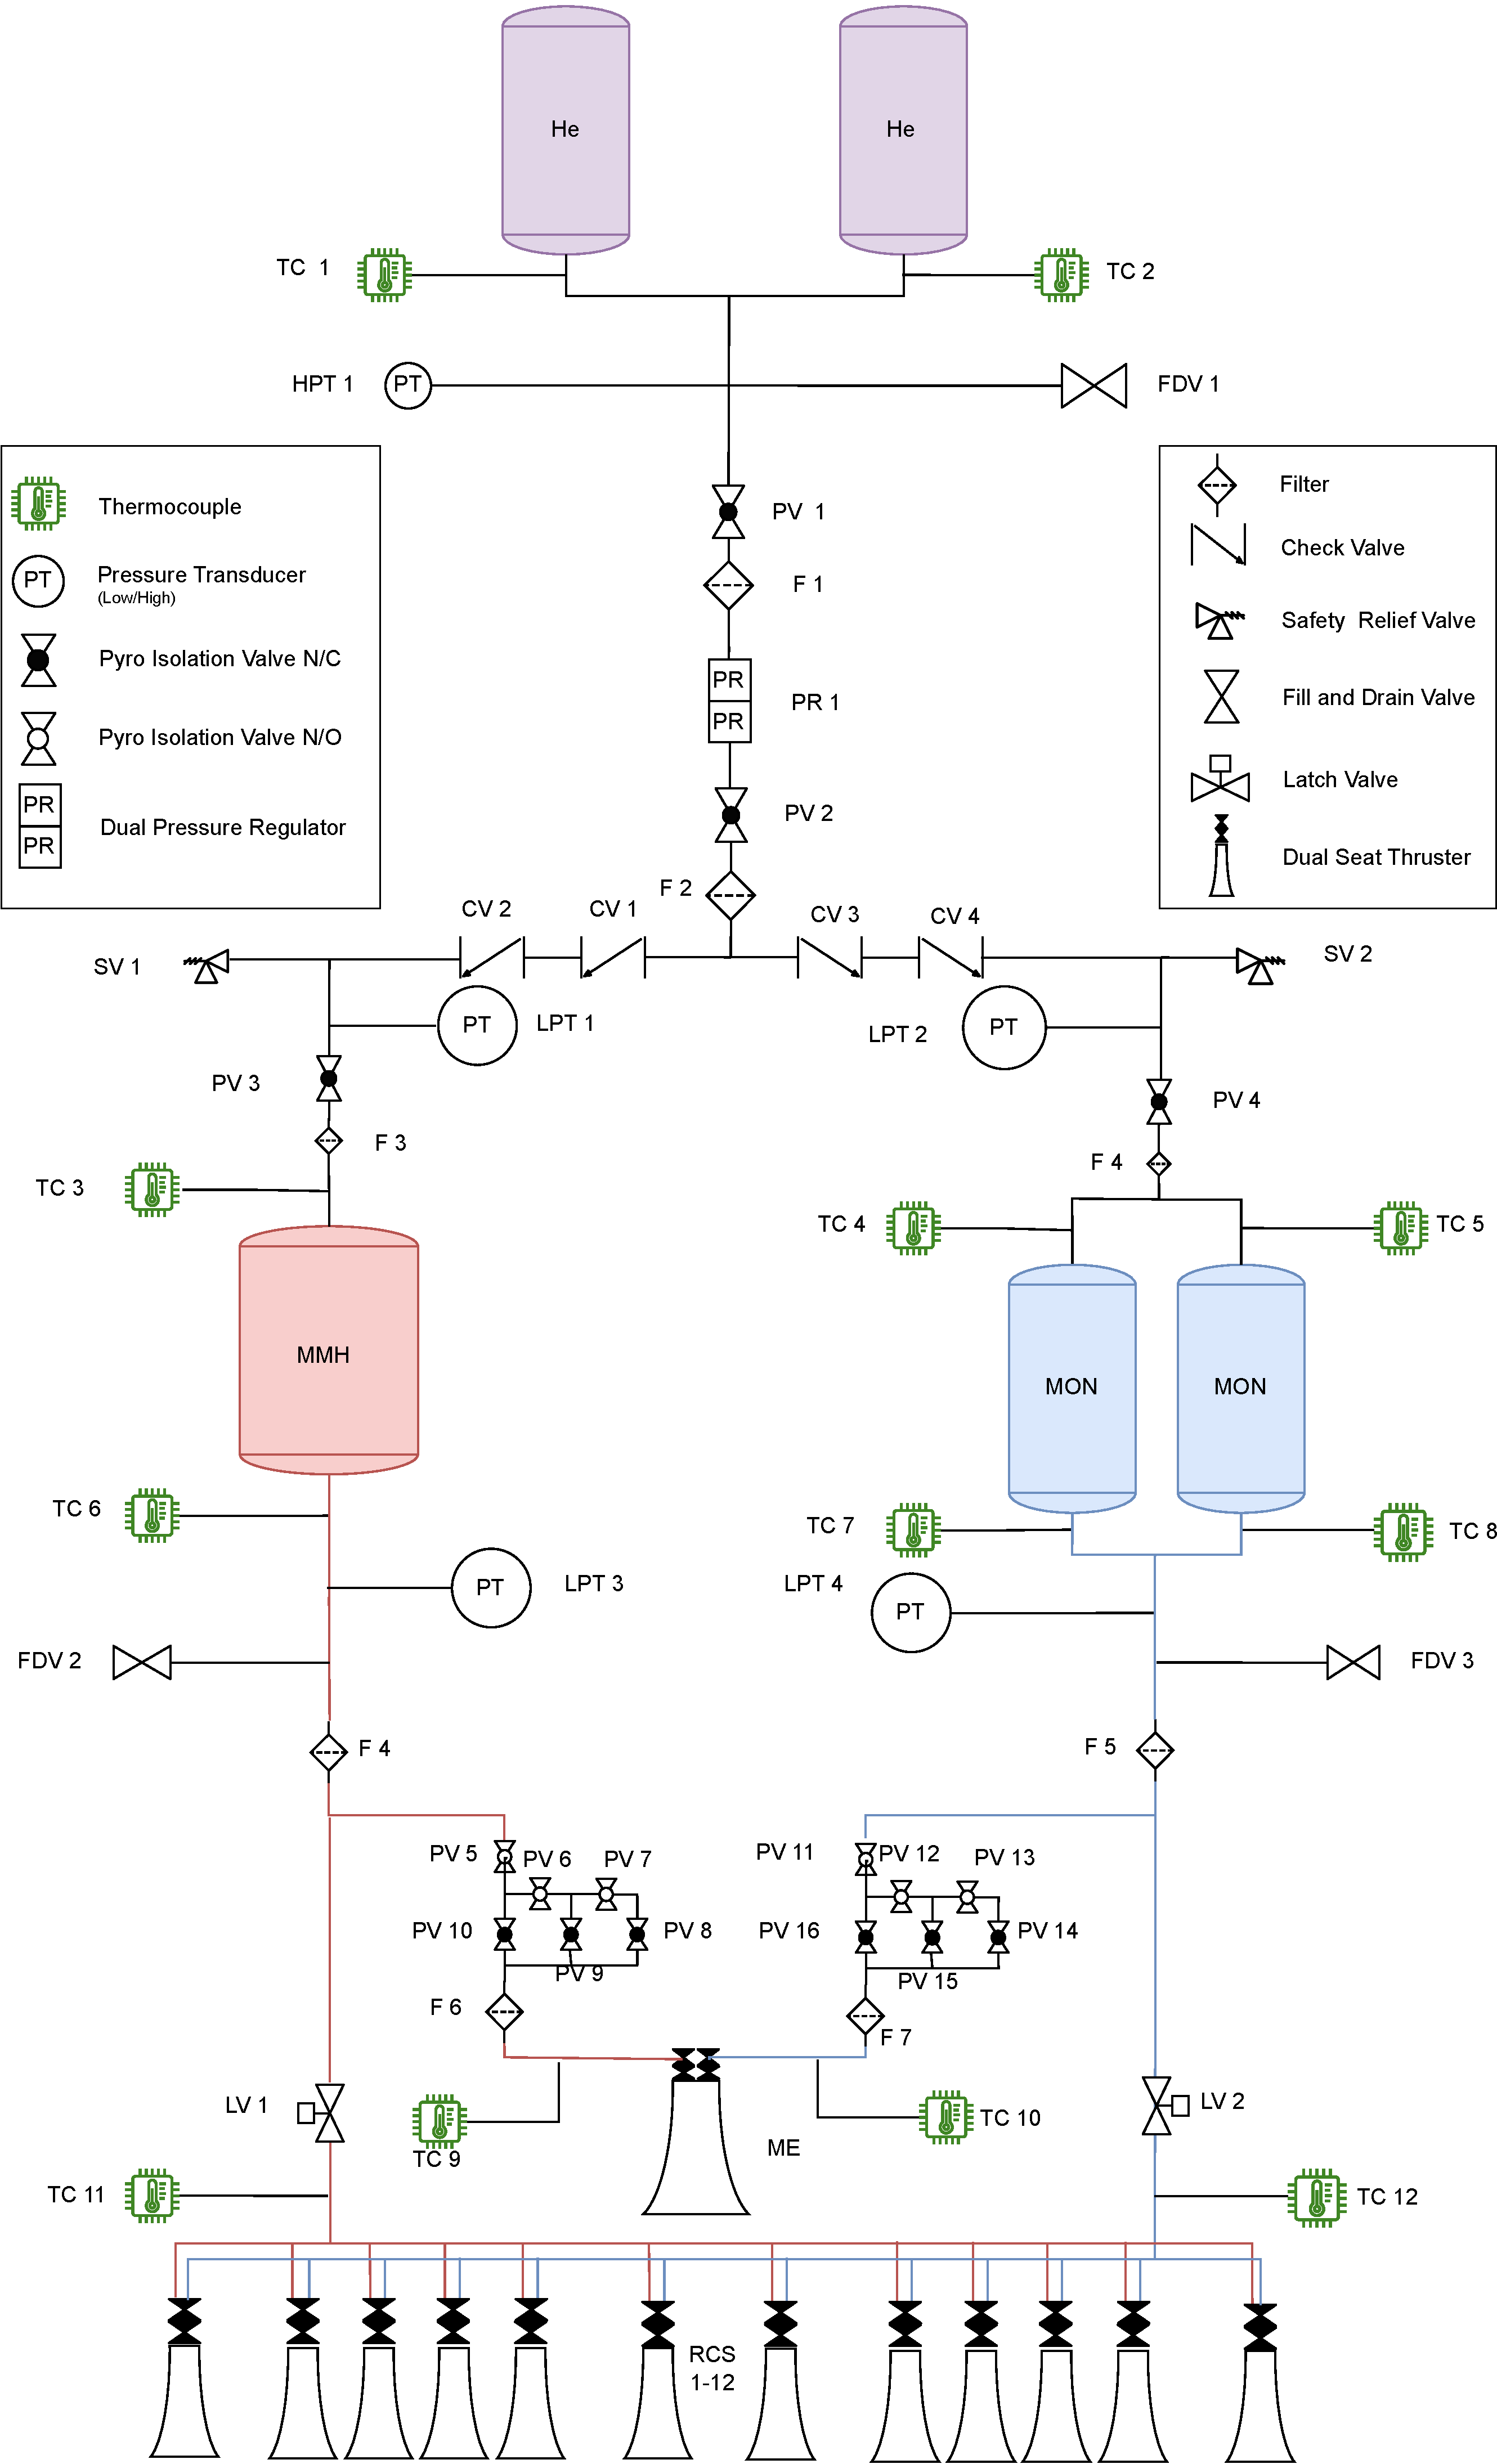
\includegraphics[width=0.79\textwidth]{pdf/Flowchart_Biprop.pdf}
  \caption{Flowchart for Chemical Bipropellant Subsystem}
  \label{fig:flow-biprop}
\end{figure*}


\begin{figure*}[h]
  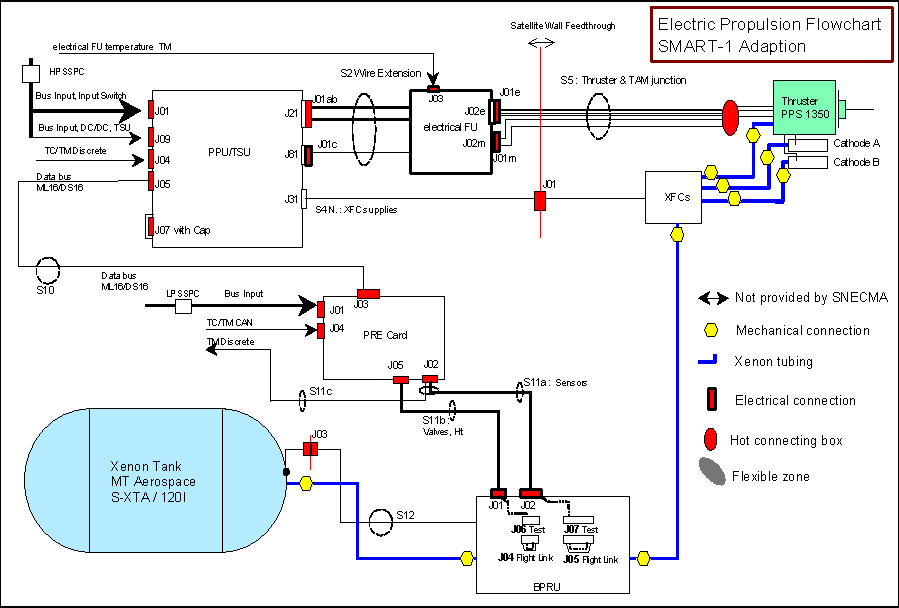
\includegraphics[width=\textwidth]{img/electric_flowchart.pdf}
  \caption{Flowchart for Electrical Propulsion System as Adaption from SMART-1 \cite{Koppel2004}}
  \label{fig:flow-elec}
\end{figure*}

\begin{figure*}[h]
  \centering
  \includegraphics[width=\textwidth]{img/el_hardware.jpg}
  \caption{Electric Propulsion Hardware adapted from SMART-1 \cite{Koppel2004}}
  \label{fig:elec-hardware}
\end{figure*}

\begin{table*}
\caption{Mission Timeline}
\label{tab:mis-timeline}
\resizebox{\linewidth}{!}{%
\begin{tblr}{
  row{1} = {Cornflower},
  row{2} = {Spindle},
  column{1} = {r},
  column{4} = {r},
  column{5} = {r},
  column{6} = {r},
  column{7} = {r},
  column{8} = {r},
  column{9} = {r},
  cell{1}{1} = {c},
  cell{1}{4} = {c},
  cell{1}{5} = {c},
  cell{1}{6} = {c},
  cell{1}{7} = {c},
  cell{1}{8} = {c},
  cell{1}{9} = {c},
  cell{2}{1} = {c},
  cell{2}{4} = {c},
  cell{2}{5} = {c},
  cell{2}{6} = {c},
  cell{2}{7} = {c},
  cell{2}{8} = {c},
  cell{2}{9} = {c},
  hlines,
  vlines,
}
                     & \textbf{} &                        & {[}kg]           & {[}kg]      & {[}kg]       & {[}kg]       & {[}kg]      & {[}kg]              \\
\textbf{Timestamp}   &           & \textbf{Maneuver Name} & \textbf{Drymass} & \textbf{He} & \textbf{MMH} & \textbf{MMO} & \textbf{Xe} & \textbf{Total Mass} \\
31 Oct 2026 12:00:00 &           & Ariane 62 Mounted      & 1226.589         & 3.525       & 283.500      & 467.775      & 166.000     & 2147.390            \\
31 Oct 2026 12:00:37 &           & Ariane 62 Eject        & 1141.589         & 3.525       & 283.500      & 467.775      & 166.000     & 2062.390            \\
03 Nov 2026 12:00:37 & Begin     & C3                     & 1141.589         & 3.525       & 283.500      & 467.775      & 166.000     & 2062.390            \\
03 Nov 2026 12:36:32 & End       & C3                     & 1141.589         & 3.525       & 166.786      & 275.197      & 166.000     & 1753.097            \\
21 Nov 2026 12:36:32 & Begin     & TCM                    & 1141.589         & 3.525       & 166.786      & 275.197      & 166.000     & 1753.097            \\
21 Nov 2026 12:36:38 & End       & TCM                    & 1141.589         & 3.525       & 166.496      & 274.719      & 166.000     & 1752.330            \\
17 Aug 2027 04:48:54 & Begin     & MOI                    & 1141.589         & 3.525       & 166.496      & 274.719      & 166.000     & 1752.330            \\
17 Aug 2027 05:36:32 & End       & MOI                    & 1141.589         & 3.525       & 11.752       & 19.392       & 166.000     & 1342.258            \\
28 Aug 2027 18:17:43 & Begin     & Match INC              & 1141.589         & 3.525       & 11.752       & 19.392       & 166.000     & 1342.258            \\
28 Aug 2027 18:18:25 & End       & Match INC              & 1141.589         & 3.525       & 9.455        & 15.600       & 166.000     & 1336.169            \\
29 Aug 2027 17:36:46 & Begin     & Raise Peri min         & 1141.589         & 3.525       & 9.455        & 15.600       & 166.000     & 1336.169            \\
29 Aug 2027 17:36:59 & End       & Raise Peri min         & 1141.589         & 3.525       & 8.744        & 14.427       & 166.000     & 1334.285            \\
22 Sep 2027 10:44:25 & Begin     & Circularize            & 1141.589         & 3.525       & 8.744        & 14.427       & 166.000     & 1334.285            \\
26 Aug 2029 16:26:15 & End       & Circularize            & 1141.589         & 3.525       & 8.744        & 14.427       & 114.195     & 1282.480            \\
27 Aug 2029 07:10:20 & Begin     & Spiral Down Match      & 1141.589         & 3.525       & 8.744        & 14.427       & 114.195     & 1282.480            \\
01 Jan 2030 14:43:40 & Begin     & Wait Match             & 1141.589         & 3.525       & 8.744        & 14.427       & 58.129      & 1226.414            \\
03 Jan 2030 00:29:49 & End       & Wait Match             & 1141.589         & 3.525       & 8.744        & 14.427       & 58.129      & 1226.414            \\
06 Jan 2030 21:28:19 & End       & Spiral Down Match      & 1141.589         & 3.525       & 8.744        & 14.427       & 56.458      & 1224.744            \\
06 Jan 2030 21:34:01 &           & Arrived - Probe drop   & 1121.589         & 3.525       & 8.744        & 14.427       & 56.458      & 1204.744            \\
                     &           & Orbital Maintenance    & 1121.589         & 3.525       & 8.744        & 14.427       & 49.477      & 1197.762            \\
06 Jan 2032 21:34:01 & Begin     & EOL                    & 1121.589         & 3.525       & 8.744        & 14.427       & 49.477      & 1197.762            \\
20 Apr 2032 12:31:53 & End       & EOL                    & 1121.589         & 3.525       & 8.744        & 14.427       & 3.422       & 1151.708            
\end{tblr}
}
\end{table*}



\begin{table*}
\caption{Electric Thruster Selection}
\label{tab:el-thruster}
\centering
\resizebox{\linewidth}{!}{%
\begin{tblr}{
  row{1} = {Cornflower,c},
  row{2} = {Spindle},
  row{13} = {HintofGreen},
  cell{3}{3} = {r},
  cell{3}{4} = {FairPink,r},
  cell{3}{5} = {r},
  cell{3}{6} = {FairPink,r},
  cell{3}{7} = {r},
  cell{3}{8} = {r},
  cell{3}{9} = {r},
  cell{3}{10} = {r},
  cell{4}{3} = {r},
  cell{4}{4} = {FairPink,r},
  cell{4}{5} = {r},
  cell{4}{6} = {FairPink,r},
  cell{4}{7} = {r},
  cell{4}{8} = {r},
  cell{4}{9} = {r},
  cell{4}{10} = {r},
  cell{5}{3} = {r},
  cell{5}{4} = {FairPink,r},
  cell{5}{5} = {r},
  cell{5}{6} = {FairPink,r},
  cell{5}{7} = {r},
  cell{5}{8} = {r},
  cell{5}{9} = {r},
  cell{5}{10} = {r},
  cell{6}{3} = {r},
  cell{6}{4} = {FairPink,r},
  cell{6}{5} = {r},
  cell{6}{6} = {FairPink,r},
  cell{6}{7} = {r},
  cell{6}{8} = {r},
  cell{6}{9} = {r},
  cell{6}{10} = {r},
  cell{7}{3} = {r},
  cell{7}{4} = {FairPink,r},
  cell{7}{5} = {r},
  cell{7}{6} = {FairPink,r},
  cell{7}{7} = {r},
  cell{7}{8} = {r},
  cell{7}{9} = {r},
  cell{7}{10} = {r},
  cell{8}{3} = {r},
  cell{8}{4} = {r},
  cell{8}{5} = {r},
  cell{8}{6} = {FairPink,r},
  cell{8}{7} = {r},
  cell{8}{8} = {r},
  cell{8}{9} = {r},
  cell{8}{10} = {r},
  cell{9}{3} = {r},
  cell{9}{4} = {r},
  cell{9}{5} = {r},
  cell{9}{6} = {FairPink,r},
  cell{9}{7} = {r},
  cell{9}{8} = {r},
  cell{9}{9} = {r},
  cell{9}{10} = {r},
  cell{10}{3} = {r},
  cell{10}{4} = {r},
  cell{10}{5} = {r},
  cell{10}{6} = {FairPink,r},
  cell{10}{7} = {r},
  cell{10}{8} = {r},
  cell{10}{9} = {r},
  cell{10}{10} = {r},
  cell{11}{3} = {r},
  cell{11}{4} = {r},
  cell{11}{5} = {r},
  cell{11}{6} = {FairPink,r},
  cell{11}{7} = {r},
  cell{11}{8} = {r},
  cell{11}{9} = {r},
  cell{11}{10} = {r},
  cell{12}{3} = {r},
  cell{12}{4} = {r},
  cell{12}{5} = {r},
  cell{12}{6} = {FairPink,r},
  cell{12}{7} = {r},
  cell{12}{8} = {r},
  cell{12}{9} = {r},
  cell{12}{10} = {r},
  cell{13}{3} = {r},
  cell{13}{4} = {r},
  cell{13}{5} = {r},
  cell{13}{6} = {r},
  cell{13}{7} = {r},
  cell{13}{8} = {r},
  cell{13}{9} = {r},
  cell{13}{10} = {r},
  cell{14}{3} = {r},
  cell{14}{4} = {r},
  cell{14}{5} = {r},
  cell{14}{6} = {r},
  cell{14}{7} = {r},
  cell{14}{8} = {r},
  cell{14}{9} = {r},
  cell{14}{10} = {r},
  cell{15}{3} = {r},
  cell{15}{4} = {r},
  cell{15}{5} = {r},
  cell{15}{6} = {r},
  cell{15}{7} = {r},
  cell{15}{8} = {r},
  cell{15}{9} = {r},
  cell{15}{10} = {r},
  cell{16}{3} = {r},
  cell{16}{4} = {r},
  cell{16}{5} = {r},
  cell{16}{6} = {r},
  cell{16}{7} = {r},
  cell{16}{8} = {r},
  cell{16}{9} = {r},
  cell{16}{10} = {r},
  cell{17}{3} = {r},
  cell{17}{4} = {r},
  cell{17}{5} = {r},
  cell{17}{6} = {r},
  cell{17}{7} = {r},
  cell{17}{8} = {r},
  cell{17}{9} = {r},
  cell{17}{10} = {r},
  cell{18}{3} = {r},
  cell{18}{4} = {r},
  cell{18}{5} = {r},
  cell{18}{6} = {r},
  cell{18}{7} = {r},
  cell{18}{8} = {r},
  cell{18}{9} = {r},
  cell{18}{10} = {r},
  cell{19}{3} = {r},
  cell{19}{4} = {FairPink,r},
  cell{19}{5} = {r},
  cell{19}{6} = {FairPink,r},
  cell{19}{7} = {r},
  cell{19}{8} = {r},
  cell{19}{9} = {r},
  cell{19}{10} = {r},
  cell{20}{3} = {r},
  cell{20}{4} = {r},
  cell{20}{5} = {r},
  cell{20}{6} = {FairPink,r},
  cell{20}{7} = {r},
  cell{20}{8} = {r},
  cell{20}{9} = {r},
  cell{20}{10} = {r},
  cell{21}{3} = {r},
  cell{21}{4} = {r},
  cell{21}{5} = {r},
  cell{21}{6} = {FairPink,r},
  cell{21}{7} = {r},
  cell{21}{8} = {r},
  cell{21}{9} = {r},
  cell{21}{10} = {r},
  cell{22}{3} = {r},
  cell{22}{4} = {r},
  cell{22}{5} = {r},
  cell{22}{6} = {FairPink,r},
  cell{22}{7} = {r},
  cell{22}{8} = {r},
  cell{22}{9} = {r},
  cell{22}{10} = {r},
  cell{23}{3} = {r},
  cell{23}{4} = {r},
  cell{23}{5} = {r},
  cell{23}{6} = {FairPink,r},
  cell{23}{7} = {r},
  cell{23}{8} = {r},
  cell{23}{9} = {r},
  cell{23}{10} = {r},
  cell{24}{3} = {r},
  cell{24}{4} = {r},
  cell{24}{5} = {r},
  cell{24}{6} = {r},
  cell{24}{7} = {r},
  cell{24}{8} = {r},
  cell{24}{9} = {r},
  cell{24}{10} = {r},
  cell{25}{3} = {r},
  cell{25}{4} = {r},
  cell{25}{5} = {r},
  cell{25}{6} = {r},
  cell{25}{7} = {r},
  cell{25}{8} = {r},
  cell{25}{9} = {r},
  cell{25}{10} = {r},
  cell{26}{3} = {r},
  cell{26}{4} = {r},
  cell{26}{5} = {r},
  cell{26}{6} = {r},
  cell{26}{7} = {r},
  cell{26}{8} = {r},
  cell{26}{9} = {r},
  cell{26}{10} = {r},
  cell{27}{3} = {r},
  cell{27}{4} = {r},
  cell{27}{5} = {r},
  cell{27}{6} = {r},
  cell{27}{7} = {r},
  cell{27}{8} = {r},
  cell{27}{9} = {r},
  cell{27}{10} = {r},
  cell{28}{3} = {r},
  cell{28}{4} = {r},
  cell{28}{5} = {r},
  cell{28}{6} = {r},
  cell{28}{7} = {r},
  cell{28}{8} = {r},
  cell{28}{9} = {r},
  cell{28}{10} = {r},
  hlines,
  vlines,
}
Manufacturer   & Name       & Power & Thrust & Isp   & Burntime   & Fuel Mass & Solar Mass & Sum Mass & Launch Mass \\
               &            & {[}W] & {[}mN] & {[}s] & {[}years]  & {[}kg]    & {[}kg]     & {[}kg]   & {[}kg]      \\
Morpheus Space & NanoFEEP   & 0.2   & 0.001  & 3000  & 83443.5960 & 89.45     & 0.04       & 89.64    &             \\
               &            & 3     & 0.02   & 8500  & 4314.1692  & 32.64     & 0.53       & 33.33    &             \\
Morpheus Space & MultiFEEP  & 0.4   & 0.001  & 7000  & 85944.8386 & 39.48     & 0.07       & 39.85    &             \\
               &            & 1090  & 12.5   & 7000  & 6.8756     & 39.48     & 191.90     & 258.98   &             \\
Rafael         & R-200      & 140   & 4      & 800   & 18.1724    & 292.19    & 24.65      & 316.84   &             \\
               &            & 350   & 14     & 1300  & 5.5770     & 193.14    & 61.62      & 254.76   &             \\
Rafael         & R-800      & 500   & 23     & 1300  & 3.3947     & 193.14    & 88.03      & 281.16   &             \\
               &            & 1000  & 53     & 1550  & 1.5011     & 165.05    & 176.05     & 341.11   &             \\
Safran         & PPS X00    & 200   & 15     & 1300  & 5.2052     & 193.14    & 35.21      & 228.35   &             \\
               &            & 1000  & 75     & 1650  & 1.0671     & 155.97    & 176.05     & 342.03   &             \\
Safran         & PPS 1350-G & 1500  & 90     & 1800  & 0.8961     & 144.08    & 264.08     & 437.16   & 1993.5841   \\
               &            & 2500  & 140    & 1800  & 0.5761     & 144.08    & 440.13     & 613.21   & 2487.5044   \\
Safran         & PPS 1350-E & 2500  & 100    & 1600  & 0.7980     & 160.39    & 440.13     & 600.51   & 2547.0515   \\
               &            & 5000  & 300    & 1900  & 0.2700     & 137.11    & 880.26     & 1017.36  & 3685.1358   \\
Safran         & PPS 5000   & 2500  & 150    & 1730  & 0.5358     & 149.40    & 440.13     & 615.53   & 2529.7035   \\
               &            & 5000  & 300    & 2000  & 0.2711     & 130.78    & 880.26     & 1043.03  & 3683.8819   \\
ArianeGroup    & RIT uX     & 50    & 0.5    & 3000  & 166.8872   & 89.45     & 8.80       & 98.25    &             \\
ArianeGroup    & RIT 10 EVO & 145   & 5      & 1900  & 16.2017    & 137.11    & 25.53      & 162.64   &             \\
               &            & 435   & 15     & 3000  & 5.5629     & 89.45     & 76.58      & 166.03   &             \\
               &            & 760   & 25     & 3200  & 3.3485     & 84.13     & 133.80     & 217.92   &             \\
ArianeGroup    & RIT 2X     & 2000  & 70     & 3400  & 1.1993     & 79.40     & 352.10     & 431.50   & 2053.9215   \\
               &            & 2500  & 88     & 3500  & 0.9552     & 77.23     & 440.13     & 517.36   & 2273.0878   \\
               &            & 4000  & 151    & 3300  & 0.5552     & 81.70     & 704.21     & 785.90   & 2964.5545   \\
               &            & 4500  & 171    & 3500  & 0.4916     & 77.23     & 792.23     & 869.46   & 3172.3386   \\
               &            & 4800  & 198    & 2450  & 0.4166     & 108.27    & 845.05     & 953.32   & 3446.0344   \\
               &            & 5300  & 215    & 2750  & 0.3863     & 97.12     & 933.07     & 1030.19  & 3625.6223   
\end{tblr}
}
\end{table*}


\begin{table*}[]
\caption{Tank Database}
\label{tab:tank-tit}
\resizebox{\linewidth}{!}{%
\begin{tabular}{|ccccc|}
\hline
\multicolumn{5}{|c|}{\cellcolor[HTML]{8DB4E1}\textbf{Titanium Tanks (Monoprop / Biprop)}}                                                                                                                                                                                                                                   \\ \hline
\multicolumn{1}{|c|}{\textbf{Volume {[}l{]}}} & \multicolumn{1}{c|}{\textbf{Ideal mass {[}kg{]}}} & \multicolumn{1}{c|}{\textbf{Real mass {[}kg{]}}} & \multicolumn{1}{c|}{\textbf{Margin-factor}}       & \textbf{Tank Source}                                                                                             \\ \hline
\multicolumn{1}{|c|}{}                        & \multicolumn{1}{c|}{}                             & \multicolumn{1}{c|}{}                            & \multicolumn{1}{c|}{}                             &                                                                                                                  \\ \hline
\multicolumn{1}{|c|}{304}                     & \multicolumn{1}{c|}{8.9643}                       & \multicolumn{1}{c|}{17.5}                        & \multicolumn{1}{c|}{1.95}                         & {\color[HTML]{0000FF} https://www.space-propulsion.com/spacecraft-propulsion/bipropellant-tanks/index.html\#198} \\ \hline
\multicolumn{1}{|c|}{218}                     & \multicolumn{1}{c|}{6.4284}                       & \multicolumn{1}{c|}{11}                          & \multicolumn{1}{c|}{1.71}                         & https://www.space-propulsion.com/spacecraft-propulsion/bipropellant-tanks/index.html\#199                        \\ \hline
\multicolumn{1}{|c|}{235}                     & \multicolumn{1}{c|}{6.9297}                       & \multicolumn{1}{c|}{16}                          & \multicolumn{1}{c|}{2.31}                         & https://www.space-propulsion.com/spacecraft-propulsion/bipropellant-tanks/index.html\#200                        \\ \hline
\multicolumn{1}{|c|}{282}                     & \multicolumn{1}{c|}{8.3156}                       & \multicolumn{1}{c|}{21}                          & \multicolumn{1}{c|}{2.53}                         & https://www.space-propulsion.com/spacecraft-propulsion/bipropellant-tanks/index.html\#201                        \\ \hline
\multicolumn{1}{|c|}{331}                     & \multicolumn{1}{c|}{8.6514}                       & \multicolumn{1}{c|}{22.7}                        & \multicolumn{1}{c|}{2.62}                         & https://www.space-propulsion.com/spacecraft-propulsion/bipropellant-tanks/index.html\#202                        \\ \hline
\multicolumn{1}{|c|}{700}                     & \multicolumn{1}{c|}{18.2959}                      & \multicolumn{1}{c|}{36}                          & \multicolumn{1}{c|}{1.97}                         & https://www.space-propulsion.com/spacecraft-propulsion/bipropellant-tanks/index.html\#203                        \\ \hline
\multicolumn{1}{|c|}{1108}                    & \multicolumn{1}{c|}{28.9598}                      & \multicolumn{1}{c|}{49}                          & \multicolumn{1}{c|}{1.69}                         & https://www.space-propulsion.com/spacecraft-propulsion/bipropellant-tanks/index.html\#204                        \\ \hline
\multicolumn{1}{|c|}{769}                     & \multicolumn{1}{c|}{18.0379}                      & \multicolumn{1}{c|}{31.7}                        & \multicolumn{1}{c|}{1.76}                         & https://www.space-propulsion.com/spacecraft-propulsion/bipropellant-tanks/index.html\#205                        \\ \hline
\multicolumn{1}{|c|}{1207}                    & \multicolumn{1}{c|}{31.5474}                      & \multicolumn{1}{c|}{52.5}                        & \multicolumn{1}{c|}{1.66}                         & https://www.space-propulsion.com/spacecraft-propulsion/bipropellant-tanks/index.html\#206                        \\ \hline
\multicolumn{1}{|c|}{1309}                    & \multicolumn{1}{c|}{34.2134}                      & \multicolumn{1}{c|}{57}                          & \multicolumn{1}{c|}{1.67}                         & https://www.space-propulsion.com/spacecraft-propulsion/bipropellant-tanks/index.html\#207                        \\ \hline
\multicolumn{1}{|c|}{1450}                    & \multicolumn{1}{c|}{37.8987}                      & \multicolumn{1}{c|}{61}                          & \multicolumn{1}{c|}{1.61}                         & https://www.space-propulsion.com/spacecraft-propulsion/bipropellant-tanks/index.html\#208                        \\ \hline
\multicolumn{1}{|c|}{165}                     & \multicolumn{1}{c|}{4.4232}                       & \multicolumn{1}{c|}{10.8}                        & \multicolumn{1}{c|}{2.44}                         & https://www.mt-aerospace.de/files/mta/tankkatalog/MT-Tankkatalog.pdf                                             \\ \hline
\multicolumn{1}{|c|}{}                        & \multicolumn{1}{c|}{}                             & \multicolumn{1}{c|}{}                            & \multicolumn{1}{c|}{}                             &                                                                                                                  \\ \hline
\multicolumn{1}{|c|}{}                        & \multicolumn{1}{c|}{}                             & \multicolumn{1}{c|}{}                            & \multicolumn{1}{c|}{{\color[HTML]{FF6D01} 1.993}} &                                                                                                                  \\ \hline
\multicolumn{5}{|c|}{\cellcolor[HTML]{8DB4E1}\textbf{CFRP-Titanium Tanks   (Xenon)}}                                                                                                                                                                                                                                        \\ \hline
\multicolumn{1}{|c|}{\textbf{Volume {[}l{]}}} & \multicolumn{1}{c|}{\textbf{Ideal mass {[}kg{]}}} & \multicolumn{1}{c|}{\textbf{Real mass {[}kg{]}}} & \multicolumn{1}{c|}{\textbf{Margin-factor}}       & \textbf{Tank Source}                                                                                             \\ \hline
\multicolumn{1}{|c|}{}                        & \multicolumn{1}{c|}{}                             & \multicolumn{1}{c|}{}                            & \multicolumn{1}{c|}{}                             &                                                                                                                  \\ \hline
\multicolumn{1}{|c|}{60}                      & \multicolumn{1}{c|}{4.1329}                       & \multicolumn{1}{c|}{11.7}                        & \multicolumn{1}{c|}{2.83}                         & https://www.mt-aerospace.de/files/mta/tankkatalog/MT-Tankkatalog.pdf                                             \\ \hline
\multicolumn{1}{|c|}{40}                      & \multicolumn{1}{c|}{2.7553}                       & \multicolumn{1}{c|}{6.3}                         & \multicolumn{1}{c|}{2.29}                         & https://www.mt-aerospace.de/files/mta/tankkatalog/MT-Tankkatalog.pdf                                             \\ \hline
\multicolumn{1}{|c|}{120}                     & \multicolumn{1}{c|}{8.2658}                       & \multicolumn{1}{c|}{14.8}                        & \multicolumn{1}{c|}{1.79}                         & https://www.mt-aerospace.de/files/mta/tankkatalog/MT-Tankkatalog.pdf                                             \\ \hline
\multicolumn{1}{|c|}{600}                     & \multicolumn{1}{c|}{41.3288}                      & \multicolumn{1}{c|}{68}                          & \multicolumn{1}{c|}{1.65}                         & https://www.mt-aerospace.de/files/mta/tankkatalog/MT-Tankkatalog.pdf                                             \\ \hline
\multicolumn{1}{|c|}{900}                     & \multicolumn{1}{c|}{61.9932}                      & \multicolumn{1}{c|}{85}                          & \multicolumn{1}{c|}{1.37}                         & https://www.mt-aerospace.de/files/mta/tankkatalog/MT-Tankkatalog.pdf                                             \\ \hline
\multicolumn{1}{|c|}{}                        & \multicolumn{1}{c|}{}                             & \multicolumn{1}{c|}{}                            & \multicolumn{1}{c|}{}                             &                                                                                                                  \\ \hline
\multicolumn{1}{|c|}{}                        & \multicolumn{1}{c|}{}                             & \multicolumn{1}{c|}{}                            & \multicolumn{1}{c|}{{\color[HTML]{4285F4} 1.985}} &                                                                                                                  \\ \hline
\multicolumn{5}{|c|}{\cellcolor[HTML]{8DB4E1}\textbf{CFRP-Titanium Tanks   (Helium, Nitrogen)}}                                                                                                                                                                                                                             \\ \hline
\multicolumn{1}{|c|}{\textbf{Volume {[}l{]}}} & \multicolumn{1}{c|}{\textbf{Ideal mass {[}kg{]}}} & \multicolumn{1}{c|}{\textbf{Real mass {[}kg{]}}} & \multicolumn{1}{c|}{\textbf{Margin-factor}}       & \textbf{Tank Source}                                                                                             \\ \hline
\multicolumn{1}{|c|}{}                        & \multicolumn{1}{c|}{}                             & \multicolumn{1}{c|}{}                            & \multicolumn{1}{c|}{}                             &                                                                                                                  \\ \hline
\multicolumn{1}{|c|}{40}                      & \multicolumn{1}{c|}{4.5675}                       & \multicolumn{1}{c|}{8.5}                         & \multicolumn{1}{c|}{1.86}                         & https://www.mt-aerospace.de/files/mta/tankkatalog/MT-Tankkatalog.pdf                                             \\ \hline
\multicolumn{1}{|c|}{75}                      & \multicolumn{1}{c|}{8.5641}                       & \multicolumn{1}{c|}{14.4}                        & \multicolumn{1}{c|}{1.68}                         & https://www.mt-aerospace.de/files/mta/tankkatalog/MT-Tankkatalog.pdf                                             \\ \hline
\multicolumn{1}{|c|}{120}                     & \multicolumn{1}{c|}{13.7026}                      & \multicolumn{1}{c|}{23.5}                        & \multicolumn{1}{c|}{1.72}                         & https://www.mt-aerospace.de/files/mta/tankkatalog/MT-Tankkatalog.pdf                                             \\ \hline
\multicolumn{1}{|c|}{}                        & \multicolumn{1}{c|}{}                             & \multicolumn{1}{c|}{}                            & \multicolumn{1}{c|}{}                             &                                                                                                                  \\ \hline
\multicolumn{1}{|c|}{}                        & \multicolumn{1}{c|}{}                             & \multicolumn{1}{c|}{}                            & \multicolumn{1}{c|}{{\color[HTML]{34A853} 1.752}} &                                                                                                                  \\ \hline
\end{tabular}}
\end{table*}

\begin{sidewaysfigure*}[h]
    \centering
    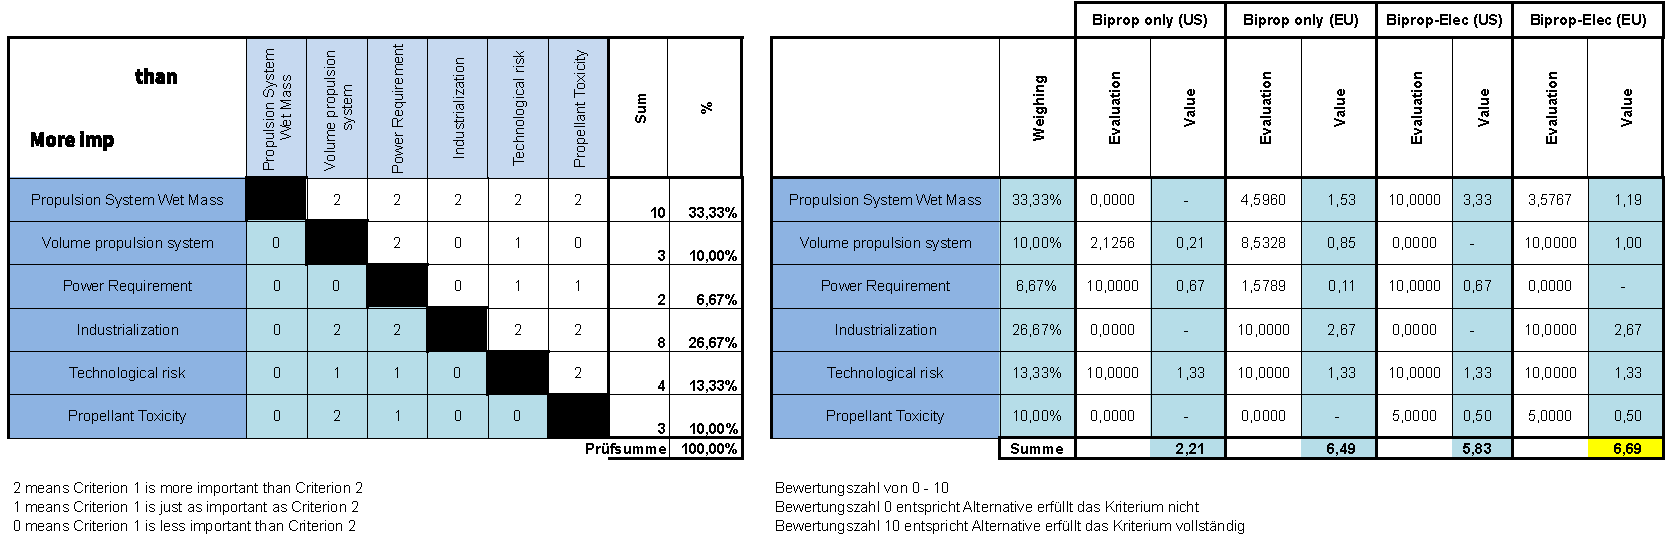
\includegraphics[width=\textwidth]{pdf/PaarwiseAnalysis.pdf} 
    \caption{Criteria Definition}
    \label{fig:par-an}
\end{sidewaysfigure*}


\begin{sidewaysfigure*}[h]
    \centering
    \includegraphics[width=\textwidth]{img/ProjectPlan.png}
    \caption{MomenTUM Project Plan}
    \label{fig:pr-plan}
\end{sidewaysfigure*}

\begin{sidewaysfigure*}[h]
    \centering
    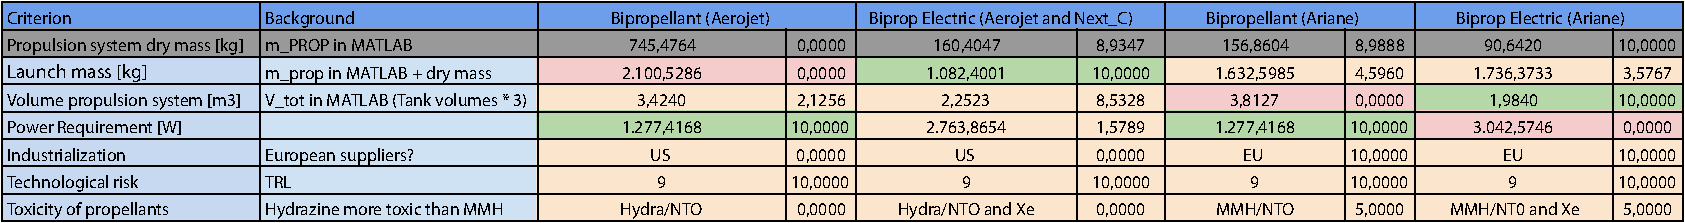
\includegraphics[width=\textwidth]{pdf/CriteriaDefinition.pdf} 
    \caption{Criteria Definition}
    \label{fig:cr-def}
\end{sidewaysfigure*}


\begin{figure*}[h] 
  \centering
  \includegraphics[width=0.6\textwidth]{img/pointmass_XY.jpg}
  \caption{Point-Mass Arrangement in the XY-plane}
  \label{fig:araxy}
\end{figure*}

\begin{figure*}[h]
  \centering
  \includegraphics[width=0.7\textwidth]{img/pointmass_YZ.jpg}
  \caption{Section of the Point-Mass Arrangement in the YZ-plane}
  \label{fig:arayz}
\end{figure*}


\end{document}

